% Options for packages loaded elsewhere
\PassOptionsToPackage{unicode}{hyperref}
\PassOptionsToPackage{hyphens}{url}
%
\documentclass[
]{book}
\title{Coding in R}
\usepackage{etoolbox}
\makeatletter
\providecommand{\subtitle}[1]{% add subtitle to \maketitle
  \apptocmd{\@title}{\par {\large #1 \par}}{}{}
}
\makeatother
\subtitle{An introduction to practical programming in R}
\author{Gaston Sanchez}
\date{2022-02-11}

\usepackage{amsmath,amssymb}
\usepackage{lmodern}
\usepackage{iftex}
\ifPDFTeX
  \usepackage[T1]{fontenc}
  \usepackage[utf8]{inputenc}
  \usepackage{textcomp} % provide euro and other symbols
\else % if luatex or xetex
  \usepackage{unicode-math}
  \defaultfontfeatures{Scale=MatchLowercase}
  \defaultfontfeatures[\rmfamily]{Ligatures=TeX,Scale=1}
\fi
% Use upquote if available, for straight quotes in verbatim environments
\IfFileExists{upquote.sty}{\usepackage{upquote}}{}
\IfFileExists{microtype.sty}{% use microtype if available
  \usepackage[]{microtype}
  \UseMicrotypeSet[protrusion]{basicmath} % disable protrusion for tt fonts
}{}
\makeatletter
\@ifundefined{KOMAClassName}{% if non-KOMA class
  \IfFileExists{parskip.sty}{%
    \usepackage{parskip}
  }{% else
    \setlength{\parindent}{0pt}
    \setlength{\parskip}{6pt plus 2pt minus 1pt}}
}{% if KOMA class
  \KOMAoptions{parskip=half}}
\makeatother
\usepackage{xcolor}
\IfFileExists{xurl.sty}{\usepackage{xurl}}{} % add URL line breaks if available
\IfFileExists{bookmark.sty}{\usepackage{bookmark}}{\usepackage{hyperref}}
\hypersetup{
  pdftitle={Coding in R},
  pdfauthor={Gaston Sanchez},
  hidelinks,
  pdfcreator={LaTeX via pandoc}}
\urlstyle{same} % disable monospaced font for URLs
\usepackage{color}
\usepackage{fancyvrb}
\newcommand{\VerbBar}{|}
\newcommand{\VERB}{\Verb[commandchars=\\\{\}]}
\DefineVerbatimEnvironment{Highlighting}{Verbatim}{commandchars=\\\{\}}
% Add ',fontsize=\small' for more characters per line
\usepackage{framed}
\definecolor{shadecolor}{RGB}{248,248,248}
\newenvironment{Shaded}{\begin{snugshade}}{\end{snugshade}}
\newcommand{\AlertTok}[1]{\textcolor[rgb]{0.94,0.16,0.16}{#1}}
\newcommand{\AnnotationTok}[1]{\textcolor[rgb]{0.56,0.35,0.01}{\textbf{\textit{#1}}}}
\newcommand{\AttributeTok}[1]{\textcolor[rgb]{0.77,0.63,0.00}{#1}}
\newcommand{\BaseNTok}[1]{\textcolor[rgb]{0.00,0.00,0.81}{#1}}
\newcommand{\BuiltInTok}[1]{#1}
\newcommand{\CharTok}[1]{\textcolor[rgb]{0.31,0.60,0.02}{#1}}
\newcommand{\CommentTok}[1]{\textcolor[rgb]{0.56,0.35,0.01}{\textit{#1}}}
\newcommand{\CommentVarTok}[1]{\textcolor[rgb]{0.56,0.35,0.01}{\textbf{\textit{#1}}}}
\newcommand{\ConstantTok}[1]{\textcolor[rgb]{0.00,0.00,0.00}{#1}}
\newcommand{\ControlFlowTok}[1]{\textcolor[rgb]{0.13,0.29,0.53}{\textbf{#1}}}
\newcommand{\DataTypeTok}[1]{\textcolor[rgb]{0.13,0.29,0.53}{#1}}
\newcommand{\DecValTok}[1]{\textcolor[rgb]{0.00,0.00,0.81}{#1}}
\newcommand{\DocumentationTok}[1]{\textcolor[rgb]{0.56,0.35,0.01}{\textbf{\textit{#1}}}}
\newcommand{\ErrorTok}[1]{\textcolor[rgb]{0.64,0.00,0.00}{\textbf{#1}}}
\newcommand{\ExtensionTok}[1]{#1}
\newcommand{\FloatTok}[1]{\textcolor[rgb]{0.00,0.00,0.81}{#1}}
\newcommand{\FunctionTok}[1]{\textcolor[rgb]{0.00,0.00,0.00}{#1}}
\newcommand{\ImportTok}[1]{#1}
\newcommand{\InformationTok}[1]{\textcolor[rgb]{0.56,0.35,0.01}{\textbf{\textit{#1}}}}
\newcommand{\KeywordTok}[1]{\textcolor[rgb]{0.13,0.29,0.53}{\textbf{#1}}}
\newcommand{\NormalTok}[1]{#1}
\newcommand{\OperatorTok}[1]{\textcolor[rgb]{0.81,0.36,0.00}{\textbf{#1}}}
\newcommand{\OtherTok}[1]{\textcolor[rgb]{0.56,0.35,0.01}{#1}}
\newcommand{\PreprocessorTok}[1]{\textcolor[rgb]{0.56,0.35,0.01}{\textit{#1}}}
\newcommand{\RegionMarkerTok}[1]{#1}
\newcommand{\SpecialCharTok}[1]{\textcolor[rgb]{0.00,0.00,0.00}{#1}}
\newcommand{\SpecialStringTok}[1]{\textcolor[rgb]{0.31,0.60,0.02}{#1}}
\newcommand{\StringTok}[1]{\textcolor[rgb]{0.31,0.60,0.02}{#1}}
\newcommand{\VariableTok}[1]{\textcolor[rgb]{0.00,0.00,0.00}{#1}}
\newcommand{\VerbatimStringTok}[1]{\textcolor[rgb]{0.31,0.60,0.02}{#1}}
\newcommand{\WarningTok}[1]{\textcolor[rgb]{0.56,0.35,0.01}{\textbf{\textit{#1}}}}
\usepackage{longtable,booktabs,array}
\usepackage{calc} % for calculating minipage widths
% Correct order of tables after \paragraph or \subparagraph
\usepackage{etoolbox}
\makeatletter
\patchcmd\longtable{\par}{\if@noskipsec\mbox{}\fi\par}{}{}
\makeatother
% Allow footnotes in longtable head/foot
\IfFileExists{footnotehyper.sty}{\usepackage{footnotehyper}}{\usepackage{footnote}}
\makesavenoteenv{longtable}
\usepackage{graphicx}
\makeatletter
\def\maxwidth{\ifdim\Gin@nat@width>\linewidth\linewidth\else\Gin@nat@width\fi}
\def\maxheight{\ifdim\Gin@nat@height>\textheight\textheight\else\Gin@nat@height\fi}
\makeatother
% Scale images if necessary, so that they will not overflow the page
% margins by default, and it is still possible to overwrite the defaults
% using explicit options in \includegraphics[width, height, ...]{}
\setkeys{Gin}{width=\maxwidth,height=\maxheight,keepaspectratio}
% Set default figure placement to htbp
\makeatletter
\def\fps@figure{htbp}
\makeatother
\setlength{\emergencystretch}{3em} % prevent overfull lines
\providecommand{\tightlist}{%
  \setlength{\itemsep}{0pt}\setlength{\parskip}{0pt}}
\setcounter{secnumdepth}{5}
\usepackage{booktabs}
\ifLuaTeX
  \usepackage{selnolig}  % disable illegal ligatures
\fi
\usepackage[]{natbib}
\bibliographystyle{apalike}

\begin{document}
\maketitle

{
\setcounter{tocdepth}{1}
\tableofcontents
}
\hypertarget{welcome}{%
\chapter*{Welcome}\label{welcome}}
\addcontentsline{toc}{chapter}{Welcome}

This book is a work in progress for an introductory textbook on programming in R.

In a nutshell, we discuss the basics of R, covering properties of data objects,
such as vectors, factors, matrices, data frames, and lists. We also cover
main principles for data manipulation, reshaping, tidying, etc. Likewise, we
discuss fundamental notions of programming (e.g.~functions, conditionals,
iterations). And last but not least we describe how to make basic (and not so
basic) graphics.

\hypertarget{yet-another-r-book}{%
\section*{Yet Another R Book}\label{yet-another-r-book}}
\addcontentsline{toc}{section}{Yet Another R Book}

Why writing another book about programming in R? Quick answer: ``Why not?''
The truth is that for many years I refrained myself from writing a book like
the one you are reading now. I used to tell myself something along the lines
of: ``The world does not need another introductory book about R.'' And I still
somewhat agree with this. Okay, maybe the world does not need another book
like this \ldots{} but I do.

After using R---almost on a daily basis---for more than 16 years, and
having taught STAT 133 ``Concepts in Computing with Data'', for the past 6 years,
I've accumulated a large body of notes, slides, scripts, exercises and that
sort of things, that deserve a place such as this a textbook. In addition, and
more important, it fits my needs for teaching courses such as STAT 133, STAT 33A,
STAT 33B, STAT 243, and similar courses on programming, data analysis, data
science, and related activities \ldots{} with R.

As you will see, the book has an overarching theme based on financial math
formulas and personal finance applications. The main reason for this decision
is to provide a unifying theme under which most topics can be tidely presented,
instead of offering a number of examples in a vacuum.

I hope you enjoy reading the book, learn something (hopefully a lot) about
coding in R, and also a bit of financial math. Enough chit-chat.
Let's get started.

\hypertarget{part-getting-started-with-r-and-rstudio}{%
\part{Getting Started with R and RStudio}\label{part-getting-started-with-r-and-rstudio}}

\hypertarget{install}{%
\chapter{Installing R and RStudio}\label{install}}

To learn how to program in R, you obviously need to have access to it. This
chapter guides you through the installation process so that you can have both R
and RStudio up and running in your computer.

If you already have R and RStudio installed in your machine, you can safely
skip this chapter.

\hypertarget{interacting-with-r}{%
\section{Interacting with R}\label{interacting-with-r}}

Before I show you how to install R and the integrated development environment
RStudio, let me tell you first about the different ways in which users can
work with R.

Overall, you can work with R in two major ways:

\begin{enumerate}
\def\labelenumi{\arabic{enumi})}
\item
  Interactive Mode, and
\item
  Non-interactive Mode
\end{enumerate}

\textbf{Interactive Mode.} Most R users work with R in an interactive way, and this
is certainly the way I personally interact with R in my daily coding activities.
Interactive means that you launch R (i.e.~you open a session), having direct
access to its console. This is where you type in commands, and then R does its
magic reading the commands, parsing them, evaluating them,
and---typically---printing an output back into the console, waiting for you to
type in the next command(s).

\textbf{Non-interactive Mode.} In contrast to interactive mode, working with R in non-interactive way involves writing all the commands in a text file (for
example in an \texttt{R} script file), and then asking your computer---via the
command line interface---to pass this file to R so that it runs the
commands without you launching R or having direct access to its console.

Think of interactive way as having a direct conversation with R, establishing
a dialogue in which you type in a command, R interprets it, gives you an
answer, and then you type more commands, continuing the dialogue. In constrast,
non-interactive is like writing a letter (or an email) to R. Here you don't
have that synchronous conversation, instead R will see the script file, try to
execute all the commands ``behind the scenes'', and it will disappear when it
finishes the computations. You may get some output back, but R is gone in the
sense that there is no open session waiting for you to execute the next
instructions.

Most of what I discuss in this book is applicable to writing code in R
regardless of how you decide to interact with R. However, to learn R and to
follow the examples of the book it is definitely much better to do it in an
interactive way using: a) R's built-in graphical user interface (R's GUI),
b) an integrated development environment (IDE) such as RStudio, or
c) R from a command line interface (CLI) commonly referred to as a \emph{terminal}.

\begin{figure}

{\centering 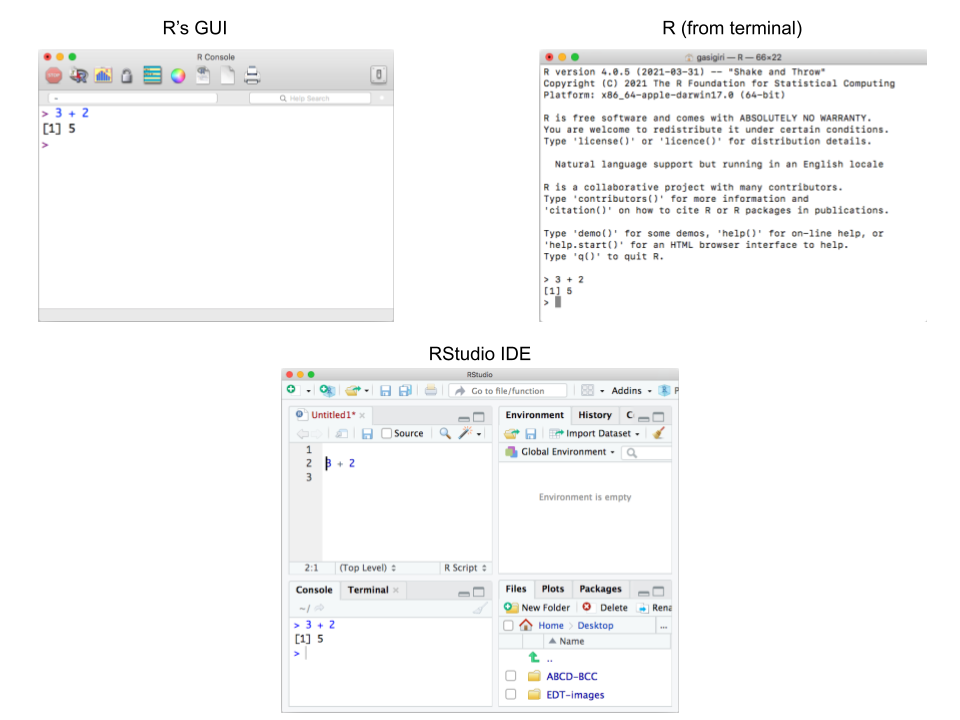
\includegraphics[width=0.9\linewidth]{images/install/r-interactive-ways} 

}

\caption{Interacting with R in various ways: R's GUI, RStudio, and R from a command-line terminal}\label{fig:unnamed-chunk-3}
\end{figure}

While you can interact with R using its built-in graphical user interface (GUI)
or launching R from the terminal (command line interface), nowadays I highly
recommend that you interact with it using an
\emph{Integrated Development Environment} (IDE) such as
\href{https://www.rstudio.com/}{\textbf{RStudio}}. Simply put,
programs like RStudio provide a nice working space that make your life easier
while writing code, creating all sorts of reports, documents, and slides,
running analysis, making graphs, generating outputs, creating web apps, etc.

\begin{figure}

{\centering 
\includegraphics[width=0.3\linewidth]{images/rstudio/r-rstudio-logos} 

}

\caption{Main computational tools: R and RStudio}\label{fig:unnamed-chunk-4}
\end{figure}

Keep in mind that R and RStudio are not the same thing. R is like the main\\
``engine'' or computational core. RStudio is just a convenient layer that
talks directly to R, and gives us a convenient working space to organize our
files, to type in code, to run commands, visualize plots, interact with our
filesystem, etc. Having said that, everything that happens in RStudio, can
be done in R alone. Yes, you may need to write more code and work in a more
rudimentary way, but nothing should stop your work in R if one day RStudio
disappears from the face of the earth.

By the way, both R and RStudio are free, and available for Mac (OS X), Windows,
and Linux (e.g.~Ubuntu, Fedora, Debian). More about this in the following
sections.

\hypertarget{installing-r}{%
\section{Installing R}\label{installing-r}}

To download and install R in your computer, follow the steps listed below.

\textbf{Step 1)} Go to the \textbf{R project} website: \url{https://r-project.org}

\begin{figure}

{\centering 
\includegraphics[width=0.7\linewidth]{images/install/r-project} 

}

\caption{R project's home webpage}\label{fig:unnamed-chunk-5}
\end{figure}

\textbf{Step 2)} Click on the CRAN link, located in the navigation bar (on the left
side). This will take you to the \emph{Comprehensive R Archive Network} page (see
screenshot below).

\begin{figure}

{\centering 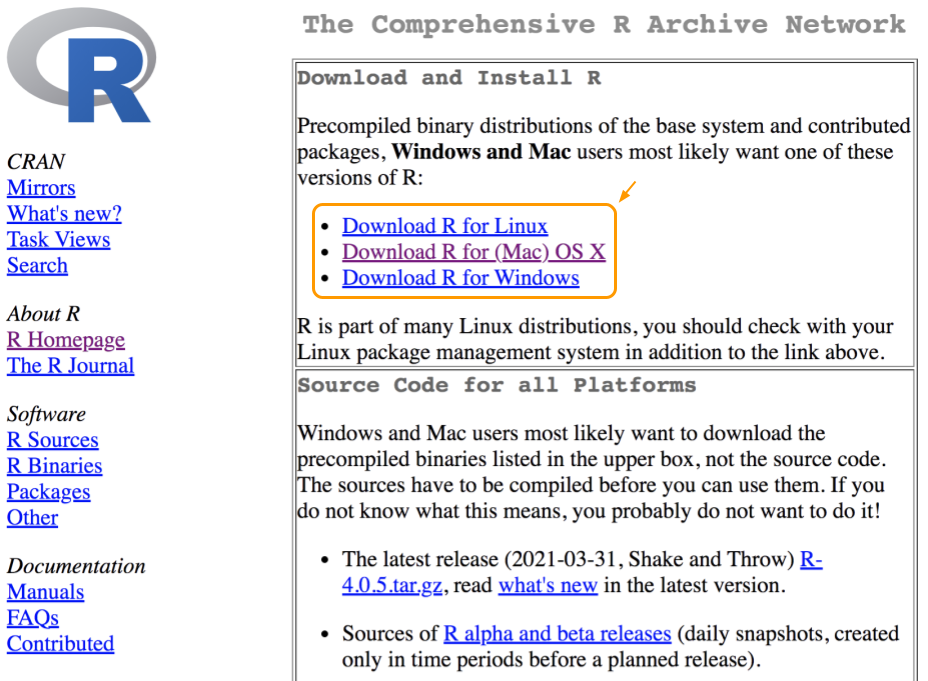
\includegraphics[width=0.7\linewidth]{images/install/cran-download} 

}

\caption{R is available for MacOS, Windows, and Linux}\label{fig:unnamed-chunk-6}
\end{figure}

\textbf{Step 3)} Click on the download option that corresponds to your operating
system (e.g.~Linux, Mac, or Windows). In my case, I have a Mac computer, which
explains why the Mac OS-X link is highlighted in the above screeenshot.

\begin{figure}

{\centering 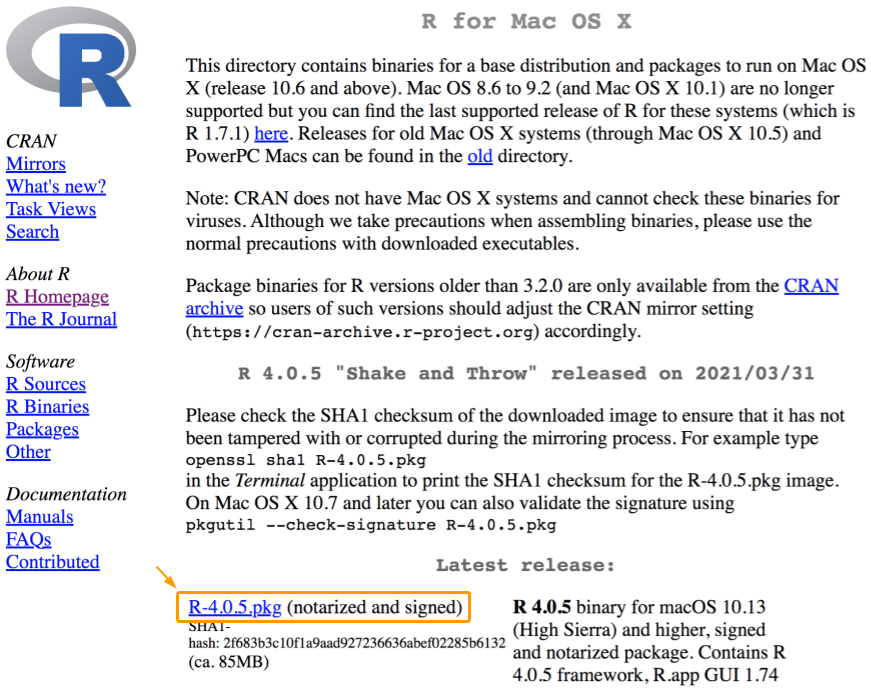
\includegraphics[width=0.7\linewidth]{images/install/cran-mac} 

}

\caption{CRAN download for Mac}\label{fig:unnamed-chunk-7}
\end{figure}

For most users, you will want to install the \textbf{Latest release}, which in the screenshot above happens to be \texttt{R\ 4.0.5\ "Shake\ and\ Throw"}. Keep in mind that
by the time you read this book, R will very likely have a more recent version.

\textbf{Step 4)} Click on the package link, which in the screenshot corresponds to
\texttt{R-4.0.5.pkg}. This is the link of a compressed file that contains the binary
code. Before installing a given version of R, read the
description of the release to make sure the operating system in your computer
is compatible with a specific version of R.

After clicking on the \texttt{R-4.0.5.pkg} link, the compressed file will be
downloaded to your computer.

\textbf{Step 5.} Click on the downloaded file. An installation wizard will open
automatically, ready to guide you through the installation process, step by
step (see image below).

\begin{figure}

{\centering 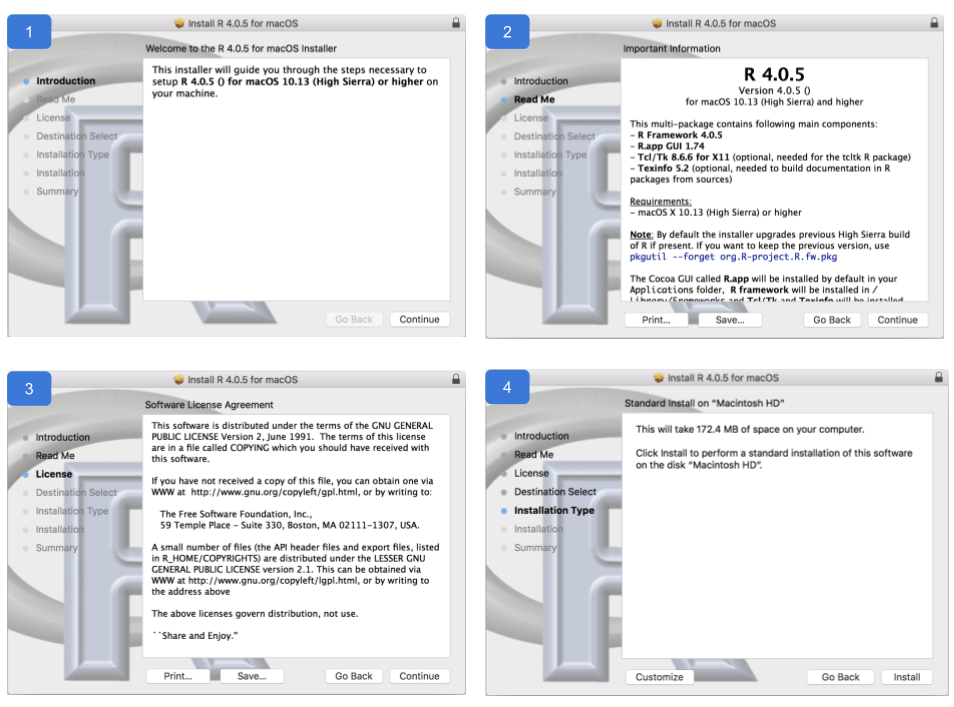
\includegraphics[width=0.9\linewidth]{images/install/R-install-steps} 

}

\caption{R Installation wizard for Mac}\label{fig:unnamed-chunk-8}
\end{figure}

In most cases, you will want to use the default settings. Personally, I've been
using the default settings for several years without having the need to
customize anything.

At the end of the installation, if everything went well, you should be able
to see a successful message (see figure below):

\begin{figure}

{\centering 
\includegraphics[width=0.5\linewidth]{images/install/install-5} 

}

\caption{R Installation wizard for Mac}\label{fig:unnamed-chunk-9}
\end{figure}

\hypertarget{installing-rstudio}{%
\section{Installing RStudio}\label{installing-rstudio}}

In addition to R, the other program you will need to have installed in your
machine is RStudio. To download and install it, follow the steps listed below.

\textbf{Step 1)} Go to \textbf{RStudio's} download webpage:

\url{https://www.rstudio.com/products/rstudio/download/}

\begin{figure}

{\centering 
\includegraphics[width=0.6\linewidth]{images/install/rstudio-download} 

}

\caption{RStudio download options}\label{fig:unnamed-chunk-10}
\end{figure}

At the time of this writing, there are four options of RStudio.

\textbf{Step 2)} Choose the \textbf{free} version of RStudio Desktop (see image below),
and click on the ``DOWNLOAD'' button.

\begin{figure}

{\centering 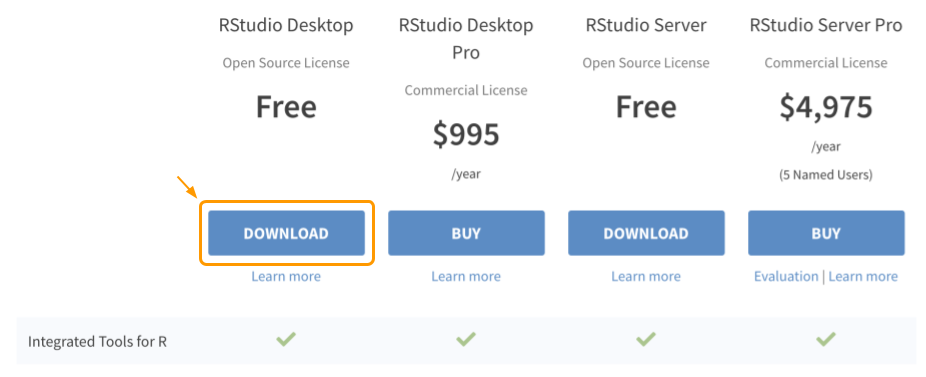
\includegraphics[width=0.6\linewidth]{images/install/rstudio-free} 

}

\caption{Choose RStudio free desktop}\label{fig:unnamed-chunk-11}
\end{figure}

\textbf{Step 3)} Select the version that matches your operating system (e.g.~Windows,
macOS, linux). Double check that the operating system in your computer
is compatible with a specific version of RStudio.

\begin{figure}

{\centering 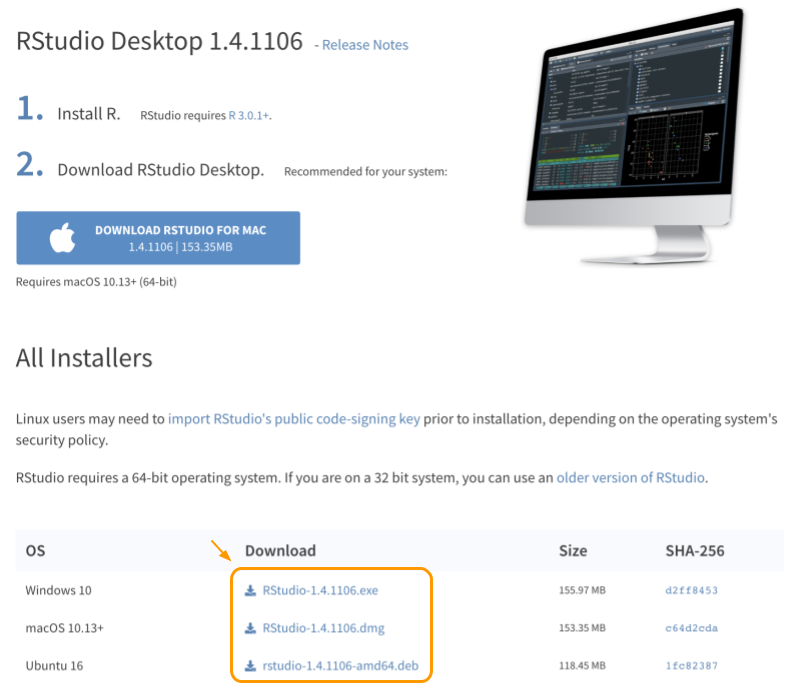
\includegraphics[width=0.6\linewidth]{images/install/rstudio-versions} 

}

\caption{RStudio Desktop versions}\label{fig:unnamed-chunk-12}
\end{figure}

Once the installation of RStudio is completed, you should be able to open a new
session in RStudio, and also to interact with R.

\hypertarget{rintro}{%
\chapter{Breaking the Ice with R}\label{rintro}}

If you are new to R and don't have any programming experience, then you
should read this chapter in its entirety. If you already have some previous
experience working with R and/or have some programming background, then you may
want to skim over most of the introductory chapters of part I.

This chapter, and the rest of the book, assumes that you have installed both R
and RStudio in your computer. If this is not the case, then go to chapter
\protect\hyperlink{install}{Installing R and RStudio} and follow the steps to download
and install these programs.

R comes with a simple built-in graphical user interface (GUI), and you can
certainly start working with it right out of the box. That is actually the way
I got my first contact with R back in 2001 during my senior year in college.
Nowadays, instead of using R's GUI, it is more convenient to interact with R
using a third party software such as RStudio.

I describe more introductory details about RStudio in the next chapter
\protect\hyperlink{rstudio}{A Quick Tour Around RStudio}. For now, go ahead and launch RStudio
in your computer.

\hypertarget{first-contact-with-r-via-rstudio}{%
\section{First Contact with R (via RStudio)}\label{first-contact-with-r-via-rstudio}}

When you open RStudio, you should be able to see its layout organized into
quadrants offically called \emph{panes}. The very first time you launch RStudio you
will only see three panes, like in the screenshot below.

\begin{figure}

{\centering 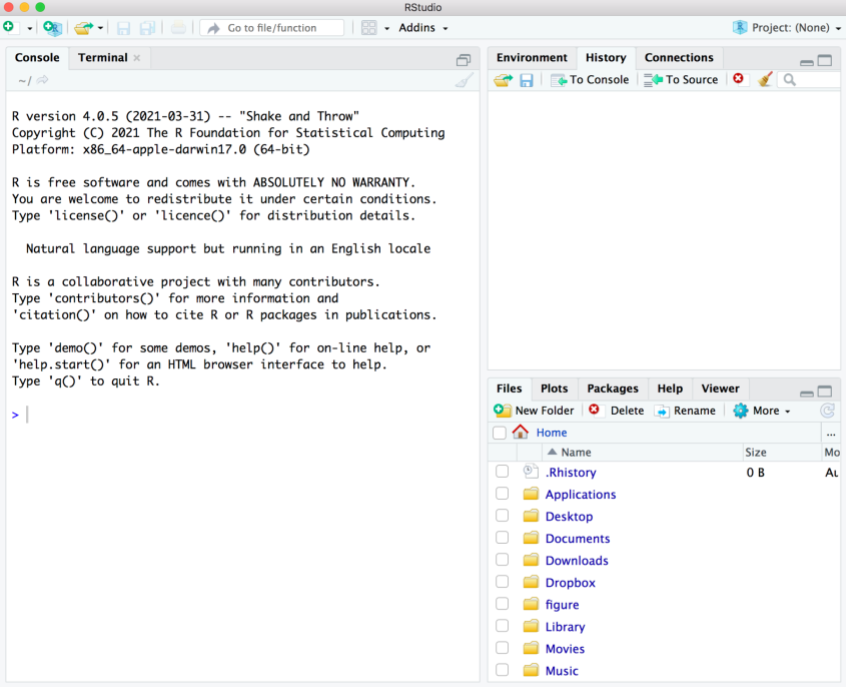
\includegraphics[width=0.7\linewidth]{images/rstudio/rstudio-launch-first-time} 

}

\caption{Screenshot of RStudio when launched for the first time.}\label{fig:unnamed-chunk-14}
\end{figure}

To help you break the ice with R, it's better if we start working directly
on the \textbf{Console}.

As you can tell from the following screenshot, the console is located in the
left-hand side quadrant of RStudio. Keep in mind that your RStudio's console
pane may be located in a different quadrant.

\begin{figure}

{\centering 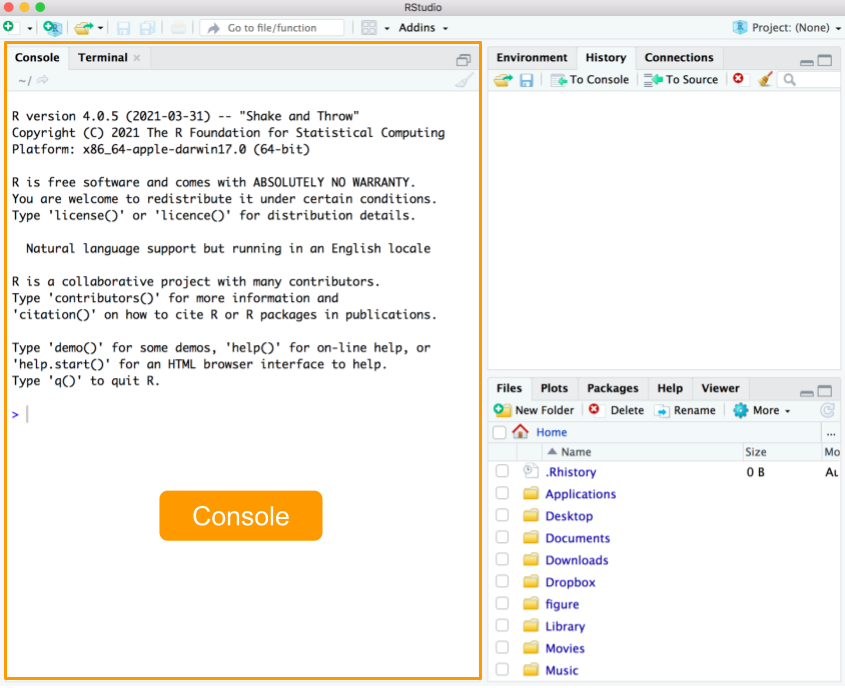
\includegraphics[width=0.7\linewidth]{images/rstudio/rstudio-console-first-time} 

}

\caption{Console quadrant in RStudio.}\label{fig:unnamed-chunk-15}
\end{figure}

Technically speaking, the console is a terminal where a user inputs commands and
views output. Simply put, this is where you can directly interact with R by
typing commands, and getting the output from the execution of the commands.

\hypertarget{r-as-a-scientific-calculator}{%
\subsection{R as a scientific calculator}\label{r-as-a-scientific-calculator}}

This first activity is dedicated for readers with little or no programming
experience, especially those of you who have never used software in which you
have to type commands. The idea is to start typing simple things in the
\textbf{console}, basically using R as a scientific calculator.

Here's a toy example. Consider the monthly bills of an undergraduate student:

\begin{itemize}
\tightlist
\item
  cell phone \$80
\item
  transportation \$20
\item
  groceries \$527
\item
  gym \$10
\item
  rent \$1500
\item
  other \$83
\end{itemize}

You can use R to find the student's total expenses by typing these commands in
the console:

\begin{Shaded}
\begin{Highlighting}[]
\DecValTok{80} \SpecialCharTok{+} \DecValTok{20} \SpecialCharTok{+} \DecValTok{527} \SpecialCharTok{+} \DecValTok{10} \SpecialCharTok{+} \DecValTok{1500} \SpecialCharTok{+} \DecValTok{83}
\end{Highlighting}
\end{Shaded}

There is nothing surprising or fancy about this piece of code. In fact, it has
all the numbers and all the \texttt{+} symbols that you would use if you had to obtain
the total expenses by using the calculator in your cellphone.

\hypertarget{assigning-values-to-objects}{%
\subsection{Assigning values to objects}\label{assigning-values-to-objects}}

Often, it will be more convenient to create \textbf{objects}, sometimes also called
\textbf{variables}, that store one or more values. To do this, type the name of the
object, followed by the assignment or ``arrow'' operator \texttt{\textless{}-}, followed by the
assigned value. By the way, the arrow operator consists of a left-angle bracket
\texttt{\textless{}} (or ``less than'' symbol) and a dash or hyphen symbol \texttt{-}.

For example, you can create an object \texttt{phone} to store the value of the monthly
cell phone bill, and then inspect the object by typing its name:

\begin{Shaded}
\begin{Highlighting}[]
\NormalTok{phone }\OtherTok{\textless{}{-}} \DecValTok{80}
\NormalTok{phone}
\CommentTok{\#\textgreater{} [1] 80}
\end{Highlighting}
\end{Shaded}

All R statements where you create objects are known as \textbf{assignments}, and
they have this form:

\begin{Shaded}
\begin{Highlighting}[]
\NormalTok{object }\OtherTok{\textless{}{-}}\NormalTok{ value}
\end{Highlighting}
\end{Shaded}

this means you assign a \texttt{value} to a given \texttt{object}; one easy way to read the
previous assignment is ``phone gets 80''.

Alternatively, you can also use the equals sign \texttt{=} for assignments:

\begin{Shaded}
\begin{Highlighting}[]
\NormalTok{transportation }\OtherTok{=} \DecValTok{20}
\NormalTok{transportation}
\CommentTok{\#\textgreater{} [1] 20}
\end{Highlighting}
\end{Shaded}

As you will see in the rest of the book, I've written most assignments with the
arrow operator \texttt{\textless{}-}. But you can perfectly replace them with the equals sign
\texttt{=}. The opposite is not necessarily true. There are some especial cases in
which an equals sign cannot be replaced with the arrow, but we'll talk about
this later.

\textbf{Pro tip.} RStudio has a keyboard shortcut for the arrow operator\texttt{\textless{}-}:

\begin{itemize}
\item
  Windows \& Linux users: \texttt{Alt} + \texttt{-}
\item
  Mac users: \texttt{Option} + \texttt{-}
\end{itemize}

In fact, there is a large set of keyboard shortcuts. In the menu bar, go to the
\emph{Help} tab, and then click on the option \emph{Keyboard Shorcuts Help} to find
information about all the available shortcuts.

\hypertarget{object-names}{%
\subsection{Object Names}\label{object-names}}

There are certain rules you have to follow when creating objects and variables.
Object names cannot start with a digit and cannot contain certain other characters
such as a comma or a space.

The following are invalid names (and invalid assignments)

\begin{Shaded}
\begin{Highlighting}[]
\CommentTok{\# cannot start with a number}
\NormalTok{5variable }\OtherTok{\textless{}{-}} \DecValTok{5}

\CommentTok{\# cannot start with an underscore}
\NormalTok{\_invalid }\OtherTok{\textless{}{-}} \DecValTok{10}

\CommentTok{\# cannot contain comma}
\NormalTok{my,variable }\OtherTok{\textless{}{-}} \DecValTok{3}

\CommentTok{\# cannot contain spaces}
\NormalTok{my variable }\OtherTok{\textless{}{-}} \DecValTok{1}
\end{Highlighting}
\end{Shaded}

People use different naming styles, and at some point you should also adopt a
convention for naming things. Some of the common styles are:

\begin{Shaded}
\begin{Highlighting}[]
\NormalTok{snake\_case}

\NormalTok{camelCase}

\NormalTok{period.case}
\end{Highlighting}
\end{Shaded}

Pretty much all the objects and variables that I created in this book follow the
``snake\_case'' style. It is certainly possible that you may endup working with
a team that has a styleguide with a specific naming convention. Feel free to try
various style, and once you feel comfortable with one of them, then stick to it.

\hypertarget{case-sensitive}{%
\subsection{Case Sensitive}\label{case-sensitive}}

R is case sensitive. This means that \texttt{phone} is not the same as \texttt{Phone} or
\texttt{PHONE}

\begin{Shaded}
\begin{Highlighting}[]
\CommentTok{\# case sensitive}
\NormalTok{phone }\OtherTok{\textless{}{-}} \DecValTok{80}
\NormalTok{Phone }\OtherTok{\textless{}{-}} \SpecialCharTok{{-}}\DecValTok{80}
\NormalTok{PHONE }\OtherTok{\textless{}{-}} \DecValTok{8000}

\NormalTok{phone }\SpecialCharTok{+}\NormalTok{ Phone}
\CommentTok{\#\textgreater{} [1] 0}

\NormalTok{PHONE }\SpecialCharTok{{-}}\NormalTok{ phone}
\CommentTok{\#\textgreater{} [1] 7920}
\end{Highlighting}
\end{Shaded}

Again, this is one more reason why adopting a naming convention early on in
a data analysis or programming project is very important. Being consistent with
your notation may save you from some headaches down the road.

\hypertarget{calling-functions}{%
\subsection{Calling Functions}\label{calling-functions}}

Like any other programming language, R has many functions. To use a function
type its name followed by parenthesis. Inside the parenthesis you typically
pass one or more inputs. Most functions will produce some type of output:

\begin{Shaded}
\begin{Highlighting}[]
\CommentTok{\# absolute value}
\FunctionTok{abs}\NormalTok{(}\DecValTok{10}\NormalTok{)}
\FunctionTok{abs}\NormalTok{(}\SpecialCharTok{{-}}\DecValTok{4}\NormalTok{)}

\CommentTok{\# square root}
\FunctionTok{sqrt}\NormalTok{(}\DecValTok{9}\NormalTok{)}

\CommentTok{\# natural logarithm}
\FunctionTok{log}\NormalTok{(}\DecValTok{2}\NormalTok{)}
\end{Highlighting}
\end{Shaded}

In the above examples, the functions are taking a single input. But often you
will be working with functions that accept several inputs. The \texttt{log()} function
is one them. By default, \texttt{log()} computes the natural logarithm. But it also
has the \texttt{base} argument that allows you to specify the base of the logarithm,
say to \texttt{base\ =\ 10}

\begin{Shaded}
\begin{Highlighting}[]
\FunctionTok{log}\NormalTok{(}\DecValTok{10}\NormalTok{, }\AttributeTok{base =} \DecValTok{10}\NormalTok{)}
\CommentTok{\#\textgreater{} [1] 1}
\end{Highlighting}
\end{Shaded}

\hypertarget{comments-in-r}{%
\subsection{Comments in R}\label{comments-in-r}}

All programming languages use a set of characters to indicate that a
specifc part or lines of code are \textbf{comments}, that is, things that are
not to be executed. R uses the hash or pound symbol \texttt{\#} to specify comments.
Any code to the right of \texttt{\#} will not be executed by R.

\begin{Shaded}
\begin{Highlighting}[]
\CommentTok{\# this is a comment}
\CommentTok{\# this is another comment}
\DecValTok{2} \SpecialCharTok{*} \DecValTok{9}

\DecValTok{4} \SpecialCharTok{+} \DecValTok{5}  \CommentTok{\# you can place comments like this}
\end{Highlighting}
\end{Shaded}

You will notice that I have included comments in almost all of the code
snippets shown in the book. To be honest, some examples may have too many
comments, but I've done that to be very explicit, and so that those of you
who lack coding experience understand what's going on. In real life, programmers
use comments, but not so much as I do in the book. The main purpose of
writing comments is to describe---conceptually---what is hapenning with certain
lines of code. Some would even argue that comments should only be used to
express not the what but the \textbf{why} a developer is doing something.

\hypertarget{help-documentation}{%
\section{Getting Help}\label{help-documentation}}

Because we work with functions all the time, it's important to know certain
details about how to use them, what input(s) is required, and what is the
returned output.

So how do you find all this information technically known as \textbf{documentation}?
There are several ways to access this type of information.

If you know the name of a function you are interested in knowing more about,
you can use the function \texttt{help()} and pass it the name of the function you
are looking for:

\begin{Shaded}
\begin{Highlighting}[]
\CommentTok{\# documentation about the \textquotesingle{}abs\textquotesingle{} function}
\FunctionTok{help}\NormalTok{(abs)}

\CommentTok{\# documentation about the \textquotesingle{}mean\textquotesingle{} function}
\FunctionTok{help}\NormalTok{(mean)}
\end{Highlighting}
\end{Shaded}

Alternatively, you can use a shortcut using the question mark \texttt{?} followed
by the name of the function:

\begin{Shaded}
\begin{Highlighting}[]
\CommentTok{\# documentation about the \textquotesingle{}abs\textquotesingle{} function}
\NormalTok{?abs}

\CommentTok{\# documentation about the \textquotesingle{}mean\textquotesingle{} function}
\NormalTok{?mean}
\end{Highlighting}
\end{Shaded}

\texttt{help()} only works if you know the name of the function your are looking for.
Sometimes, however, you don't know the name of the function but you may know
some keyword(s). To look for related functions associated to a keyword, use
\texttt{help.search()} or simply type double question marks \texttt{??}

\begin{Shaded}
\begin{Highlighting}[]
\CommentTok{\# search for \textquotesingle{}absolute\textquotesingle{}}
\FunctionTok{help.search}\NormalTok{(}\StringTok{"absolute"}\NormalTok{)}

\CommentTok{\# alternatively you can also search like this:}
\NormalTok{??absolute}
\end{Highlighting}
\end{Shaded}

Notice the use of quotes surrounding the input name inside \texttt{help.search()}

Often overlooked by beginners but extremely helpful is to understand the
anatomy of the information displayed in the technical documentation. The
content is typical organized into seven sections listed below (although
sometimes you have less or more sections)

\begin{itemize}
\tightlist
\item
  Title
\item
  Description
\item
  Usage of function
\item
  Arguments
\item
  Details
\item
  See Also
\item
  Examples
\end{itemize}

The three screenshots below show the ``Help'' or technical documentation of the
\texttt{log()} function. This information is in RStudio's \texttt{Help} tab, located in the
pane that contains other tabs such as \texttt{Files}, \texttt{Plots}, \texttt{Packages}.

\begin{figure}

{\centering 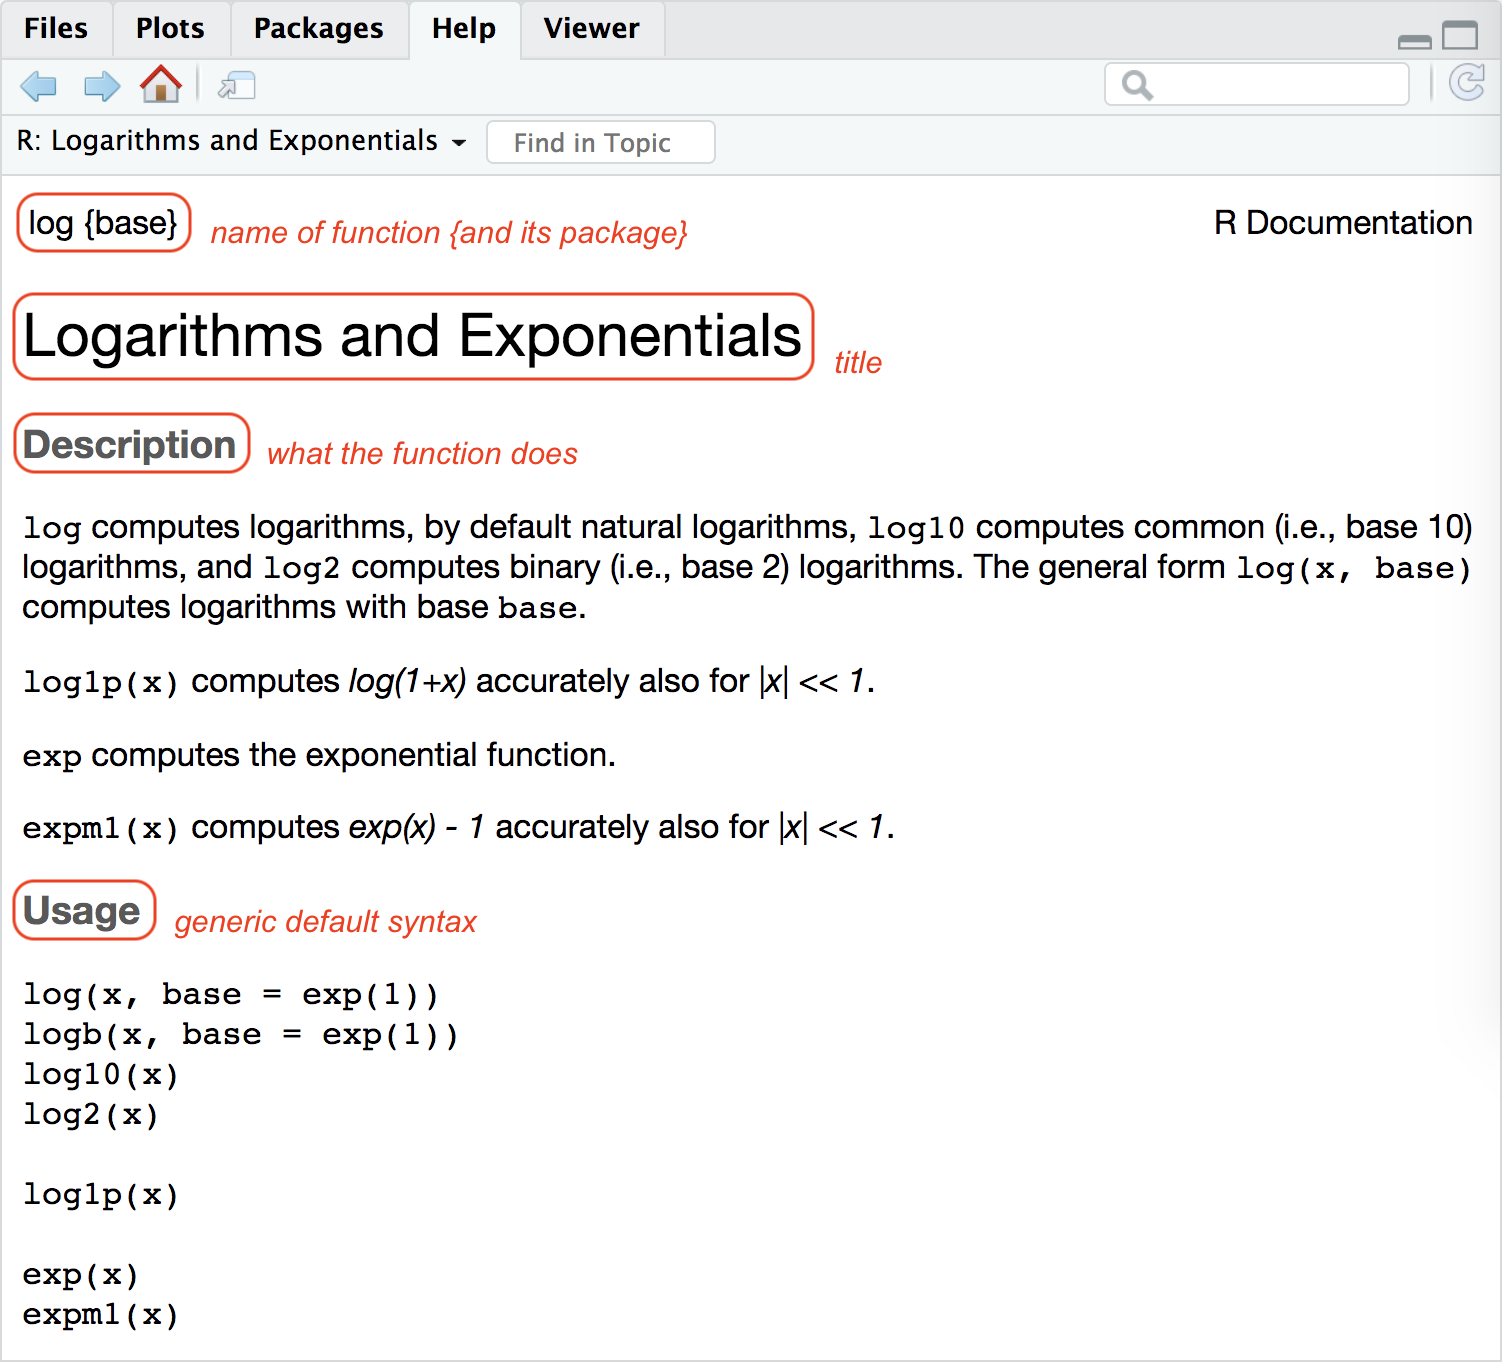
\includegraphics[width=0.8\linewidth]{images/rstudio/help-log-1} 

}

\caption{Help documentation for the log function (part 1)}\label{fig:unnamed-chunk-20}
\end{figure}

\begin{figure}

{\centering 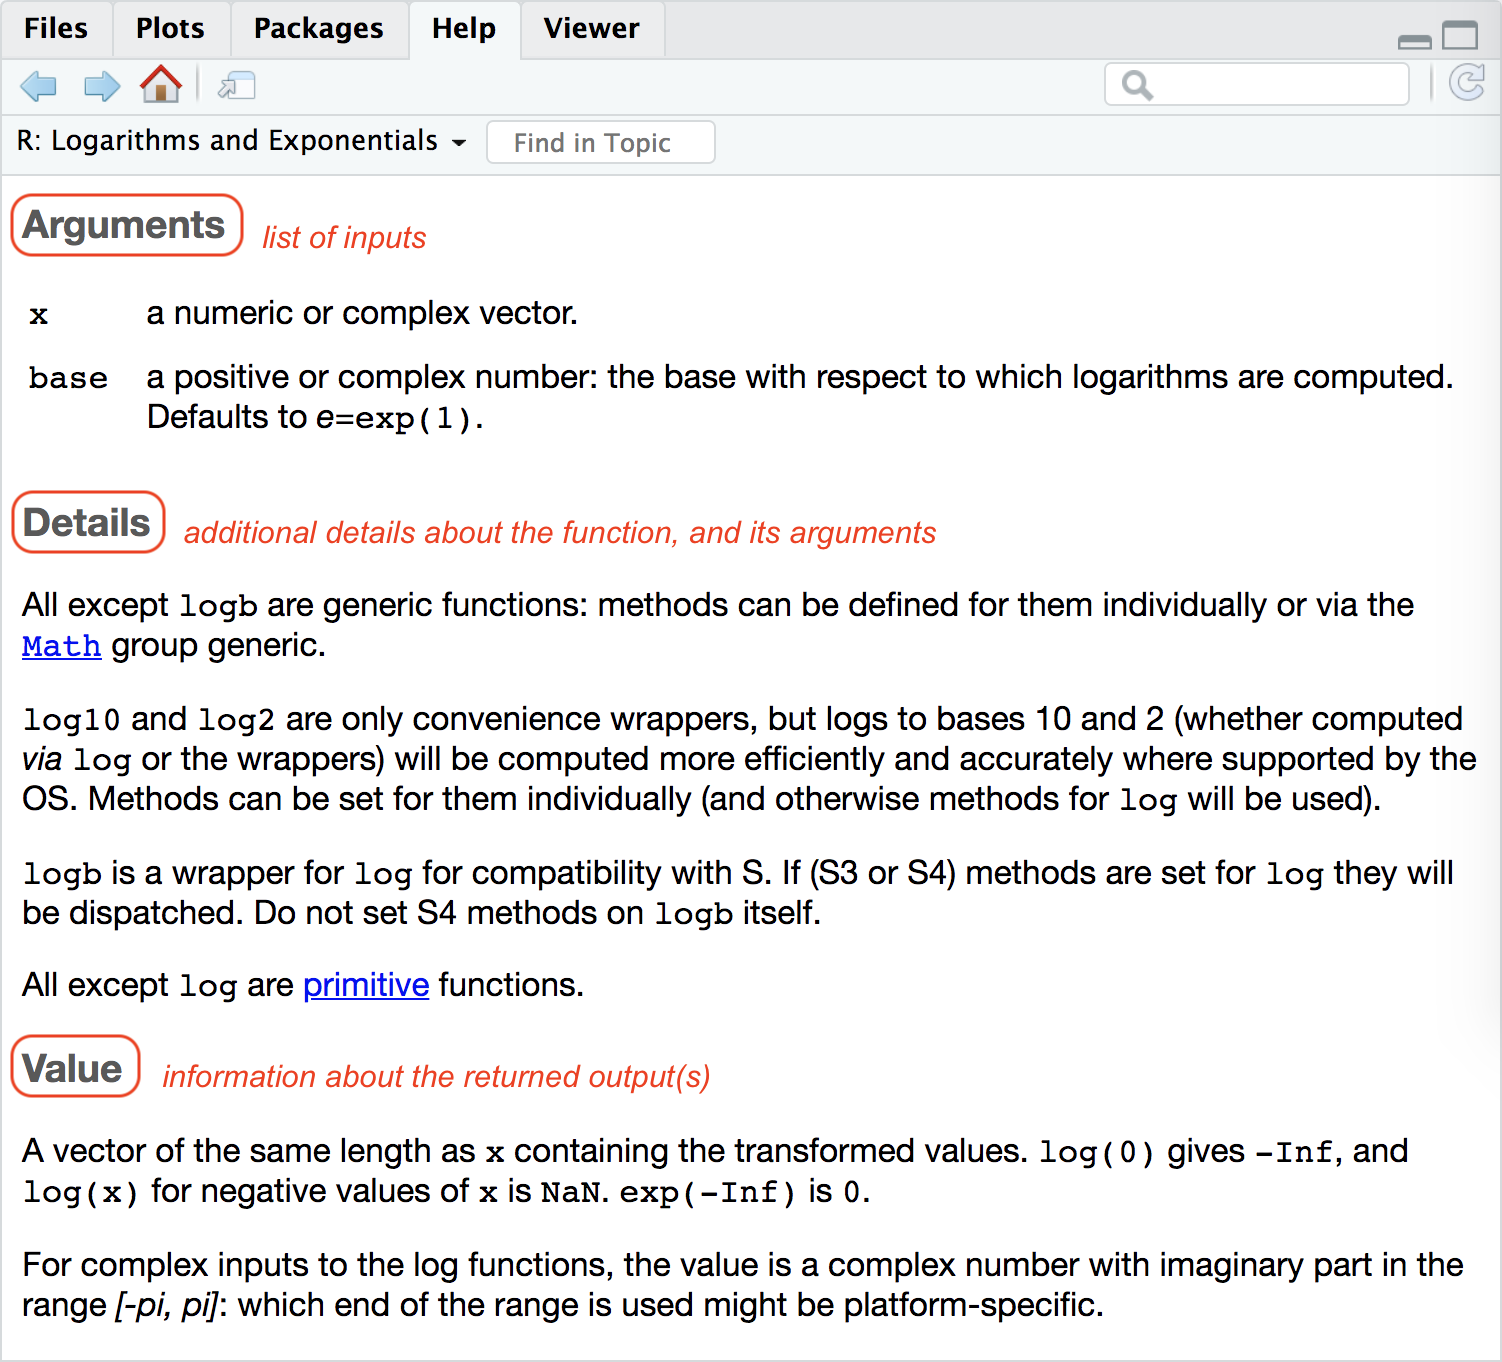
\includegraphics[width=0.8\linewidth]{images/rstudio/help-log-2} 

}

\caption{Help documentation for the log function (part 2)}\label{fig:unnamed-chunk-21}
\end{figure}

\begin{figure}

{\centering 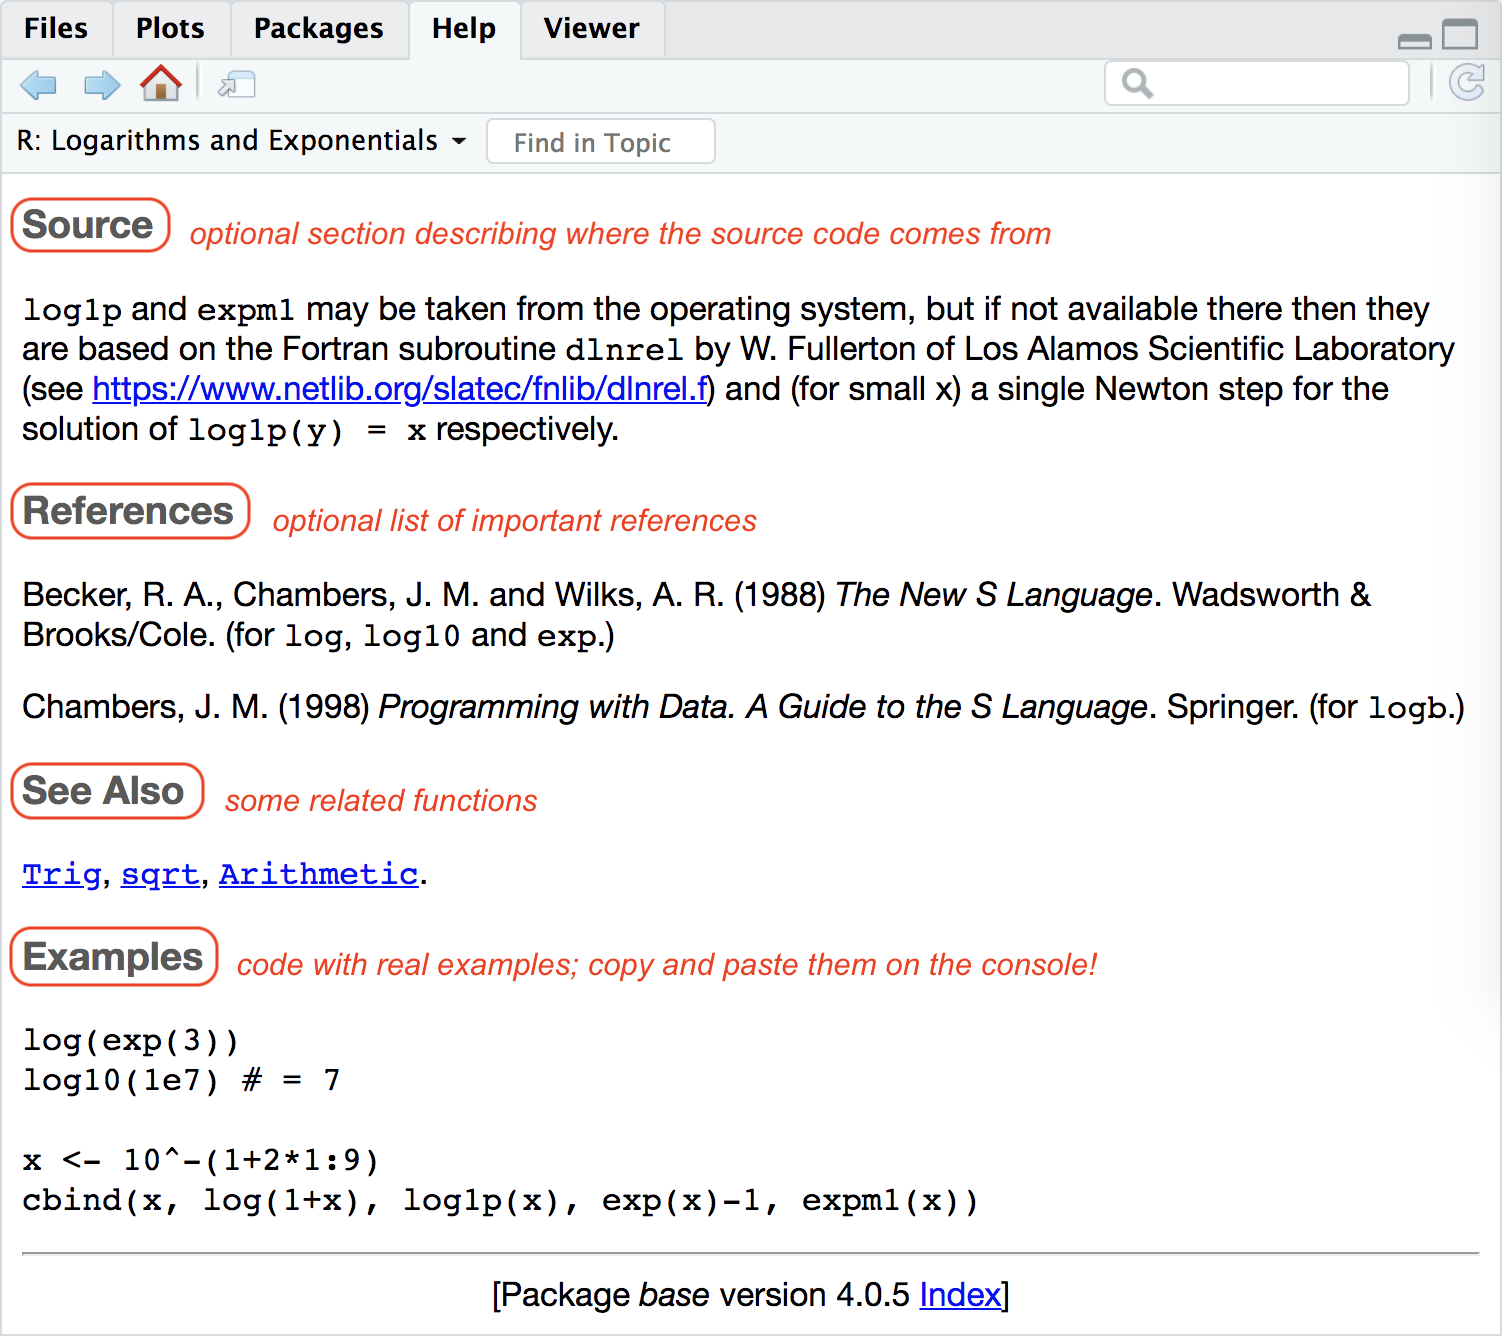
\includegraphics[width=0.8\linewidth]{images/rstudio/help-log-3} 

}

\caption{Help documentation for the log function (part 3)}\label{fig:unnamed-chunk-22}
\end{figure}

\hypertarget{installing-packages}{%
\section{Installing Packages}\label{installing-packages}}

R comes with a large set of functions and packages. A package is a collection
of functions that have been designed for a specific purpose. One of the great
advantages of R is that many analysts, scientists, programmers, and users
can create their own pacakages and make them available for everybody to use them.
R packages can be shared in different ways. The most common way to share a
package is to submit it to what is known as \textbf{CRAN}, the
\emph{Comprehensive R Archive Network}.

You can install a package using the \texttt{install.packages()} function. To do this,
I recommend that you run this command directly on the console. In other words,
do \textbf{not} include this command in a source file (e.g.~\texttt{R} script file, \texttt{Rmd}
file). The reason for running this command directly on the console is to avoid
getting an error message when running code from a source file.

To use \texttt{install.packages()} just give it the name of a package, surrounded by
quotes, and R will look for it in CRAN, and if it finds it, R will download it
to your computer.

\begin{Shaded}
\begin{Highlighting}[]
\CommentTok{\# installing (run this on the console!)}
\FunctionTok{install.packages}\NormalTok{(}\StringTok{"knitr"}\NormalTok{)}
\end{Highlighting}
\end{Shaded}

You can also install a bunch of packages at once by placing their names,
each name separated by a comma, inside the \texttt{c()} function:

\begin{Shaded}
\begin{Highlighting}[]
\CommentTok{\# run this command on the console!}
\FunctionTok{install.packages}\NormalTok{(}\FunctionTok{c}\NormalTok{(}\StringTok{"readr"}\NormalTok{, }\StringTok{"ggplot2"}\NormalTok{))}
\end{Highlighting}
\end{Shaded}

Once you installed a package, you can start using its functions by \emph{loading}
the package with the function \texttt{library()}. For better of worse, \texttt{library()}
allows you to specify the name of the package with or without quotes. Unlike
\texttt{install.packages()} you can only specify the name of one package in \texttt{library()}

\begin{Shaded}
\begin{Highlighting}[]
\CommentTok{\# (this command can be included in an Rmd file)}
\FunctionTok{library}\NormalTok{(knitr)      }\CommentTok{\# without quotes}
\FunctionTok{library}\NormalTok{(}\StringTok{"ggplot2"}\NormalTok{)  }\CommentTok{\# with quotes}
\end{Highlighting}
\end{Shaded}

By the way, you only need to install a package once. After a package has been
installed in your computer, the only command that you need to invoke to use
its functions is the \texttt{library()} function.

\begin{center}\rule{0.5\linewidth}{0.5pt}\end{center}

\hypertarget{exercises}{%
\section{Exercises}\label{exercises}}

\textbf{1)} Here's the list of monthly expenses for a hypothetical undergraduate
student

\begin{itemize}
\tightlist
\item
  cell phone \$80
\item
  transportation \$20
\item
  groceries \$527
\item
  gym \$10
\item
  rent \$1500
\item
  other \$83
\end{itemize}

\begin{enumerate}
\def\labelenumi{\alph{enumi})}
\item
  Using the \texttt{console} pane of RStudio, create objects (i.e.~variables) for each
  of these expenses and create an object \texttt{total} with the sum of the expenses.
\item
  Assuming that the student has the same expenses every month, how much would
  she spend during a school ``semester''? (assume the semester involves five months).
  Write code in R to find this value.
\item
  Maintaining the same assumption about the monthly expenses, how much would she
  spend during a school ``year''? (assume the academic year is 10 months).
  Write code in R to find this value.
\end{enumerate}

\textbf{2)} Use the function \texttt{install.packages()} to install packages \texttt{"stringr"},
\texttt{"RColorBrewer"}, and \texttt{"bookdown"}

\textbf{3)} Use the console to write code for calculating: \(3x^2 + 4x + 8\) when \(x = 2\)

\textbf{4)} Calculate: \(3x^2 + 4x + 8\) but now with a numeric sequence for \(x\)
using \texttt{x\ \textless{}-\ -3:3}

\textbf{5)} Find out how to look for information about math binary operators
like \texttt{+} or \texttt{\^{}} (without using \texttt{?Arithmetic}). \emph{Tip}: quotes are your friend.

\hypertarget{rstudio}{%
\chapter{A Quick Tour Around RStudio}\label{rstudio}}

As I mentioned in the previous chapter, R comes with a simple built-in graphical
user interface, or \emph{GUI} for short. While you can use this interface to
work with R, it is more convenient if you interact with R using a third party
software such as RStudio.

Technically speaking, RStudio is an IDE which is the acronym for
\emph{Integrated Development Environment}. This is just the fancy name for any
software application that provides comprehensive facilities to programmers for
making their lives easier when writing code and developing programs.

Simply put, you can think of RStudio as a ``workbench'' that gives you an
organized working space for interacting with R, while taking care of many of
the little tasks than can be a hassle.

\hypertarget{first-contact-with-rstudio}{%
\section{First Contact with RStudio}\label{first-contact-with-rstudio}}

When you open RStudio, you should be able to see its layout organized into
quadrants officially called \emph{panes} (or panels).

The very first time you launch RStudio you will only see three panes, like in
the screenshot below.

\begin{figure}

{\centering 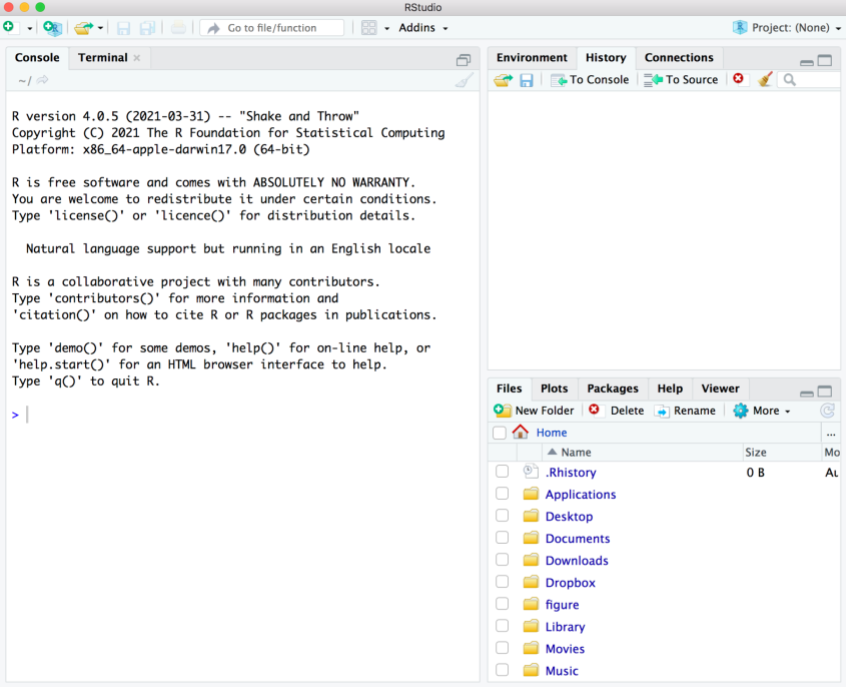
\includegraphics[width=0.7\linewidth]{images/rstudio/rstudio-launch-first-time} 

}

\caption{Screenshot of RStudio when launched for the first time.}\label{fig:unnamed-chunk-24}
\end{figure}

As you can tell from the previous screenshot, the left-hand side shows the
Console pane which is what we used in the previous chapter to write a handful
of simple commands, execute them, and inspect the output provided by R.

If RStudio only displays three panes, why do I call them ``quadrants''? Where is
the fourth pane? Well, to see the extra pane you need to open a file. One
way to do this is by clicking the icon of a blank file with a green plus sign.
This button is located in the top-left corner of the icons menu bar of RStudio.
A drop-down menu with a long list of available file formats will be displayed,
the first option being an ``R Script'' file (see image below).

\begin{figure}

{\centering 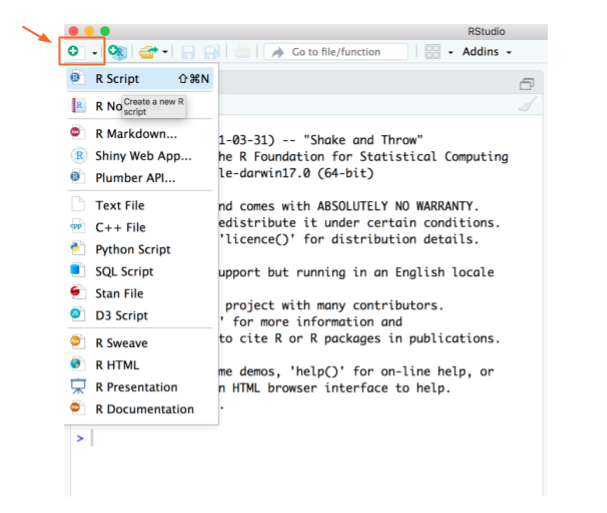
\includegraphics[width=0.6\linewidth]{images/rstudio/rstudio-new-file} 

}

\caption{Opening a new (text) file in RStudio.}\label{fig:unnamed-chunk-25}
\end{figure}

Once you open a (text) file, the layout of RStudio will show the Editor
quadrant, officially called the \emph{Source} pane, like in the following screenshot

\begin{figure}

{\centering 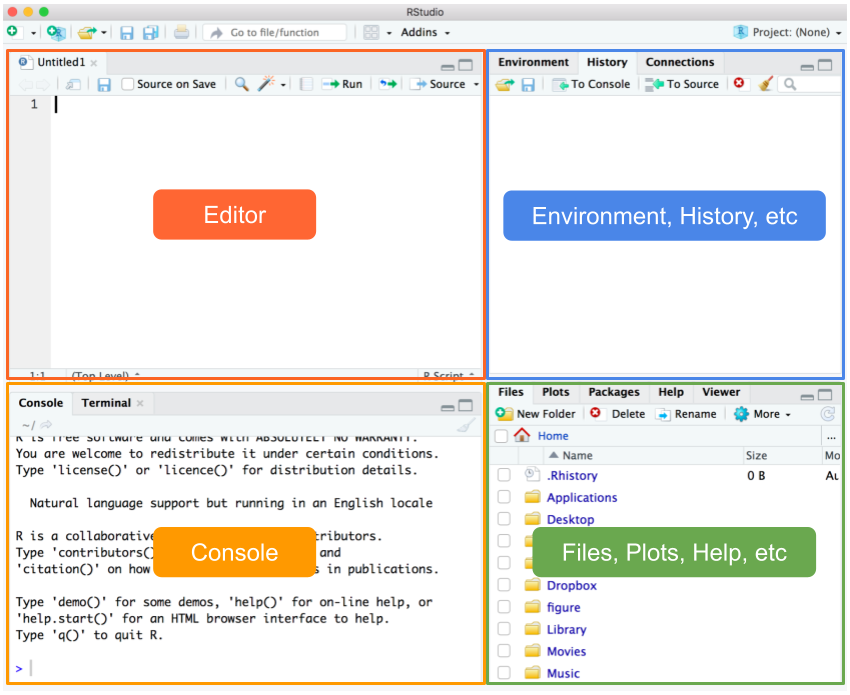
\includegraphics[width=0.8\linewidth]{images/rstudio/rstudio-quadrants} 

}

\caption{RStudio layout organized into quadrants.}\label{fig:unnamed-chunk-26}
\end{figure}

The appearance of RStudio's quadrants can be a bit intimidating for beginners.
But fear not. In the above screenshot, the panes are:

\begin{itemize}
\item
  \texttt{Source} or editor pane (top left quadrant)
\item
  \texttt{Console} pane (bottom left quadrant)
\item
  \texttt{Environment/History/Connections} pane (top right quadrant)
\item
  \texttt{Files/Plots/Packages/Help} pane (bottom right quadrant)
\end{itemize}

\textbf{Pro tip:} you can change the default location of the panes, among many other
things. If you are interested in knowing what customizing options are available,
visit this link for Customizing RStudio

\url{https://support.rstudio.com/hc/en-us/articles/200549016-Customizing-RStudio}

If you have no previous programming experience, you don't have to customize
anything right now. It's better if you wait some days until you get a better
feeling of the working environment. You will probably be experimenting (trial
and error) some time with the customizing options until you find what works for
you.

\hypertarget{rstudio-panes-in-a-nutshell}{%
\section{RStudio Panes in a Nutshell}\label{rstudio-panes-in-a-nutshell}}

Sooner or later you will be using all four panes in RStudio. Most programming
activities will require working with both the \texttt{Source} and \texttt{Console} panes.
Certain operations will involve using the \texttt{Files} tab. Occasionally you will
also use one of the tabs in the \texttt{Environment/History/etc} pane. The set of
specifc tabs that you have to use really depends on the type of work you plan
to carry out. You will have time to learn the basics---and not so basics---of
every pane throughout the book. The more time you spend in RStudio, and the
more you use it, the more features you will discover about it.

\hypertarget{console}{%
\subsection{Console}\label{console}}

The \texttt{Console} is supposed to be the terminal---or the place---where you type in
commands, which R then executes, and where the output of those commands is
typically displayed. The truth is that most programmers don't write commands
\emph{directly} in the console. Instead, what we use is the \texttt{Source} pane to write
commands in a text file (e.g.~an R-Script file, an R-Markdown file), and then
execute the commands from that pane.

The reason for writing commands in a text file and not directly in the console,
is because of convenience and organization. \emph{Convenience} because, as you will
see, many commands involve writing several lines of code which can be tricky to
do it correctly just by typing in the console. \emph{Organization} in the sense that
having all your commands in a text file makes it easy to store your code,
keep track of all the work you do, build upon it, and share it with others.

So, knowing that programmers rarely make direct use of the \texttt{Console}, when
do you actually use this pane? I don't know about the rest of programmers but
I can tell you how I personally use it.

One common use of the \texttt{Console} is when I want to calculate basic things like
the monthly balance in my credit cards, or the overall score for one of the
students in my classes, or some other quick computation. These are types of
calculations that I could perfectly perform with any scientific calculator
like the one in my smartphone. But more often than not I prefer to do them in R,
typically when that's the tool I have at hand (which happens almost every day).

The other typical situation in which I use the console is when I'm trying out
some idea or testing if a certain command could work. I like to explore the
feasibility of my code with a small example in the console, and then refine it
or generalize it by writing code in a text file---using the \texttt{Source} pane.

\hypertarget{files-plots-packages-help}{%
\subsection{Files, Plots, Packages, Help}\label{files-plots-packages-help}}

The \texttt{Files} quadrant contains multiple tabs

\begin{itemize}
\item
  \texttt{Files}: this tab lets you navigate your file system without the need of
  leaving RStudio. You can move to any directory or folder in your home directory,
  inspect the contents of a given folder, create a new folder, and perform
  standard operations on files such as opening, renaming, copying, and deleting.
  In addition, you can also see the working directory, or change it if you want to.
\item
  \texttt{Plots}: this tab is used by R Graphics Devices to display any graphic or
  image produce by an R plotting function.
\item
  \texttt{Packages}: this tab allows you to install and update R packages. Often, you
  will want to use functions from external R packages, and to do this you must
  first install those packages in your system. While it is possible to write
  commands for doing this, the \texttt{Packages} tab gives you a richer interface to
  see what packages are already available in your computer, what their versions
  are, update them if necessary, or delete them in case you no longer need them.
\item
  \texttt{Help}: this is the tab that gives you access to the ``help'' or manual
  documentation of functions, objects, tutorials, and demos of a given R package.
  In the \protect\hyperlink{help-documentation}{previous chapter} we provided an example of the
  manual documentation for the \texttt{log()} function, showing the main anatomy of the
  so-called \emph{R Documentation} files.
\end{itemize}

\hypertarget{source-or-editor}{%
\subsection{Source or Editor}\label{source-or-editor}}

The \texttt{Source} pane is basically the text editor of RStudio. This is the quadrant
you use to edit any text file, again, without the need to leave RStudio.
The reason why is called ``source'' is because the text files edited in this
pane are, for the most part, files that contain the commands that R will
run. In other words, these files are the \textbf{source} of the commands to be
executed.

\hypertarget{environment-history-connections}{%
\subsection{Environment, History, Connections}\label{environment-history-connections}}

The last quadrant is the pane that contains, at least, the following three
tabs: \texttt{Environment}, \texttt{History}, and \texttt{Connections}.

I provide a deeper explanation of the \texttt{Environment} and \texttt{History} tabs in the
following chapter \protect\hyperlink{session}{Session Management}. In the meantime, what you
need to know about \texttt{Environment} is that this tab is used to list the objects
that have being created, or that are available, in a given R session.

In turn, the \texttt{History} tab is a very useful resource that lists \textbf{all} the R
commands that you have executed so far. In theory, R will track all the invoked
commands since the first time you used it, unless you've removed the auxiliary
\texttt{.Rhistory} file linked to your working directory, or unless you've modified
the history mechanism used by your R console.

As for the \texttt{Connections} tab, this plays a more advanced (and somewhat obscure)
role that I briefly discuss in part IV of the book.

\begin{center}\rule{0.5\linewidth}{0.5pt}\end{center}

\hypertarget{exercises-1}{%
\section{Exercises}\label{exercises-1}}

\textbf{1)} In RStudio, one of the panes has tabs \texttt{Files,\ Plots,\ Packages,\ Help,\ Viewer}.

\begin{enumerate}
\def\labelenumi{\alph{enumi})}
\tightlist
\item
  In the tab \textbf{Files}, what happens when you click the button with a House icon?
\item
  Go to the \textbf{Help} tab and search for the documentation of the function \texttt{mean}.
\item
  In the tab \textbf{Help}, what happens when you click the button with a House icon?
\end{enumerate}

\textbf{2)} In RStudio, one of the panes has the tabs \texttt{Environment,\ History,\ Connections}.

\begin{enumerate}
\def\labelenumi{\alph{enumi})}
\tightlist
\item
  If you click on tab \textbf{History}, what do see?
\item
  Find what the buttons of the menu bar in tab \textbf{History} are for.
\item
  Likewise, what can you say about the tab \textbf{Environment}?
\end{enumerate}

\textbf{3)} When you start a new R session in Rstudio, a message with similar content to
the text below appears on the console (the exact content will depend on your
R version):

\begin{verbatim}
   R version 3.5.1 (2018-07-02) -- "Feather Spray"
   Copyright (C) 2018 The R Foundation for Statistical Computing
   Platform: x86_64-apple-darwin15.6.0 (64-bit)

   R is free software and comes with ABSOLUTELY NO WARRANTY.
   You are welcome to redistribute it under certain conditions.
   Type 'license()' or 'licence()' for distribution details.

     Natural language support but running in an English locale   

   R is a collaborative project with many contributors.
   Type 'contributors()' for more information and
   'citation()' on how to cite R or R packages in publications.

   Type 'demo()' for some demos, 'help()' for on-line help, or
   'help.start()' for an HTML browser interface to help.
   Type 'q()' to quit R.
\end{verbatim}

\begin{enumerate}
\def\labelenumi{\alph{enumi})}
\item
  What happens when you type: \texttt{license()}?
\item
  What happens when you type: \texttt{contributors()}?
\item
  What happens when you type: \texttt{citation()}?
\item
  What happens when you type: \texttt{demo()}?
\end{enumerate}

\hypertarget{session}{%
\chapter{Session Management}\label{session}}

In this chapter I review some important aspects about managing your
interactive session with R using RStudio.

From the point of view of a session, all the work, activities, and actions you
do with R can be classified into three categories:

\begin{itemize}
\item
  when starting a session
\item
  during the session
\item
  when closing a session
\end{itemize}

Because there are several things going on behind the scenes in each of the
categories listed above, it is important that we talk about them---at least
briefly.

\hypertarget{starting-a-session}{%
\section{Starting a Session}\label{starting-a-session}}

Starting a session can be done in two primary ways:

\begin{itemize}
\item
  launching the R application program, which will give you access to its
  graphical usier interface; or via RStudio or any other IDE that has the
  ability to open an R session.
\item
  by clicking on a file that your computer associates with R (or RStudio).
  For example, R-script files (with file extension \texttt{.R} or \texttt{.r}), R-Markdown
  files (\texttt{.Rmd} extension), R-Noweb files (\texttt{.Rnw} extension), RStudio project
  files (\texttt{.Rproj} extension), etc.
\end{itemize}

\hypertarget{what-happens-when-you-open-an-r-session-via-rstudio}{%
\subsection{What happens when you open an R session via RStudio?}\label{what-happens-when-you-open-an-r-session-via-rstudio}}

This is an important question that many users never stop to think about.
However, it's worth reviewing what happens when a session is started. So let's
talk about this.

\begin{itemize}
\item
  Every time you open RStudio, the console pane will display R's welcome message.
\item
  The console is always linked to a working directory.
\item
  Typically, the working directory of the console will be your home directory,
  unless you specified a different location when you installed R in your computer.
\item
  You can change the working directory to a different directory if you want.
  This change can be permanent (for future sessions), or temporary (for current
  session).
\item
  To permanently modify working directory (when a session is opened), go to the
  menu bar, select ``RStudio'' tab, click on ``Preferences'', and modify the
  ``R General'' options.
\item
  To temporary change the working directory, go to the menu bar, select the
  ``Session'' tab, and click on ``Set Working Directory'', or simply specify a
  working directory with the \texttt{setwd()} function executed from R's console.
\end{itemize}

\hypertarget{opening-a-session-for-the-first-time}{%
\subsection{Opening a session for the first time}\label{opening-a-session-for-the-first-time}}

If you are opening a session in RStudio for the very fist time:

\begin{itemize}
\item
  the ``Editor'' pane will be collapsed, and
\item
  all the tabs in the ``Environment, History, Connections'' pane will be empty
\end{itemize}

In general, when you open a session (\textbf{not} for the very fist time):

\begin{itemize}
\tightlist
\item
  the ``Environment'' tab may display some objects, which means you have some
  existing objects in your global environment. You can also invoke the list
  function \texttt{ls()} to list any available objects in your current session:
\end{itemize}

\begin{Shaded}
\begin{Highlighting}[]
\CommentTok{\# what objects are in my global environment?}
\FunctionTok{ls}\NormalTok{()}
\end{Highlighting}
\end{Shaded}

\begin{itemize}
\tightlist
\item
  the ``History'' tab may contain lines of previously used commands; if this is
  the case it means that there is an associated a text file called \texttt{.Rhistory} in
  your working directory. You can also use the \texttt{history()} function to display
  the \emph{Commands History}, that is, all the commands invoked in your interactive
  sessions:
\end{itemize}

\begin{Shaded}
\begin{Highlighting}[]
\CommentTok{\# is my history of commands being tracked?}
\FunctionTok{history}\NormalTok{()}
\end{Highlighting}
\end{Shaded}

\hypertarget{working-directory}{%
\subsection{Working Directory}\label{working-directory}}

If you open R via launching an application program (e.g.~RStudio) that lets
you interact with R's console, your session will have an associated working
directory, sometimes also referred to as the \emph{current} working directory.

When you install R in your computer, during the installation process a default
working directory is assigned to R. By default, this directory is your home
directory. You can check whether this is the case if you run the
\emph{get working directory} function \texttt{getwd()} in your console.

\begin{Shaded}
\begin{Highlighting}[]
\CommentTok{\# run this command in the console to find out }
\CommentTok{\# the working directory of your session}
\FunctionTok{getwd}\NormalTok{()}
\end{Highlighting}
\end{Shaded}

In RStudio, you can also look at the console pane, and inspect the text right
below the \texttt{Console} tab that always displays the working directory of your
session. If you see the symbols \texttt{\textasciitilde{}/} it means that the home directory
(represented by the tilde) is your working directory.

\begin{figure}

{\centering 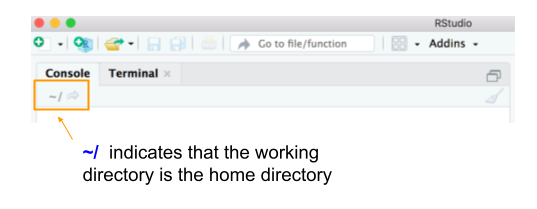
\includegraphics[width=0.7\linewidth]{images/rstudio/rstudio-console-working-directory} 

}

\caption{The working directory is indicated right below the Console tab.}\label{fig:unnamed-chunk-31}
\end{figure}

\hypertarget{working-during-a-session}{%
\section{Working During a Session}\label{working-during-a-session}}

Working with R involves a series of common actions:

\begin{itemize}
\item
  writing commands (on a source document or on the console)
\item
  executing commands (from a source doc or from the console)
\item
  looking or examining outputs
\item
  reading or importing files (e.g.~data files, script files)
\item
  saving or exporting output to files (e.g.~data files, images, results)
\end{itemize}

From the logistical point of vew, it all boils down to executing commands,
taking into account the following:

\begin{itemize}
\item
  where a command is being executed from
\item
  if the command requires an input, where does that input come from?
\item
  if the command produces an output, where does that output go to?
\end{itemize}

This is why we need to describe the following:

\begin{enumerate}
\def\labelenumi{\arabic{enumi}.}
\item
  Working Directory
\item
  Workspace and Global Environment
\item
  History of commands
\end{enumerate}

\hypertarget{working-directory-1}{%
\subsection{Working Directory}\label{working-directory-1}}

You will be writing commands either directly in the console or in a source
document (e.g.~\texttt{R} script file, \texttt{Rmd} file, etc.)

The console is always associated to a working directory (usually your home
directory).

A source document, once it has been saved, will live in some directory.
\textbf{Ideally}, a source document's directory would be used as its working directory,
using relative filepaths to handle all input and output resources required in
thecode of the source document. Unfortunately, this ideal is far from what
happens in practice.

\begin{itemize}
\item
  By default, when you execute code chunks in a \textbf{saved} \texttt{Rmd} file, the
  working directory is the directory where the \texttt{Rmd} file resides in.
\item
  By default, when you execute code from an \texttt{R} file, the working directory
  is that of the console.
\end{itemize}

\hypertarget{workspace-and-global-environment}{%
\subsection{Workspace and Global Environment}\label{workspace-and-global-environment}}

Regardless of where commands are being executed from, R will carry out
all the necessary computations, and objects will be created along the way.

The collection of objects that are being created (\emph{and kept alive}) during a
session are part of what is considered to be your \textbf{workspace}.

At a more technical level, all the objects in your workspace are part of an R
\textbf{environment}. To be more precise, the workspace is the \textbf{Global Environment}.

On the console, if you type \texttt{ls()}, R will display all the available objects
in your workspace.

\begin{Shaded}
\begin{Highlighting}[]
\CommentTok{\# available objects in your workspace}
\FunctionTok{ls}\NormalTok{()}
\end{Highlighting}
\end{Shaded}

You can also go to the pane ``Environment, History, \ldots{}'' and
click on the \texttt{Environment} tab to see the objects in your workspace which are
displayed by default under the option ``Global Environment''.

\hypertarget{commands-history}{%
\subsection{Commands History}\label{commands-history}}

When you start a session, R will track all the commands that you execute during
that session. As you execute commands, they will become part of what is called
the \textbf{Commands History}.

You can find the list of all used commands in the \texttt{History} tab,
located in the \emph{Environment, History, Connections} pane of RStudio. You can
also access the commands history with the function \texttt{history()}.

\begin{figure}

{\centering 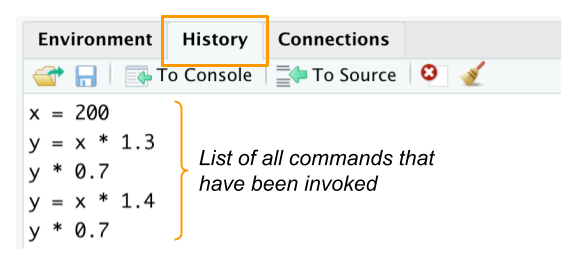
\includegraphics[width=0.65\linewidth]{images/rstudio/rstudio-history-tab} 

}

\caption{The comands history is avaialble in the History tab.}\label{fig:unnamed-chunk-33}
\end{figure}

By default, the history of commands are stored in a text file called \texttt{.Rhistory}
that is saved in your session's working directory.

\hypertarget{closing-a-session}{%
\section{Closing a Session}\label{closing-a-session}}

When closing a session, what should you do?

This is a somewhat ``very personal'' type of question, because it is up to you to
decide what should happen to all the work that you've done in R.

Having said that, you can always decide whether or not to:

\begin{itemize}
\item
  save changes in your source document(s)
\item
  save the commands history in a text file
\item
  save the objects in your workspace (i.e.~objects in Global Environment) in
  a binary file
\end{itemize}

It turns out that RStudio comes with default actions that take place
when you close a session:

\begin{itemize}
\item
  it will ask you if you want to save changes in your source documents
\item
  it will ask you if you want to save the workspace in an \texttt{.RData} file
  (this is a file that uses R's native binary format; this is saved in your
  session's working directory)
\item
  it will automatically save your commands history in a text file called
  \texttt{.Rhistory} (saved in your session's working directory)
\end{itemize}

Also, because of RStudio's default settings, the next time you open a new
session it will:

\begin{itemize}
\item
  restore the previously open source document
\item
  restore objects in the \texttt{.RData} file into your workspace
\item
  give you access to all the commands stored in the \texttt{.Rhistory} file
\end{itemize}

\hypertarget{part-data-objects-in-r}{%
\part{Data Objects in R}\label{part-data-objects-in-r}}

\hypertarget{vectors}{%
\chapter{Vectors}\label{vectors}}

In order to enjoy and exploit R as a computational tool, one of the first
things you need to learn about is the objects R provides to handle data.
The formal name for these programming elements is \textbf{data objects} also known as
\textbf{data structures}. They form the ecosystem of data containers that we can use
to handle various types of data sets, and be able to operate with them in
different forms.

I'm going to use financial math examples as an excuse to introduce and explain
the material. I've found that having a common theme helps avoiding falling
into the ``teaching trap'' of presenting isolated examples in a vacuum.

\hypertarget{motivation-compound-interest}{%
\section{Motivation: Compound Interest}\label{motivation-compound-interest}}

I would like to ask you if you have any of the following accounts:

\begin{itemize}
\item
  Savings account?
\item
  Retirement account?
\item
  Brokerage account?
\end{itemize}

Don't worry if you don't have any of these accounts. I certainly didn't have
any of those accounts until I started my first job right after I finished college.

Anyway, let's consider a hypothetical scenario in which you have \$1000, and
you decide to deposit them in a savings account that pays you an annual
interest rate of 2\%. Assuming that you leave that money in the savings account,
an important question could be:

\begin{quote}
How much money will you have in your savings account \textbf{one} year from now?
\end{quote}

The answer to this question is given by the \textbf{compound interest} formula:

\[
\text{deposit} + \text{paid interest} = \text{amount in one year}
\]

In this example, you deposit \$1000, and the bank pays you 2\% of \$1000 = \$20.
In mathematical terms, we can write the following equation to calculate the
amount that you should expect to have in your savings account within a year:

\[
1000 + 1000 (0.02) = 1000 \times (1 + 0.02) = 1020
\]

You can confirm this by running the following R command:

\begin{Shaded}
\begin{Highlighting}[]
\CommentTok{\# in one year}
\DecValTok{1000} \SpecialCharTok{*}\NormalTok{ (}\FloatTok{1.02}\NormalTok{)}
\CommentTok{\#\textgreater{} [1] 1020}
\end{Highlighting}
\end{Shaded}

Now, if you leave the \$1020 in the savings account for one more year, assuming
that the bank keeps paying you a 2\% annual return, how much money will you have
at the end of the second year?

Well, all you have to do is repeat the same computation, this time by letting
the \$1020---accumulated during the first year---compound for one more year:

\[
1020 + 1020 (0.02) = 1020 \times (1 + 0.02) = 1040.40
\]

which in R can be computed as:

\begin{Shaded}
\begin{Highlighting}[]
\CommentTok{\# in two years}
\DecValTok{1020} \SpecialCharTok{*}\NormalTok{ (}\FloatTok{1.02}\NormalTok{)}
\CommentTok{\#\textgreater{} [1] 1040}
\end{Highlighting}
\end{Shaded}

How much money will you have at the end of three years? Again, take the amount
saved at the end of year 2, and compund it for one more year:

\[
1040.4 + 1040.4 (0.02) = 1040 \times (1 + 0.02) = 1061.208
\]

We can confirm this in R by running the following command:

\begin{Shaded}
\begin{Highlighting}[]
\CommentTok{\# in three years}
\FloatTok{1040.40} \SpecialCharTok{*}\NormalTok{ (}\FloatTok{1.02}\NormalTok{)}
\CommentTok{\#\textgreater{} [1] 1061}
\end{Highlighting}
\end{Shaded}

\hypertarget{creating-objects}{%
\subsection{Creating Objects}\label{creating-objects}}

Often, it will be more convenient to create \textbf{objects} , also referred to as \textbf{variables}, that store both input and output values. To do this, type the
name of the object, followed by the equals sign \texttt{=}, followed by the assigned
value. For example, you can create an object \texttt{d} for the initial deposit of
\$1000, and then inspect the object by typing its name:

\begin{Shaded}
\begin{Highlighting}[]
\CommentTok{\# deposit 1000}
\NormalTok{d }\OtherTok{=} \DecValTok{1000}
\NormalTok{d}
\CommentTok{\#\textgreater{} [1] 1000}
\end{Highlighting}
\end{Shaded}

Alternatively, you can also use the \emph{arrow operator} \texttt{\textless{}-}, technically known as
the \textbf{assignment operator} in R. This operator consists of the left-angle
bracket (i.e.~the less-than symbol) and the dash (i.e.~hyphen character).

\begin{Shaded}
\begin{Highlighting}[]
\CommentTok{\# interest rate of 2\%}
\NormalTok{r }\OtherTok{\textless{}{-}} \FloatTok{0.02}
\NormalTok{r}
\CommentTok{\#\textgreater{} [1] 0.02}
\end{Highlighting}
\end{Shaded}

\hypertarget{assignment-statements}{%
\subsubsection*{Assignment Statements}\label{assignment-statements}}
\addcontentsline{toc}{subsubsection}{Assignment Statements}

All R statements where you create objects are known as ``assignments'', and they
have this form:

\begin{Shaded}
\begin{Highlighting}[]
\NormalTok{object }\OtherTok{\textless{}{-}}\NormalTok{ value}
\end{Highlighting}
\end{Shaded}

this means you assign a \texttt{value} to a given \texttt{object};
you can read the previous assignment as ``r gets 0.02''.

RStudio has a keyboard shortcut for the arrow operator \texttt{\textless{}-}:
\texttt{Alt} + \texttt{-} (the minus sign).

Here are more assignments for each of the savings amounts at the end of years
1, 2, and 3:

\begin{Shaded}
\begin{Highlighting}[]
\CommentTok{\# amounts at the end of years 1, 2, and 3}
\NormalTok{a1 }\OtherTok{=}\NormalTok{ d }\SpecialCharTok{*}\NormalTok{ (}\DecValTok{1} \SpecialCharTok{+}\NormalTok{ r)}
\NormalTok{a2 }\OtherTok{=}\NormalTok{ a1 }\SpecialCharTok{*}\NormalTok{ (}\DecValTok{1} \SpecialCharTok{+}\NormalTok{ r)}
\NormalTok{a3 }\OtherTok{=}\NormalTok{ a2 }\SpecialCharTok{*}\NormalTok{ (}\DecValTok{1} \SpecialCharTok{+}\NormalTok{ r)}
\NormalTok{a3}
\CommentTok{\#\textgreater{} [1] 1061.21}
\end{Highlighting}
\end{Shaded}

\hypertarget{use-descriptive-names}{%
\subsubsection*{Use Descriptive Names}\label{use-descriptive-names}}
\addcontentsline{toc}{subsubsection}{Use Descriptive Names}

While the names of these objects---\texttt{d}, \texttt{r}, \texttt{a1}, etc---are good for a
computer, they can be a bit cryptic for a human being. To be more transparent,
we can use more descriptive names, for example:

\begin{Shaded}
\begin{Highlighting}[]
\CommentTok{\# inputs}
\NormalTok{deposit }\OtherTok{=} \DecValTok{1000}
\NormalTok{rate }\OtherTok{=} \FloatTok{0.02}

\CommentTok{\# amounts at the end of years 1, 2, and 3}
\NormalTok{amount1 }\OtherTok{=}\NormalTok{ deposit }\SpecialCharTok{*}\NormalTok{ (}\DecValTok{1} \SpecialCharTok{+}\NormalTok{ rate)}
\NormalTok{amount2 }\OtherTok{=}\NormalTok{ amount1 }\SpecialCharTok{*}\NormalTok{ (}\DecValTok{1} \SpecialCharTok{+}\NormalTok{ rate)}
\NormalTok{amount3 }\OtherTok{=}\NormalTok{ amount2 }\SpecialCharTok{*}\NormalTok{ (}\DecValTok{1} \SpecialCharTok{+}\NormalTok{ rate)}
\NormalTok{amount3}
\CommentTok{\#\textgreater{} [1] 1061.21}
\end{Highlighting}
\end{Shaded}

The names of the above objects are good for a computer and also for a human
being (that reads English).

Whenever possible, make an effort to use descriptive names. While they don't
matter that much for the computer, they definitely can have a big impact on
any person that takes a look at the code. As it turns out, we tend to spend
more time reviewing and reading code than writing it. So do yourself
(and others) a favor by using descriptive names for your objects.

\hypertarget{combining-various-objects-into-a-single-one}{%
\subsubsection*{Combining various objects into a single one}\label{combining-various-objects-into-a-single-one}}
\addcontentsline{toc}{subsubsection}{Combining various objects into a single one}

We can store various computed values in a single object using the combine or
catenate function \texttt{c()}. Simply list two or more objects inside this function,
separating them by a comma \texttt{,}. Here's an example for how to use \texttt{c()} to
define an object \texttt{amounts} containing the amounts at the end of years 1, 2,
and 3.

\begin{Shaded}
\begin{Highlighting}[]
\CommentTok{\# inputs}
\NormalTok{deposit }\OtherTok{=} \DecValTok{1000}
\NormalTok{rate }\OtherTok{=} \FloatTok{0.02}

\CommentTok{\# amounts at the end of years 1, 2, and 3}
\NormalTok{amount1 }\OtherTok{=}\NormalTok{ deposit }\SpecialCharTok{*}\NormalTok{ (}\DecValTok{1} \SpecialCharTok{+}\NormalTok{ rate)}
\NormalTok{amount2 }\OtherTok{=}\NormalTok{ amount1 }\SpecialCharTok{*}\NormalTok{ (}\DecValTok{1} \SpecialCharTok{+}\NormalTok{ rate)}
\NormalTok{amount3 }\OtherTok{=}\NormalTok{ amount2 }\SpecialCharTok{*}\NormalTok{ (}\DecValTok{1} \SpecialCharTok{+}\NormalTok{ rate)}

\CommentTok{\# combine (catenate) in a single object}
\NormalTok{amounts }\OtherTok{=} \FunctionTok{c}\NormalTok{(amount1, amount2, amount3)}
\NormalTok{amounts}
\CommentTok{\#\textgreater{} [1] 1020.00 1040.40 1061.21}
\end{Highlighting}
\end{Shaded}

So far we have created a bunch of objects. You can use the list function \texttt{ls()}
to display the names of the available objects. But what kind of objects are we
dealing with?

It turns out that all the objects we have so far are \textbf{vectors}.

\hypertarget{about-r-vectors}{%
\section{About R Vectors}\label{about-r-vectors}}

Vectors are the \textbf{most basic} kind of data objects in R. Pretty much all other
R data objects are derived (or are built) from vectors. This is the reason why
I personally like to say that, to a large extent, R is a
\emph{vector-based programming language}.

Based on my own experience, becoming proficient in R requires a solid
understanding of the properties and behavior of R vectors.

To give you a mental picture of what a vector could like, you can think of a
vector as set of contiguous ``cells'' of data, like in the diagram below:

\begin{center}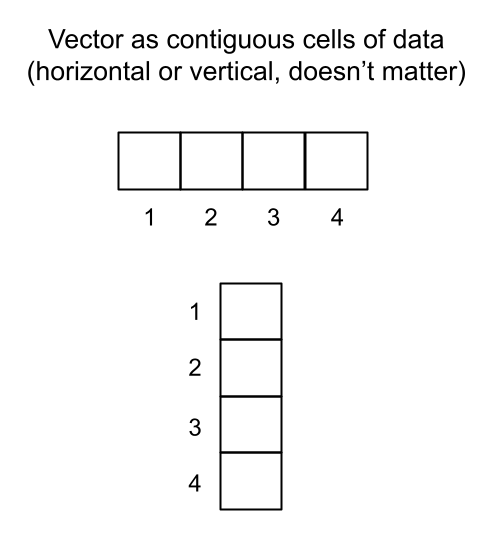
\includegraphics[width=0.4\linewidth]{images/objects/obj-vectors} \end{center}

They can be of any length (including 0), and the starting position or index is
always number 1.

\hypertarget{vectors-are-atomic-objects}{%
\section{Vectors are Atomic Objects}\label{vectors-are-atomic-objects}}

The first thing you should learn about R vectors is that they are consired to
be \textbf{atomic structures}, which is just the fancy name to indicate that all the
elements in a vector are of the \textbf{same type}.

R has four main basic types of atomic vectors:

\begin{itemize}
\tightlist
\item
  \texttt{logical}
\item
  \texttt{integer}
\item
  \texttt{double} or \texttt{real}
\item
  \texttt{character}
\end{itemize}

\begin{center}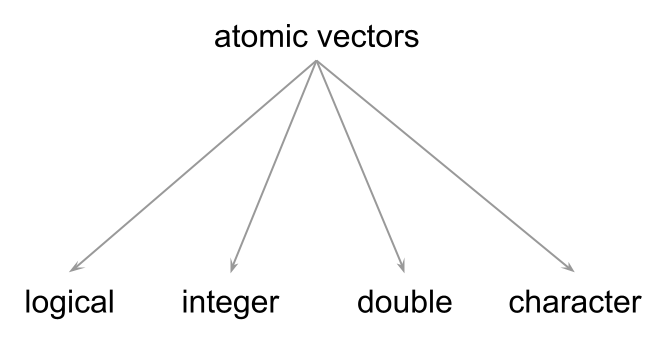
\includegraphics[width=0.55\linewidth]{images/objects/obj-vector-atomic-types} \end{center}

There are also two additional types that are less commonly used: \texttt{complex}
(for complex numbers), and \texttt{raw} which is a binary format used by R.

Here are simple examples of the four common types of vectors:

\begin{Shaded}
\begin{Highlighting}[]
\CommentTok{\# logical}
\NormalTok{a }\OtherTok{=} \ConstantTok{TRUE}

\CommentTok{\# integer}
\NormalTok{x }\OtherTok{=}\NormalTok{ 1L}

\CommentTok{\# double (real)}
\NormalTok{y }\OtherTok{=} \DecValTok{5}

\CommentTok{\# character}
\NormalTok{b }\OtherTok{=} \StringTok{"yosemite"}
\end{Highlighting}
\end{Shaded}

Logical values, known as boolean values in other languages, are \texttt{TRUE} and
\texttt{FALSE}. These values can be abbreviated by using their first letters \texttt{T} and
\texttt{F}, although I discourage you from doing this because it can make code review
a bit harder.

Integer values have an awkward syntax. Notice the appended \texttt{L} when assigning
number 1 to object \texttt{x}. This is not a typo. Rather, this is the syntax used in
R to indicate that a number (with no decimals) is an integer.

If you just simply type a number like \texttt{1} or \texttt{5}, even though cosmetically
they correspond to the mathematical notion of integer numbers, R stores those
numbers as \texttt{double} type. So if you want to declare those numbers as type
\texttt{integer}, you should append an upper case letter \texttt{L} to encode them as \texttt{1L}
and \texttt{5L}.

Character types, referred to as strings in other languages, are specified by
surrounding characters within quotes: either double quotes \texttt{"a"} or single
quotes \texttt{\textquotesingle{}b\textquotesingle{}}. The important thing is to have an opening and a closing quote
of the same kind.

\hypertarget{types-and-modes}{%
\subsection{Types and Modes}\label{types-and-modes}}

How do you know that a given vector is of a certain data type? For better or
worse, there is a couple of functions that allow you to answer this question:

\begin{itemize}
\item
  \texttt{typeof()}
\item
  \texttt{mode()}
\end{itemize}

Although not commonly used within the R community, my recommended function
to determine the data type of a vector is \texttt{typeof()}. The reason for this
recommendation is because \texttt{typeof()} returns the data types previously listed
which are what most other programming languages use:

\begin{Shaded}
\begin{Highlighting}[]
\FunctionTok{typeof}\NormalTok{(deposit)}
\FunctionTok{typeof}\NormalTok{(rate)}
\FunctionTok{typeof}\NormalTok{(amount1)}
\end{Highlighting}
\end{Shaded}

You should know that among the R community, many useRs don't really talk about
\emph{types}. Instead, because of historical reasons related to the S language---on
which R is based---you will often hear useRs talking about \emph{modes} as given by
the \texttt{mode()} function:

\begin{Shaded}
\begin{Highlighting}[]
\FunctionTok{mode}\NormalTok{(deposit)}
\FunctionTok{mode}\NormalTok{(rate)}
\FunctionTok{mode}\NormalTok{(amount1)}
\end{Highlighting}
\end{Shaded}

\texttt{mode()} gives the storage mode of an object, and it actually relies on the
output of \texttt{typeof()}.

When applied to vectors, the main difference between \texttt{mode()} and \texttt{typeof()} is
that \texttt{mode()} groups together types \texttt{"double"} and \texttt{"integer"} into a single
mode called \texttt{"numeric"}.

\begin{figure}

{\centering 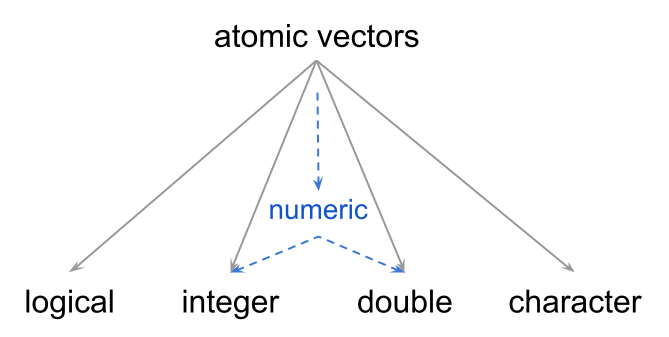
\includegraphics[width=0.55\linewidth]{images/objects/obj-vector-atomic-modes} 

}

\caption{Data types "integer" and "double" correspond to "numeric" mode}\label{fig:unnamed-chunk-48}
\end{figure}

\hypertarget{special-values}{%
\subsection{Special Values}\label{special-values}}

In addition to the four common data types, R also comes with a series of
special values

\begin{itemize}
\item
  \texttt{NULL} is the null object (it has length zero)
\item
  \texttt{NA}, which stands for \emph{Not Available}, indicates a missing value. By default,
  typing \texttt{NA} is stored as a logical value. But there are also special types of
  missing values.

  \begin{itemize}
  \tightlist
  \item
    \texttt{NA\_integer\_}
  \item
    \texttt{NA\_real\_}
  \item
    \texttt{NA\_character\_}
  \end{itemize}
\item
  \texttt{NaN} indicates \emph{Not a Number}. An example of this value is the output
  returned by computing the square root of a negative number: \texttt{sqrt(-5)}
\item
  \texttt{Inf} indicates positive infinite, e.g.~\texttt{100/0}
\item
  \texttt{-Inf} indicates negative infinite, e.g.~\texttt{-100/0}
\end{itemize}

\hypertarget{length-of-vectors}{%
\subsection{Length of Vectors}\label{length-of-vectors}}

The simplest kind of vectors are single values---i.e.~vectors with just one
element. For example, objects such as \texttt{deposit} and \texttt{rate} are one-element
vectors

\begin{Shaded}
\begin{Highlighting}[]
\FunctionTok{length}\NormalTok{(deposit)}
\CommentTok{\#\textgreater{} [1] 1}
\FunctionTok{length}\NormalTok{(rate)}
\CommentTok{\#\textgreater{} [1] 1}
\end{Highlighting}
\end{Shaded}

In most other languages, a number like \texttt{5} or a logical \texttt{TRUE} are usually
considered to be ``scalars''. R, however, does not have the concept of ``scalar'',
instead the simplest data structure is that of a one-element vector.

\hypertarget{creating-vectors}{%
\section{Creating Vectors}\label{creating-vectors}}

We've already seen how to create simple vectors, that is, vectors containing
just one element (i.e.~length-1 vectors)

\begin{Shaded}
\begin{Highlighting}[]
\NormalTok{a }\OtherTok{=} \ConstantTok{TRUE}  \CommentTok{\# logical}
\NormalTok{x }\OtherTok{=}\NormalTok{ 1L    }\CommentTok{\# integer}
\NormalTok{y }\OtherTok{=} \DecValTok{5}     \CommentTok{\# double (real)}
\NormalTok{b }\OtherTok{=} \StringTok{"abc"} \CommentTok{\# character}
\end{Highlighting}
\end{Shaded}

\hypertarget{creating-vectors-with-c}{%
\subsection{\texorpdfstring{Creating vectors with \texttt{c()}}{Creating vectors with c()}}\label{creating-vectors-with-c}}

Among the main functions to work with vectors we have the \textbf{combine} function
\texttt{c()}. This is the workhorse function to create vectors of length greater
than one. Here's how to create a vector \texttt{flavors} with some ice-cream flavors:

\begin{Shaded}
\begin{Highlighting}[]
\NormalTok{flavors }\OtherTok{\textless{}{-}} \FunctionTok{c}\NormalTok{(}\StringTok{\textquotesingle{}lemon\textquotesingle{}}\NormalTok{, }\StringTok{\textquotesingle{}vanilla\textquotesingle{}}\NormalTok{, }\StringTok{\textquotesingle{}chocolate\textquotesingle{}}\NormalTok{)}

\NormalTok{flavors}
\CommentTok{\#\textgreater{} [1] "lemon"     "vanilla"   "chocolate"}
\end{Highlighting}
\end{Shaded}

Basically, you call \texttt{c()} and you type in the values, separating them by
commas.

\hypertarget{numeric-sequences}{%
\subsection{Numeric Sequences}\label{numeric-sequences}}

A common situation when creating vectors involves creating numeric sequences.
If the numeric sequence is short and simple, it could be created with the
combine function \texttt{c()}, for example:

\begin{Shaded}
\begin{Highlighting}[]
\NormalTok{s1 }\OtherTok{=} \FunctionTok{c}\NormalTok{(}\DecValTok{1}\NormalTok{, }\DecValTok{2}\NormalTok{, }\DecValTok{3}\NormalTok{, }\DecValTok{4}\NormalTok{)}
\NormalTok{s1}
\CommentTok{\#\textgreater{} [1] 1 2 3 4}
\end{Highlighting}
\end{Shaded}

Often, you will have to create less simpler and/or longer sequences. For these
purposes there are two useful functions:

\begin{itemize}
\item
  the colon operator \texttt{":"}
\item
  the sequence function \texttt{seq()} and its siblings \texttt{seq.int()}, \texttt{seq\_along()}
  and \texttt{seq.len()}
\end{itemize}

\hypertarget{sequences-with}{%
\subsubsection*{\texorpdfstring{Sequences with \texttt{:}}{Sequences with :}}\label{sequences-with}}
\addcontentsline{toc}{subsubsection}{Sequences with \texttt{:}}

The colon operator \texttt{:} lets you create numeric sequences by indicating the
starting and ending values. For instance, if you want to generate an integer
sequence starting at 1 and ending at 10, you use this command:

\begin{Shaded}
\begin{Highlighting}[]
\NormalTok{ints }\OtherTok{=} \DecValTok{1}\SpecialCharTok{:}\DecValTok{10}
\NormalTok{ints}
\CommentTok{\#\textgreater{}  [1]  1  2  3  4  5  6  7  8  9 10}
\end{Highlighting}
\end{Shaded}

Notice that the the colon operator, when used with whole numbers, will produce
an integer sequence

\begin{Shaded}
\begin{Highlighting}[]
\FunctionTok{typeof}\NormalTok{(ints)}
\CommentTok{\#\textgreater{} [1] "integer"}
\end{Highlighting}
\end{Shaded}

However, when the starting value is not a whole number, then the generated
sequence will be of type \texttt{double}, with unit-steps. For example:

\begin{Shaded}
\begin{Highlighting}[]
\FloatTok{1.5}\SpecialCharTok{:}\FloatTok{5.5}
\CommentTok{\#\textgreater{} [1] 1.5 2.5 3.5 4.5 5.5}
\end{Highlighting}
\end{Shaded}

Run the following commands to see the how R generates different sequences:

\begin{Shaded}
\begin{Highlighting}[]
\FloatTok{1.5}\SpecialCharTok{:}\DecValTok{5}
\FloatTok{1.5}\SpecialCharTok{:}\FloatTok{5.1}
\FloatTok{1.5}\SpecialCharTok{:}\FloatTok{5.5}
\FloatTok{1.5}\SpecialCharTok{:}\FloatTok{5.9}
\end{Highlighting}
\end{Shaded}

You can also create a decreasing sequence by starting with a value on the
left-hand side of \texttt{:} that is greater than the value on the right-hand side:

\begin{Shaded}
\begin{Highlighting}[]
\CommentTok{\# decreasing (reversed) sequence}
\DecValTok{10}\SpecialCharTok{:}\DecValTok{1}
\CommentTok{\#\textgreater{}  [1] 10  9  8  7  6  5  4  3  2  1}
\end{Highlighting}
\end{Shaded}

\hypertarget{sequences-with-seq}{%
\subsubsection*{\texorpdfstring{Sequences with \texttt{seq()}}{Sequences with seq()}}\label{sequences-with-seq}}
\addcontentsline{toc}{subsubsection}{Sequences with \texttt{seq()}}

In addition to the colon operator, R also provides the more generic \texttt{seq()}
function for creating numeric sequences. This function comes with a couple of
parameters that let you generate sequences in various forms.

The simplest usage of \texttt{seq()} involves passing values for the arguments \texttt{from}
(the starting value) and \texttt{to} (the ending value):

\begin{Shaded}
\begin{Highlighting}[]
\CommentTok{\# equivalent to 1:10}
\FunctionTok{seq}\NormalTok{(}\AttributeTok{from =} \DecValTok{1}\NormalTok{, }\AttributeTok{to =} \DecValTok{10}\NormalTok{)}
\CommentTok{\#\textgreater{}  [1]  1  2  3  4  5  6  7  8  9 10}
\end{Highlighting}
\end{Shaded}

As you can tell, the sequence is created with one unit-steps. But this can
be changed with the \texttt{by} argument. Say you want steps of two-units:

\begin{Shaded}
\begin{Highlighting}[]
\FunctionTok{seq}\NormalTok{(}\AttributeTok{from =} \DecValTok{1}\NormalTok{, }\AttributeTok{to =} \DecValTok{10}\NormalTok{, }\AttributeTok{by =} \DecValTok{2}\NormalTok{)}
\CommentTok{\#\textgreater{} [1] 1 3 5 7 9}
\end{Highlighting}
\end{Shaded}

Now, what if you want a decreasing sequence, for example 10, 9, \ldots, 1?
You can also use \texttt{seq()} to achieve this goal. The starting value \texttt{from} is 10,
the ending value \texttt{to} is 1, and the step size \texttt{by} has to be \texttt{-1}

\begin{Shaded}
\begin{Highlighting}[]
\FunctionTok{seq}\NormalTok{(}\AttributeTok{from =} \DecValTok{10}\NormalTok{, }\AttributeTok{to =} \DecValTok{1}\NormalTok{, }\AttributeTok{by =} \SpecialCharTok{{-}}\DecValTok{1}\NormalTok{)}
\CommentTok{\#\textgreater{}  [1] 10  9  8  7  6  5  4  3  2  1}
\end{Highlighting}
\end{Shaded}

Sometimes you may be interested in creating a sequence of a specific length.
When this is the case, you need to use the \texttt{length.out} argument. For example,
say we want to start with 2, getting the sequence of the first six even numbers.
One way to obtain this sequence is with \texttt{from\ =\ 2}, steps of size \texttt{by\ =\ 2},
and a length of \texttt{length.out\ =\ 6}

\begin{Shaded}
\begin{Highlighting}[]
\FunctionTok{seq}\NormalTok{(}\AttributeTok{from =} \DecValTok{2}\NormalTok{, }\AttributeTok{length.out =} \DecValTok{6}\NormalTok{, }\AttributeTok{by =} \DecValTok{2}\NormalTok{)}
\CommentTok{\#\textgreater{} [1]  2  4  6  8 10 12}
\end{Highlighting}
\end{Shaded}

\hypertarget{replicated-vectors}{%
\subsection{Replicated Vectors}\label{replicated-vectors}}

Another interesting function for creating repeated sequences is \texttt{rep()}. This
function takes a vector as the main input, and then it
optionally takes various arguments: \texttt{times}, \texttt{length.out}, and \texttt{each}.

\begin{Shaded}
\begin{Highlighting}[]
\FunctionTok{rep}\NormalTok{(}\DecValTok{1}\NormalTok{, }\AttributeTok{times =} \DecValTok{5}\NormalTok{)        }\CommentTok{\# repeat 1 five times}
\CommentTok{\#\textgreater{} [1] 1 1 1 1 1}
\FunctionTok{rep}\NormalTok{(}\FunctionTok{c}\NormalTok{(}\DecValTok{1}\NormalTok{, }\DecValTok{2}\NormalTok{), }\AttributeTok{times =} \DecValTok{3}\NormalTok{)  }\CommentTok{\# repeat 1 2 three times}
\CommentTok{\#\textgreater{} [1] 1 2 1 2 1 2}
\FunctionTok{rep}\NormalTok{(}\FunctionTok{c}\NormalTok{(}\DecValTok{1}\NormalTok{, }\DecValTok{2}\NormalTok{), }\AttributeTok{each =} \DecValTok{2}\NormalTok{)}
\CommentTok{\#\textgreater{} [1] 1 1 2 2}
\FunctionTok{rep}\NormalTok{(}\FunctionTok{c}\NormalTok{(}\DecValTok{1}\NormalTok{, }\DecValTok{2}\NormalTok{), }\AttributeTok{length.out =} \DecValTok{5}\NormalTok{)}
\CommentTok{\#\textgreater{} [1] 1 2 1 2 1}
\end{Highlighting}
\end{Shaded}

Here are some more complex examples:

\begin{Shaded}
\begin{Highlighting}[]
\FunctionTok{rep}\NormalTok{(}\FunctionTok{c}\NormalTok{(}\DecValTok{3}\NormalTok{, }\DecValTok{2}\NormalTok{, }\DecValTok{1}\NormalTok{), }\AttributeTok{times =} \DecValTok{3}\NormalTok{, }\AttributeTok{each =} \DecValTok{2}\NormalTok{)}
\CommentTok{\#\textgreater{}  [1] 3 3 2 2 1 1 3 3 2 2 1 1 3 3 2 2 1 1}
\end{Highlighting}
\end{Shaded}

\hypertarget{coercion}{%
\section{Coercion}\label{coercion}}

Another fundamental concept that you should learn about vectors is that of
\textbf{coercion}. This has to do with the mechanism that R uses to make sure that
all the elements in a vector are of the same data type.

There are two coercion mechanisms or approaches:

\begin{itemize}
\item
  implicit coercion rules
\item
  explicit coercion functions
\end{itemize}

\hypertarget{implicit-coercion-rules}{%
\subsection{Implicit Coercion Rules}\label{implicit-coercion-rules}}

\textbf{Implicit coercion} is what R does when we try to combine values of different
types into a single vector. Here's an example:

\begin{Shaded}
\begin{Highlighting}[]
\NormalTok{mixed }\OtherTok{\textless{}{-}} \FunctionTok{c}\NormalTok{(}\ConstantTok{TRUE}\NormalTok{, 1L, }\FloatTok{2.0}\NormalTok{, }\StringTok{"three"}\NormalTok{)}
\NormalTok{mixed}
\CommentTok{\#\textgreater{} [1] "TRUE"  "1"     "2"     "three"}
\end{Highlighting}
\end{Shaded}

In this command we are mixing different data types: a logical \texttt{TRUE}, an integer
\texttt{1L}, a double \texttt{2.0}, and a character \texttt{"three"}. Now, even though the input
values are of different data flavors, R has decided to convert everything into
type \texttt{"character"}. Technically speaking, R has \textbf{implicitly coerced} the
values as characters, without asking for our permission and without even
letting us know that it did so.

If you are not familiar with implicit coercion rules, you may get an initial
impression that R is acting weirdly, in a nonsensical form. The more you get
familiar with R, you will notice some interesting coercion patterns. But you
don't need to struggle figuring out what R will do. You just have to remember
the following hierarchy:

\[
\mathsf{character > double > integer > logical}
\]

Here's how R works in terms of coercion:

\begin{itemize}
\item
  characters have priority over other data types: as long as one element is
  a character, all other elements are coerced into characters
\item
  if a vector has numbers (double and integer) and logicals, double will
  dominate
\item
  finally, when mixing integers and logicals, integers will dominate
\end{itemize}

\hypertarget{explicit-coercion-functions}{%
\subsection{Explicit Coercion Functions}\label{explicit-coercion-functions}}

The other type of coercion mechanism, known as \textbf{explicit coercion}, is done
when you explicitly tell R to convert a certain type of vector into a different
data type by using explicit coercion functions:

\begin{itemize}
\tightlist
\item
  \texttt{as.integer()}
\item
  \texttt{as.double()}
\item
  \texttt{as.character()}
\item
  \texttt{as.logical()}
\end{itemize}

Depending on the type of input vector, and the coercion function, you may
achieve what you want, or R may fail to convert things accordingly.

We can take \texttt{deposit}, which is of type double, and convert it into an integer
with no issues:

\begin{Shaded}
\begin{Highlighting}[]
\NormalTok{int\_deposit }\OtherTok{=} \FunctionTok{as.integer}\NormalTok{(deposit)}
\NormalTok{int\_deposit}
\CommentTok{\#\textgreater{} [1] 1000}
\end{Highlighting}
\end{Shaded}

Interestingly, the way an \texttt{integer} number is displayed is exactly the same
as its \texttt{double} version. To confirm that \texttt{int\_deposit} is indeed of type
\texttt{integer} you can use the \texttt{is.integer()} function

\begin{Shaded}
\begin{Highlighting}[]
\FunctionTok{is.integer}\NormalTok{(deposit)}
\CommentTok{\#\textgreater{} [1] FALSE}
\FunctionTok{is.integer}\NormalTok{(int\_deposit)}
\CommentTok{\#\textgreater{} [1] TRUE}
\end{Highlighting}
\end{Shaded}

What about trying to convert a character string such as \texttt{"string"} into an
integer? You can try to apply \texttt{as.integer()} but in this case the attempt is
fruitless:

\begin{Shaded}
\begin{Highlighting}[]
\FunctionTok{as.integer}\NormalTok{(}\StringTok{"string"}\NormalTok{)}
\CommentTok{\#\textgreater{} Warning: NAs introduced by coercion}
\CommentTok{\#\textgreater{} [1] NA}
\end{Highlighting}
\end{Shaded}

\hypertarget{more-about-vectors}{%
\chapter{More About Vectors}\label{more-about-vectors}}

In the previous chapter we started the topic of data objects by introducing
R vectors and some of their basics properties. In this chapter we continue the
discussion of vectors, specifically the notions of vectorization, and
recycling.

\hypertarget{motivation-future-value}{%
\section{Motivation: Future Value}\label{motivation-future-value}}

Let's bring back the savings example from the previous chapter: you have \$1000
and you decide to deposit this money in a savings account that pays you an
annual interest rate of 2\%. We've already seen how to calculate the amount of
money that you would have at the end of the first, second and third years. Let's
now calculate the saved amount for a 10-year period.

\begin{quote}
How much money will you have at the end of each year during a 10-year period?
\end{quote}

To answer this question, we could compute individual amount objects (e.g.~
\texttt{amount1}, \texttt{amount2}, \texttt{amount3}, etc) to get the saved amount at the end of
each year. For example:

\begin{Shaded}
\begin{Highlighting}[]
\CommentTok{\# inputs}
\NormalTok{deposit }\OtherTok{\textless{}{-}} \DecValTok{1000}
\NormalTok{rate }\OtherTok{\textless{}{-}} \FloatTok{0.02}

\CommentTok{\# amounts at the end of years 1, 2, 3, ..., 10}
\NormalTok{amount1 }\OtherTok{=}\NormalTok{ deposit }\SpecialCharTok{*}\NormalTok{ (}\DecValTok{1} \SpecialCharTok{+}\NormalTok{ rate)}
\NormalTok{amount2 }\OtherTok{=}\NormalTok{ amount1 }\SpecialCharTok{*}\NormalTok{ (}\DecValTok{1} \SpecialCharTok{+}\NormalTok{ rate)}
\NormalTok{amount3 }\OtherTok{=}\NormalTok{ amount2 }\SpecialCharTok{*}\NormalTok{ (}\DecValTok{1} \SpecialCharTok{+}\NormalTok{ rate)}
\NormalTok{amount4 }\OtherTok{=}\NormalTok{ amount3 }\SpecialCharTok{*}\NormalTok{ (}\DecValTok{1} \SpecialCharTok{+}\NormalTok{ rate)}
\NormalTok{amount5 }\OtherTok{=}\NormalTok{ amount4 }\SpecialCharTok{*}\NormalTok{ (}\DecValTok{1} \SpecialCharTok{+}\NormalTok{ rate)}
\NormalTok{amount6 }\OtherTok{=}\NormalTok{ amount5 }\SpecialCharTok{*}\NormalTok{ (}\DecValTok{1} \SpecialCharTok{+}\NormalTok{ rate)}
\NormalTok{amount7 }\OtherTok{=}\NormalTok{ amount6 }\SpecialCharTok{*}\NormalTok{ (}\DecValTok{1} \SpecialCharTok{+}\NormalTok{ rate)}
\NormalTok{amount8 }\OtherTok{=}\NormalTok{ amount7 }\SpecialCharTok{*}\NormalTok{ (}\DecValTok{1} \SpecialCharTok{+}\NormalTok{ rate)}
\NormalTok{amount9 }\OtherTok{=}\NormalTok{ amount8 }\SpecialCharTok{*}\NormalTok{ (}\DecValTok{1} \SpecialCharTok{+}\NormalTok{ rate)}
\NormalTok{amount10 }\OtherTok{=}\NormalTok{ amount8 }\SpecialCharTok{*}\NormalTok{ (}\DecValTok{1} \SpecialCharTok{+}\NormalTok{ rate)}
\end{Highlighting}
\end{Shaded}

The problem with this piece of code is that it is too repetitive, time consuming,
boring, and error prone (can you spot the error?). Even worse, imagine if you
were interested in computing the amount of your investment for a 20-year or
a 30-year or a longer year period?

The good news is that we don't have to be so repetitive. Before describing what
the alternative---and more efficient---approach is, we need to do a bit of algebra.

\hypertarget{future-value-formula}{%
\subsection{Future Value Formula}\label{future-value-formula}}

In one year you'll have:

\[
1000 \times (1.02) = 1020
\]

In two years you'll have:

\[
1000 \times (1.02) \times (1.02) = 1000 \times (1.02)^2 = 1040.4
\]

In three years you'll have:

\[
1000 \times (1.02) \times (1.02) \times (1.02) = 1000 \times (1.02)^3 = 1061.208
\]

Do you see a pattern?

If you deposit \$1000 at a rate of return \(r\), how much will you have at the
end of year \(t\)? The answer is given by the Future Value (FV) formula. In its
simplest version, the formula is:

\[
\text{FV} = \text{PV} \times (1 + r)^t
\]

\begin{itemize}
\item
  \(\text{FV}\) = future value (how much you'll have)
\item
  \(\text{PV}\) = present value (the initial deposit)
\item
  \(r\) = rate of return (e.g.~annual rate of return)
\item
  \(t\) = number of periods (e.g.~number of years)
\end{itemize}

Keep in mind that there are more sophisticated versions of the FV formula.
For now, let's keep things simple and use the above equation.

If you deposit \$1000 at a rate of 2\%, how much will you have at the end of
year 10?

\begin{Shaded}
\begin{Highlighting}[]
\NormalTok{deposit }\OtherTok{\textless{}{-}} \DecValTok{1000}
\NormalTok{rate }\OtherTok{\textless{}{-}} \FloatTok{0.02}
\NormalTok{year }\OtherTok{\textless{}{-}} \DecValTok{10}

\NormalTok{amount10 }\OtherTok{\textless{}{-}}\NormalTok{ deposit }\SpecialCharTok{*}\NormalTok{ (}\DecValTok{1} \SpecialCharTok{+}\NormalTok{ rate)}\SpecialCharTok{\^{}}\NormalTok{year}
\NormalTok{amount10}
\CommentTok{\#\textgreater{} [1] 1218.994}
\end{Highlighting}
\end{Shaded}

Using the formula of the Future Value you can directly compute the amount
that you would have at the end of the tenth year. But what about calculating the
amounts at the end of each year during that time period? Enter vectorization!

\hypertarget{vectorization}{%
\section{Vectorization}\label{vectorization}}

In order to explain what vectorization is, let me first show you the following
R code. Compared to the code snippet above, note that the code below uses a
vector \texttt{years} containing a numeric sequence from 1 to 10, thanks to the \texttt{:}
(``colon'') operator. This vector \texttt{years} is then used to play the role of the
exponent in the Future Value formula:

\begin{Shaded}
\begin{Highlighting}[]
\NormalTok{deposit }\OtherTok{\textless{}{-}} \DecValTok{1000}
\NormalTok{rate }\OtherTok{\textless{}{-}} \FloatTok{0.02}
\NormalTok{years }\OtherTok{\textless{}{-}} \DecValTok{1}\SpecialCharTok{:}\DecValTok{10}  \CommentTok{\# vector of years}

\CommentTok{\# example of vectorization (or vectorized code)}
\NormalTok{amounts }\OtherTok{\textless{}{-}}\NormalTok{ deposit }\SpecialCharTok{*}\NormalTok{ (}\DecValTok{1} \SpecialCharTok{+}\NormalTok{ rate)}\SpecialCharTok{\^{}}\NormalTok{years}
\NormalTok{amounts}
\CommentTok{\#\textgreater{}  [1] 1020.000 1040.400 1061.208 1082.432 1104.081 1126.162 1148.686 1171.659}
\CommentTok{\#\textgreater{}  [9] 1195.093 1218.994}
\end{Highlighting}
\end{Shaded}

The computed object \texttt{amounts} is exactly what we are looking for. This vector
contains the saved amounts at the end of each year, from the first year till
the tenth year.

The code used to obtain \texttt{amounts} is an example of one of the most fundamental
and powerful kinds of operations (computations) in R, and it has its special
name: \textbf{vectorization}, also referred to as \textbf{vectorized} code.

When you write code like this:

\begin{Shaded}
\begin{Highlighting}[]
\NormalTok{amounts }\OtherTok{=}\NormalTok{ deposit }\SpecialCharTok{*}\NormalTok{ (}\DecValTok{1} \SpecialCharTok{+}\NormalTok{ rate)}\SpecialCharTok{\^{}}\NormalTok{years}
\end{Highlighting}
\end{Shaded}

we say that your code is \textbf{vectorized}. Technically speaking, this code uses
not just vectorization but it also uses something else called \emph{recycling}, which
we will explain in the next section. But let's describe vectorization first.

\hypertarget{definition-of-vectorization}{%
\subsection{Definition of Vectorization}\label{definition-of-vectorization}}

Simply put, vectorization means that a given function or operation will be
applied to all the elements of one or more vectors, element by element.

Say you want to create a vector \texttt{log\_amounts} by taking the logarithm of
\texttt{amounts}. All you have to do is apply the \texttt{log()} function to \texttt{amounts}:

\begin{Shaded}
\begin{Highlighting}[]
\NormalTok{log\_amounts }\OtherTok{\textless{}{-}} \FunctionTok{log}\NormalTok{(amounts)}
\end{Highlighting}
\end{Shaded}

When you create the vector \texttt{log\_amounts}, what you're doing is applying a
function to a vector, which in turn acts on all the elements of the vector.
Hence the reason why we call it \emph{vectorization} in R parlance.

Most functions that operate with vectors in R are vectorized functions. This
means that an action is applied to all elements of the vector without the need
to explicitly type commands to traverse all of its values, element by element.

In many other programming languages, you would have to use a set of commands
to loop over each element of a vector (or list of numbers) to transform them.
But not in R.

Another simple example of vectorization would be the calculation of the square
root of all the amounts:

\begin{Shaded}
\begin{Highlighting}[]
\FunctionTok{sqrt}\NormalTok{(amounts)}
\end{Highlighting}
\end{Shaded}

\hypertarget{why-should-you-care-about-vectorization}{%
\subsubsection*{Why should you care about vectorization?}\label{why-should-you-care-about-vectorization}}
\addcontentsline{toc}{subsubsection}{Why should you care about vectorization?}

If you are new to programming, learning about R's vectorization will be very
natural and you won't stop to think about it too much. If you have some previous
programming experience in other languages (e.g.~C, python, perl), you know
that vectorization does not tend to be a native thing.

Vectorization is essential in R. It saves you from typing many lines of code,
and you will exploit vectorization with other useful functions known as the
\emph{apply} family functions (we'll talk about them later in the book).

\hypertarget{recycling}{%
\section{Recycling}\label{recycling}}

Closely related with the concept of \emph{vectorization} we have the notion of
\textbf{Recycling}. To explain recycling let's see an example.

The values in the vector \texttt{amounts} are given in dollars, but what if you need
to convert them into values expressed in thousands of dollars?. To convert
from dollars to thousands-of-dollars you just need to divide by 1000; for
example

\begin{itemize}
\tightlist
\item
  1,000 dollars becomes 1 thousands-dollars
\item
  10,000 dollars becomes 10 thousands-dollars
\item
  1 dollar becomes 0.001 thousands-dollars
\end{itemize}

Here is how to create a new vector \texttt{thousands}:

\begin{Shaded}
\begin{Highlighting}[]
\NormalTok{thousands }\OtherTok{\textless{}{-}}\NormalTok{ amounts }\SpecialCharTok{/} \DecValTok{1000}
\NormalTok{thousands}
\CommentTok{\#\textgreater{}  [1] 1.020000 1.040400 1.061208 1.082432 1.104081 1.126162 1.148686 1.171659}
\CommentTok{\#\textgreater{}  [9] 1.195093 1.218994}
\end{Highlighting}
\end{Shaded}

What you just did (assuming that you did things correctly) is called
\textbf{Recycling}, which is what R does when you operate with two (or more) vectors
of \textbf{different length}.

To understand this concept, you need to remember that R does not have a data
structure for scalars (single numbers). Scalars are in reality vectors of
length 1.

The conversion from dollars to thousands-of-dollars requires this operation:
\texttt{amounts\ /\ 1000}. Although it may not be obvious, we are operating with two
vectors of different length: \texttt{amounts} has 10 elements, whereas \texttt{1000} is a
one-element vector. So how does R know what to do in this case?

Well, R uses the \textbf{recycling rule}, which takes the shorter vector (in this
case \texttt{1000}) and recycles its content to form a temporary vector that matches
the length of the longer vector (i.e.~\texttt{amounts}).

\hypertarget{another-recycling-example}{%
\subsubsection*{Another recycling example}\label{another-recycling-example}}
\addcontentsline{toc}{subsubsection}{Another recycling example}

Here's another example of recycling. Saved amounts of elements in an odd
number position will be divided by two; values of elements in an even
number position will be divided by 10:

\begin{Shaded}
\begin{Highlighting}[]
\NormalTok{units }\OtherTok{\textless{}{-}} \FunctionTok{c}\NormalTok{(}\DecValTok{1}\SpecialCharTok{/}\DecValTok{2}\NormalTok{, }\DecValTok{1}\SpecialCharTok{/}\DecValTok{10}\NormalTok{)}
\NormalTok{new\_amounts }\OtherTok{\textless{}{-}}\NormalTok{ amounts }\SpecialCharTok{*}\NormalTok{ units}
\NormalTok{new\_amounts}
\CommentTok{\#\textgreater{}  [1] 510.0000 104.0400 530.6040 108.2432 552.0404 112.6162 574.3428 117.1659}
\CommentTok{\#\textgreater{}  [9] 597.5463 121.8994}
\end{Highlighting}
\end{Shaded}

In this piece of code, the elements of \texttt{units} are recycled (i.e.~repeated) as
many times as the number of elements in \texttt{amounts}.

To achieve the same result without using recycling you would have to create a
vector \texttt{new\_units} (i.e.~the values to divide by) of the same length as \texttt{amounts}.
For example, you could create a vector \texttt{new\_units} with the replicate function
\texttt{rep()} having ten elements in which those values in odd positions are \texttt{1/2}
and those values in even positions are \texttt{1/10}:

\begin{Shaded}
\begin{Highlighting}[]
\NormalTok{new\_units }\OtherTok{\textless{}{-}} \FunctionTok{rep}\NormalTok{(}\FunctionTok{c}\NormalTok{(}\DecValTok{1}\SpecialCharTok{/}\DecValTok{2}\NormalTok{, }\DecValTok{1}\SpecialCharTok{/}\DecValTok{10}\NormalTok{), }\AttributeTok{length.out =} \FunctionTok{length}\NormalTok{(amounts))}
\NormalTok{amounts }\SpecialCharTok{*}\NormalTok{ new\_units}
\CommentTok{\#\textgreater{}  [1] 510.0000 104.0400 530.6040 108.2432 552.0404 112.6162 574.3428 117.1659}
\CommentTok{\#\textgreater{}  [9] 597.5463 121.8994}
\end{Highlighting}
\end{Shaded}

\hypertarget{vectorization-and-recycling}{%
\subsection{Vectorization and Recycling}\label{vectorization-and-recycling}}

Let's bring back the code that uses the Future Value to obtain the vector
\texttt{amounts}:

\begin{Shaded}
\begin{Highlighting}[]
\NormalTok{amounts }\OtherTok{=}\NormalTok{ deposit }\SpecialCharTok{*}\NormalTok{ (}\DecValTok{1} \SpecialCharTok{+}\NormalTok{ rate)}\SpecialCharTok{\^{}}\NormalTok{years}
\end{Highlighting}
\end{Shaded}

Recall that \texttt{deposit} and \texttt{rate} are vectors of length 1. And so it is the
number \texttt{1}, it is a vector containing just one element. In contrast, \texttt{years}
has 10 elements. This means that R is dealing with four vectors some of which
have different lengths.

In pictures, we have the following diagram:

\begin{figure}

{\centering 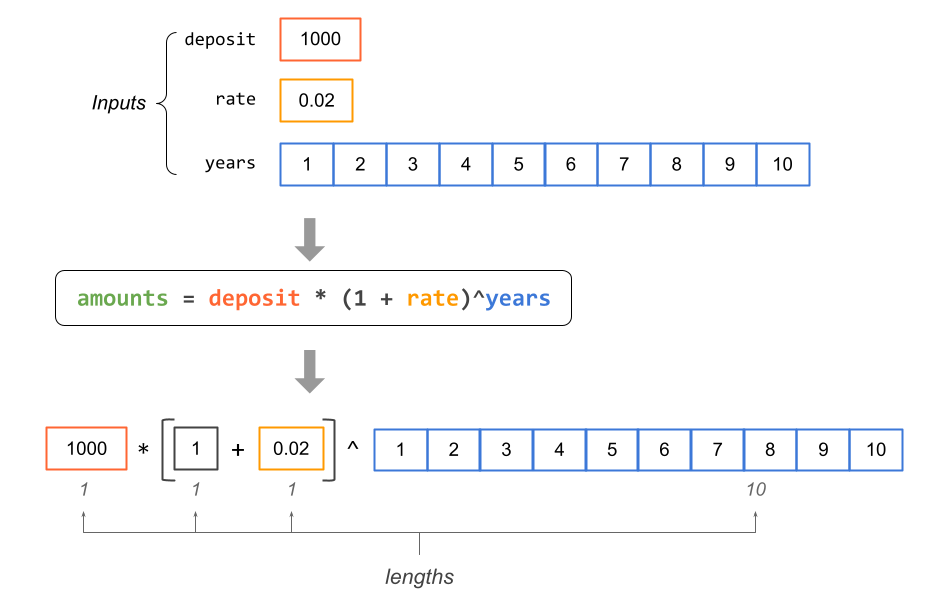
\includegraphics[width=0.9\linewidth]{images/vectors/vectorized1} 

}

\caption{Diagram depicting vectors of different lengths.}\label{fig:unnamed-chunk-76}
\end{figure}

How does R take care of this?

The following diagram depicts what R does behind the scenes: R recycles the
shorter vectors to match the length of the longest vector. In this example,
vectors \texttt{deposit}, \texttt{rate}, and \texttt{1} are the shorter vectors, which are then
recycle to match the length of the longest vector \texttt{years}. The computation
process is completed with vectorization.

\begin{center}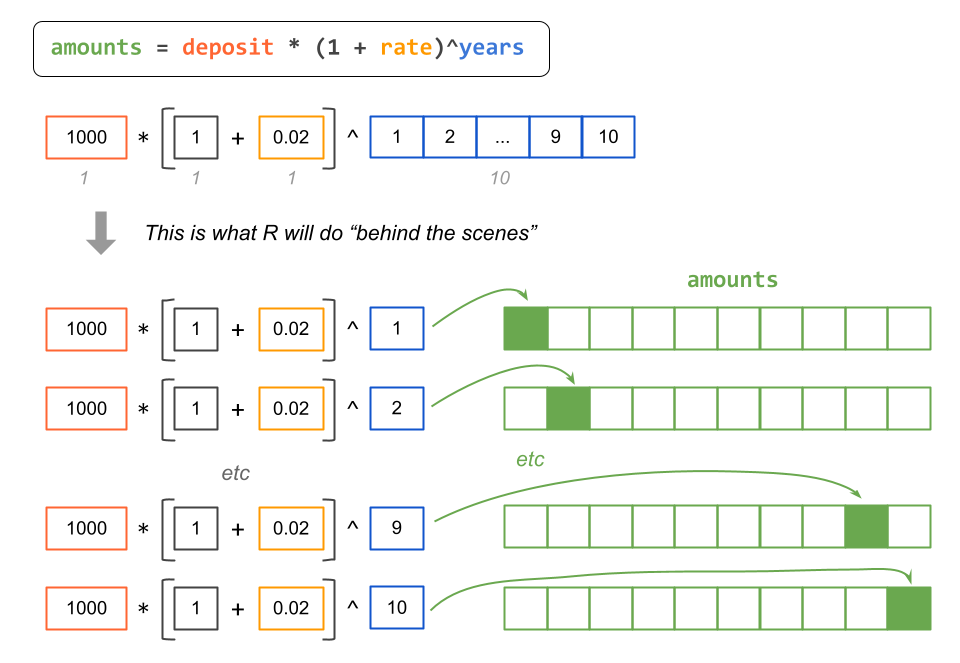
\includegraphics[width=0.9\linewidth]{images/vectors/vectorized2} \end{center}

As you can tell, this is an example of vectorization \& recycling rules in R.

\hypertarget{manipulating-vectors-subsetting}{%
\section{Manipulating Vectors: Subsetting}\label{manipulating-vectors-subsetting}}

In addition to creating vectors, you should also learn how to do some basic
manipulation of vectors. The most common type of manipulation is called
\emph{subsetting}, also known as \emph{indexing} or \emph{subscripting}, which refers to
extracting elements of a vector (or another R object). To do so, you use what
I like to call \textbf{bracket notation}. This implies using (square) brackets \texttt{{[}\ {]}}
to get access to the elements of a vector.

To subset a vector, you type the name of the vector, followed by an opening
and a closing bracket. Inside the brackets you specify

\hypertarget{numeric-subsetting}{%
\subsection{Numeric Subsetting}\label{numeric-subsetting}}

This type of subsetting, as the name indicates, is when the indexing vector
consists of a numeric vector with one or more values that correspond to the position(s) of the vector element(s).

The simplest type of numeric subsetting is when we use single number (which is
a vector of length one).

\begin{Shaded}
\begin{Highlighting}[]
\CommentTok{\# amount at end of year 1}
\NormalTok{amounts[}\DecValTok{1}\NormalTok{]}
\CommentTok{\#\textgreater{} [1] 1020}
\end{Highlighting}
\end{Shaded}

The indexing numeric vector can have more than one element. For example, if
we want to extract the elements in positions 1, 2 and 3, we could provide a
numeric sequence \texttt{1:3}:

\begin{Shaded}
\begin{Highlighting}[]
\CommentTok{\# amounts at end of years 1, 2, and 3}
\NormalTok{amounts[}\DecValTok{1}\SpecialCharTok{:}\DecValTok{3}\NormalTok{]}
\CommentTok{\#\textgreater{} [1] 1020.000 1040.400 1061.208}
\end{Highlighting}
\end{Shaded}

The numeric positions don't have to be consecutive numbers. You can also use
a vector of non-consecutive numbers:

\begin{Shaded}
\begin{Highlighting}[]
\CommentTok{\# amounts at end of years 2 and 4}
\NormalTok{amounts[}\FunctionTok{c}\NormalTok{(}\DecValTok{2}\NormalTok{, }\DecValTok{4}\NormalTok{)]}
\CommentTok{\#\textgreater{} [1] 1040.400 1082.432}
\end{Highlighting}
\end{Shaded}

Likewise, we can also use a vector with repeated numbers:

\begin{Shaded}
\begin{Highlighting}[]
\CommentTok{\# repeated amounts}
\NormalTok{amounts[}\FunctionTok{c}\NormalTok{(}\DecValTok{2}\NormalTok{, }\DecValTok{2}\NormalTok{, }\DecValTok{2}\NormalTok{)]}
\CommentTok{\#\textgreater{} [1] 1040.4 1040.4 1040.4}
\end{Highlighting}
\end{Shaded}

In addition to the previous subscripting options, we can specify negative
numbers to indicate that we want to exclude an element in the associated
position:

\begin{Shaded}
\begin{Highlighting}[]
\CommentTok{\# exclude 2nd year}
\NormalTok{amounts[}\SpecialCharTok{{-}}\DecValTok{2}\NormalTok{]}
\CommentTok{\#\textgreater{} [1] 1020.000 1061.208 1082.432 1104.081 1126.162 1148.686 1171.659 1195.093}
\CommentTok{\#\textgreater{} [9] 1218.994}

\CommentTok{\# exclude 2nd and 4th years}
\NormalTok{amounts[}\SpecialCharTok{{-}}\FunctionTok{c}\NormalTok{(}\DecValTok{2}\NormalTok{, }\DecValTok{4}\NormalTok{)]}
\CommentTok{\#\textgreater{} [1] 1020.000 1061.208 1104.081 1126.162 1148.686 1171.659 1195.093 1218.994}
\end{Highlighting}
\end{Shaded}

\hypertarget{character-subsetting}{%
\subsection{Character Subsetting}\label{character-subsetting}}

Sometimes, you may have a vector with named elements. When this is the case,
you can use a character vector---containing one or more of the element names---as
the indexing vector.

None of the vectors that we have created so far have named elements. So let's
see how to do this. One way to give names to the elements of an existing vector
is with the function \texttt{names()}

\begin{Shaded}
\begin{Highlighting}[]
\NormalTok{amounts3 }\OtherTok{=}\NormalTok{ amounts[}\DecValTok{1}\SpecialCharTok{:}\DecValTok{3}\NormalTok{]}
\FunctionTok{names}\NormalTok{(amounts3) }\OtherTok{=} \FunctionTok{c}\NormalTok{(}\StringTok{"y1"}\NormalTok{, }\StringTok{"y2"}\NormalTok{, }\StringTok{"y3"}\NormalTok{)}
\NormalTok{amounts3}
\CommentTok{\#\textgreater{}       y1       y2       y3 }
\CommentTok{\#\textgreater{} 1020.000 1040.400 1061.208}
\end{Highlighting}
\end{Shaded}

When a vector, like \texttt{amounts3}, has named elements, we can use those names for
subsetting purposes. Instead of using a numeric vector we use a character
vector. Hence the term \emph{character subsetting}.

For example, to extract the element in \texttt{amounts3} that has name \texttt{"y1"} we pass
this string inside the brackets:

\begin{Shaded}
\begin{Highlighting}[]
\NormalTok{amounts3[}\StringTok{"y1"}\NormalTok{]}
\CommentTok{\#\textgreater{}   y1 }
\CommentTok{\#\textgreater{} 1020}
\end{Highlighting}
\end{Shaded}

To get the elements in \texttt{amounts3} that have names \texttt{"y1"} and \texttt{"y3"}, we can
write

\begin{Shaded}
\begin{Highlighting}[]
\NormalTok{amounts3[}\FunctionTok{c}\NormalTok{(}\StringTok{"y1"}\NormalTok{, }\StringTok{"y3"}\NormalTok{)]}
\CommentTok{\#\textgreater{}       y1       y3 }
\CommentTok{\#\textgreater{} 1020.000 1061.208}
\end{Highlighting}
\end{Shaded}

And like in the numeric subsetting case, we can also write a command such as:

\begin{Shaded}
\begin{Highlighting}[]
\NormalTok{amounts3[}\FunctionTok{c}\NormalTok{(}\StringTok{"y2"}\NormalTok{, }\StringTok{"y2"}\NormalTok{, }\StringTok{"y2"}\NormalTok{, }\StringTok{"y1"}\NormalTok{)]}
\CommentTok{\#\textgreater{}     y2     y2     y2     y1 }
\CommentTok{\#\textgreater{} 1040.4 1040.4 1040.4 1020.0}
\end{Highlighting}
\end{Shaded}

\hypertarget{logical-subsetting}{%
\subsection{Logical Subsetting}\label{logical-subsetting}}

Another type of subsetting is when we use a logical vector as the indexing
vector.

Let me show you an example of logical subsetting. In this case, we will use a
logical vector with three elements \texttt{c(TRUE,\ FALSE,\ FALSE)} and pass this
inside the brackets:

\begin{Shaded}
\begin{Highlighting}[]
\NormalTok{amounts3[}\FunctionTok{c}\NormalTok{(}\ConstantTok{TRUE}\NormalTok{, }\ConstantTok{FALSE}\NormalTok{, }\ConstantTok{FALSE}\NormalTok{)]}
\CommentTok{\#\textgreater{}   y1 }
\CommentTok{\#\textgreater{} 1020}
\end{Highlighting}
\end{Shaded}

As you can tell, the retrieved element in \texttt{amounts3} is the one associated to
the \texttt{TRUE} position, whereas those elements associated to the \texttt{FALSE} values
are excluded. This is how the logical values (in the indexing vector) are used:

\begin{itemize}
\tightlist
\item
  \texttt{TRUE} means inclusion
\item
  \texttt{FALSE} means exclusion
\end{itemize}

So, if we want to extract only the element in the second position, we could
write something like this:

\begin{Shaded}
\begin{Highlighting}[]
\NormalTok{amounts3[}\FunctionTok{c}\NormalTok{(}\ConstantTok{FALSE}\NormalTok{, }\ConstantTok{TRUE}\NormalTok{, }\ConstantTok{FALSE}\NormalTok{)]}
\CommentTok{\#\textgreater{}     y2 }
\CommentTok{\#\textgreater{} 1040.4}
\end{Highlighting}
\end{Shaded}

Now, I have to say that doing logical subsetting in this way is not really
how we tend to use it in practice. In other words, we won't be providing an
explicit logical vector, typing a bunch of \texttt{TRUE}'s and \texttt{FALSE}'s values.
Instead, what we typically do is to provide a command that, when executed by R,
will return a logical vector.

Consider the following example. We create a vector \texttt{x}, and then we use the
greater than symbol \texttt{\textgreater{}} to compute a mathematical comparison which in turn
will return a logical vector.

\begin{Shaded}
\begin{Highlighting}[]
\NormalTok{x }\OtherTok{=} \FunctionTok{c}\NormalTok{(}\DecValTok{2}\NormalTok{, }\DecValTok{4}\NormalTok{, }\DecValTok{6}\NormalTok{, }\DecValTok{8}\NormalTok{)}
\NormalTok{x }\SpecialCharTok{\textgreater{}} \DecValTok{5}
\CommentTok{\#\textgreater{} [1] FALSE FALSE  TRUE  TRUE}
\end{Highlighting}
\end{Shaded}

Knowing that \texttt{x\ \textgreater{}\ 5} produces a logical vector in which \texttt{FALSE} indicates that
the number is less than 5, and \texttt{TRUE} indicates that the number
is greater than five, we can write the following command to subset those
elements in \texttt{x} that are greater than five:

\begin{Shaded}
\begin{Highlighting}[]
\NormalTok{x[x }\SpecialCharTok{\textgreater{}} \DecValTok{5}\NormalTok{]}
\CommentTok{\#\textgreater{} [1] 6 8}
\end{Highlighting}
\end{Shaded}

This is a simple example of logical subsetting because the indexing vector
is the logical vector that comes from executing the comparison \texttt{x\ \textgreater{}\ 5}.

Here is a less simple example of logical subsetting to extract the elements in
\texttt{x} that are greater than 3 and less than or equal to 6. This requires\\
two comparison expressions, \texttt{x\ \textgreater{}\ 3} and \texttt{x\ \textless{}=\ 6}, and the use of the logical
\emph{AND} operator \texttt{\&} to form a compound expression:

\begin{Shaded}
\begin{Highlighting}[]
\NormalTok{x[x }\SpecialCharTok{\textgreater{}} \DecValTok{3} \SpecialCharTok{\&}\NormalTok{ x }\SpecialCharTok{\textless{}=} \DecValTok{6}\NormalTok{]}
\CommentTok{\#\textgreater{} [1] 4 6}
\end{Highlighting}
\end{Shaded}

\hypertarget{summary-of-subsetting}{%
\subsection{Summary of Subsetting}\label{summary-of-subsetting}}

In summary, the things that you can specify inside the brackets are three
kind of vectors:

\begin{itemize}
\item
  numeric vectors
\item
  logical vectors (the length of the logical vector must match the length
  of the vector to be subset)
\item
  character vectors (if the elements have names)
\end{itemize}

In addition to the brackets \texttt{{[}{]}}, some common functions that you can use on
vectors are:

\begin{itemize}
\tightlist
\item
  \texttt{length()} gives the number of values
\item
  \texttt{sort()} sorts the values in increasing or decreasing ways
\item
  \texttt{rev()} reverses the values
\item
  \texttt{unique()} extracts unique elements
\end{itemize}

\begin{Shaded}
\begin{Highlighting}[]
\FunctionTok{length}\NormalTok{(amounts3)}
\NormalTok{amounts3[}\FunctionTok{length}\NormalTok{(amounts3)]}
\FunctionTok{sort}\NormalTok{(amounts3, }\AttributeTok{decreasing =} \ConstantTok{TRUE}\NormalTok{)}
\FunctionTok{rev}\NormalTok{(amounts3)}
\end{Highlighting}
\end{Shaded}

\hypertarget{factors}{%
\chapter{Factors}\label{factors}}

I'm one of those with the humble opinion that great software for data science
and analytics should have a data structure dedicated to handle categorical data.
Lucky for us, one of the nicest features about R is that it provides a data
object exclusively designed to handle categorical data: \textbf{factors}.

The term ``factor'' as used in R for handling categorical variables, comes from
the terminology used in \emph{Analysis of Variance}, commonly referred to as ANOVA.
In this statistical method, a categorical variable is commonly referred to as,
surprise-surprise, \emph{factor} and its categories are known as \emph{levels}. Perhaps
this is not the best terminology but it is the one R uses, which reflects its
distinctive statistical origins. Especially for those users without a brackground
in statistics, this is one of R's idiosyncracies that seems disconcerning at
the beginning. But as long as you keep in mind that a factor is just the object
that allows you to handle a qualitative variable you'll be fine. In case you
need it, here's a short mantra to remember:

\begin{quote}
factors have levels
\end{quote}

\hypertarget{creating-factors}{%
\section{Creating Factors}\label{creating-factors}}

To create a factor in R you use the homonym function \texttt{factor()}, which takes a
vector as input. The vector can be either numeric, character or logical. Let's
see our first example:

\begin{Shaded}
\begin{Highlighting}[]
\CommentTok{\# numeric vector}
\NormalTok{num\_vector }\OtherTok{\textless{}{-}} \FunctionTok{c}\NormalTok{(}\DecValTok{1}\NormalTok{, }\DecValTok{2}\NormalTok{, }\DecValTok{3}\NormalTok{, }\DecValTok{1}\NormalTok{, }\DecValTok{2}\NormalTok{, }\DecValTok{3}\NormalTok{, }\DecValTok{2}\NormalTok{)}

\CommentTok{\# creating a factor from num\_vector}
\NormalTok{first\_factor }\OtherTok{\textless{}{-}} \FunctionTok{factor}\NormalTok{(num\_vector)}

\NormalTok{first\_factor}
\CommentTok{\#\textgreater{} [1] 1 2 3 1 2 3 2}
\CommentTok{\#\textgreater{} Levels: 1 2 3}
\end{Highlighting}
\end{Shaded}

As you can tell from the previous code snippet, \texttt{factor()} converts the numeric
vector \texttt{num\_vector} into a factor (i.e.~a categorical variable) with 3
categories---the so called \texttt{levels}.

You can also obtain a factor from a string vector:

\begin{Shaded}
\begin{Highlighting}[]
\CommentTok{\# string vector}
\NormalTok{str\_vector }\OtherTok{\textless{}{-}} \FunctionTok{c}\NormalTok{(}\StringTok{\textquotesingle{}a\textquotesingle{}}\NormalTok{, }\StringTok{\textquotesingle{}b\textquotesingle{}}\NormalTok{, }\StringTok{\textquotesingle{}c\textquotesingle{}}\NormalTok{, }\StringTok{\textquotesingle{}b\textquotesingle{}}\NormalTok{, }\StringTok{\textquotesingle{}c\textquotesingle{}}\NormalTok{, }\StringTok{\textquotesingle{}a\textquotesingle{}}\NormalTok{, }\StringTok{\textquotesingle{}c\textquotesingle{}}\NormalTok{, }\StringTok{\textquotesingle{}b\textquotesingle{}}\NormalTok{)}

\NormalTok{str\_vector}
\CommentTok{\#\textgreater{} [1] "a" "b" "c" "b" "c" "a" "c" "b"}

\CommentTok{\# creating a factor from str\_vector}
\NormalTok{second\_factor }\OtherTok{\textless{}{-}} \FunctionTok{factor}\NormalTok{(str\_vector)}

\NormalTok{second\_factor}
\CommentTok{\#\textgreater{} [1] a b c b c a c b}
\CommentTok{\#\textgreater{} Levels: a b c}
\end{Highlighting}
\end{Shaded}

Notice how \texttt{str\_vector} and \texttt{second\_factor} are displayed. Even though the
elements are the same in both the vector and the factor, they are printed in
different formats. The letters in the string vector are displayed with quotes,
while the letters in the factor are printed without quotes.

And of course, you can use a logical vector to generate a factor as well:

\begin{Shaded}
\begin{Highlighting}[]
\CommentTok{\# logical vector}
\NormalTok{log\_vector }\OtherTok{\textless{}{-}} \FunctionTok{c}\NormalTok{(}\ConstantTok{TRUE}\NormalTok{, }\ConstantTok{FALSE}\NormalTok{, }\ConstantTok{TRUE}\NormalTok{, }\ConstantTok{TRUE}\NormalTok{, }\ConstantTok{FALSE}\NormalTok{)}

\CommentTok{\# creating a factor from log\_vector}
\NormalTok{third\_factor }\OtherTok{\textless{}{-}} \FunctionTok{factor}\NormalTok{(log\_vector)}

\NormalTok{third\_factor}
\CommentTok{\#\textgreater{} [1] TRUE  FALSE TRUE  TRUE  FALSE}
\CommentTok{\#\textgreater{} Levels: FALSE TRUE}
\end{Highlighting}
\end{Shaded}

\hypertarget{how-r-treats-factors}{%
\section{How R treats factors}\label{how-r-treats-factors}}

Technically speaking, R factors are referred to as \emph{compound objects}. According
to the ``R Language Definition'' manual:

\begin{quote}
``Factors are currently implemented using an integer array to specify the
actual levels and a second array of names that are mapped to the integers.''
\end{quote}

What does this mean?

Essentially, a factor is internally stored using two ingredients: one is an
integer vector containing the values of categories, the other is a vector with
the ``levels'' which has the names of categories which are mapped to the integers.

Under the hood, the way R stores factors is as vectors of integer values.
One way to confirm this is using the function \texttt{storage.mode()}

\begin{Shaded}
\begin{Highlighting}[]
\CommentTok{\# storage of factor}
\FunctionTok{storage.mode}\NormalTok{(first\_factor)}
\CommentTok{\#\textgreater{} [1] "integer"}
\end{Highlighting}
\end{Shaded}

This means that we can manipulate factors just like we manipulate vectors. In
addition, many functions for vectors can be applied to factors. For instance,
we can use the function \texttt{length()} to get the number of elements in a factor:

\begin{Shaded}
\begin{Highlighting}[]
\CommentTok{\# factors have length}
\FunctionTok{length}\NormalTok{(first\_factor)}
\CommentTok{\#\textgreater{} [1] 7}
\end{Highlighting}
\end{Shaded}

We can also use the square brackets \texttt{{[}\ {]}} to extract or select elements of a
factor. Inside the brackets we specify vectors of indices such as numeric
vectors, logical vectors, and sometimes even character vectors.

\begin{Shaded}
\begin{Highlighting}[]
\CommentTok{\# first element}
\NormalTok{first\_factor[}\DecValTok{1}\NormalTok{]}

\CommentTok{\# third element}
\NormalTok{first\_factor[}\DecValTok{3}\NormalTok{]}

\CommentTok{\# second to fourth elements}
\NormalTok{first\_factor[}\DecValTok{2}\SpecialCharTok{:}\DecValTok{4}\NormalTok{]}

\CommentTok{\# last element}
\NormalTok{first\_factor[}\FunctionTok{length}\NormalTok{(first\_factor)]}

\CommentTok{\# logical subsetting}
\NormalTok{first\_factor[}\FunctionTok{rep}\NormalTok{(}\FunctionTok{c}\NormalTok{(}\ConstantTok{TRUE}\NormalTok{, }\ConstantTok{FALSE}\NormalTok{), }\AttributeTok{length.out =} \DecValTok{7}\NormalTok{)]}
\end{Highlighting}
\end{Shaded}

If you have a factor with named elements, you can also specify the names of
the elements within the brackets:

\begin{Shaded}
\begin{Highlighting}[]
\FunctionTok{names}\NormalTok{(first\_factor) }\OtherTok{\textless{}{-}}\NormalTok{ letters[}\DecValTok{1}\SpecialCharTok{:}\FunctionTok{length}\NormalTok{(first\_factor)]}
\NormalTok{first\_factor}
\CommentTok{\#\textgreater{} a b c d e f g }
\CommentTok{\#\textgreater{} 1 2 3 1 2 3 2 }
\CommentTok{\#\textgreater{} Levels: 1 2 3}

\NormalTok{first\_factor[}\FunctionTok{c}\NormalTok{(}\StringTok{\textquotesingle{}b\textquotesingle{}}\NormalTok{, }\StringTok{\textquotesingle{}d\textquotesingle{}}\NormalTok{, }\StringTok{\textquotesingle{}f\textquotesingle{}}\NormalTok{)]}
\CommentTok{\#\textgreater{} b d f }
\CommentTok{\#\textgreater{} 2 1 3 }
\CommentTok{\#\textgreater{} Levels: 1 2 3}
\end{Highlighting}
\end{Shaded}

However, you should know that factors are NOT really vectors. To see this you
can check the behavior of the functions \texttt{is.factor()} and \texttt{is.vector()} on a
factor:

\begin{Shaded}
\begin{Highlighting}[]
\CommentTok{\# factors are not vectors}
\FunctionTok{is.vector}\NormalTok{(first\_factor)}
\CommentTok{\#\textgreater{} [1] FALSE}

\CommentTok{\# factors are factors}
\FunctionTok{is.factor}\NormalTok{(first\_factor)}
\CommentTok{\#\textgreater{} [1] TRUE}
\end{Highlighting}
\end{Shaded}

Even a single element of a factor is also a factor:

\begin{Shaded}
\begin{Highlighting}[]
\FunctionTok{class}\NormalTok{(first\_factor[}\DecValTok{1}\NormalTok{])}
\CommentTok{\#\textgreater{} [1] "factor"}
\end{Highlighting}
\end{Shaded}

\hypertarget{so-what-makes-a-factor-different-from-a-vector}{%
\subsubsection*{So what makes a factor different from a vector?}\label{so-what-makes-a-factor-different-from-a-vector}}
\addcontentsline{toc}{subsubsection}{So what makes a factor different from a vector?}

Well, it turns out that factors have an additional attribute that vectors don't:
\texttt{levels}. And as you can expect, the class of a factor is indeed \texttt{"factor"}
(not \texttt{"vector"}).

\begin{Shaded}
\begin{Highlighting}[]
\CommentTok{\# attributes of a factor}
\FunctionTok{attributes}\NormalTok{(first\_factor)}
\CommentTok{\#\textgreater{} $levels}
\CommentTok{\#\textgreater{} [1] "1" "2" "3"}
\CommentTok{\#\textgreater{} }
\CommentTok{\#\textgreater{} $class}
\CommentTok{\#\textgreater{} [1] "factor"}
\CommentTok{\#\textgreater{} }
\CommentTok{\#\textgreater{} $names}
\CommentTok{\#\textgreater{} [1] "a" "b" "c" "d" "e" "f" "g"}
\end{Highlighting}
\end{Shaded}

Another feature that makes factors so special is that their values (the levels)
are mapped to a set of character values for displaying purposes. This might
seem like a minor feature but it has two important consequences. On the one
hand, this implies that factors provide a way to store character values very
efficiently. Why? Because each unique character value is stored only once, and
the data itself is stored as a vector of integers.

Notice how the numeric value \texttt{1} was mapped into the character value \texttt{"1"}. And
the same happens for the other values \texttt{2} and \texttt{3} that are mapped into the
characters \texttt{"2"} and \texttt{"3"}.

\hypertarget{what-is-the-advantage-of-r-factors}{%
\subsubsection*{What is the advantage of R factors?}\label{what-is-the-advantage-of-r-factors}}
\addcontentsline{toc}{subsubsection}{What is the advantage of R factors?}

Every time I teach about factors, there is inevitably one student who asks a
very pertinent question: Why do we want to use factors? Isn't it redundant to
have a factor object when there are already character or integer vectors?

I have two answers to this question.

The first has to do with the storage of factors. Storing a factor as integers
will usually be more efficient than storing a character vector. As we've seen,
this is an important issue especially when the data---to be encoded into a
factor---is of considerable size.

The second reason has to do with categorical variables of \emph{ordinal} nature.
Qualitative data can be classified into nominal and ordinal variables. Nominal
variables could be easily handled with character vectors. In fact, \emph{nominal}
means name (values are just names or labels), and there's no natural order
among the categories.

A different story is when we have ordinal variables, like sizes \texttt{"small"},
\texttt{"medium"}, \texttt{"large"} or college years \texttt{"freshman"}, \texttt{"sophomore"}, \texttt{"junior"},
\texttt{"senior"}. In these cases we are still using names of categories, but they
can be arranged in increasing or decreasing order. In other words, we can rank
the categories since they have a natural order: small is less than medium which
is less than large. Likewise, freshman comes first, then sophomore, followed by
junior, and finally senior.

So here's an important question: How do we keep the order of categories in an
ordinal variable? We can use a character vector to store the values. But a
character vector does not allow us to store the ranking of categories. The
solution in R comes via factors. We can use factors to define ordinal variables,
like the following example:

\begin{Shaded}
\begin{Highlighting}[]
\NormalTok{sizes }\OtherTok{\textless{}{-}} \FunctionTok{factor}\NormalTok{(}
  \AttributeTok{x =} \FunctionTok{c}\NormalTok{(}\StringTok{\textquotesingle{}sm\textquotesingle{}}\NormalTok{, }\StringTok{\textquotesingle{}md\textquotesingle{}}\NormalTok{, }\StringTok{\textquotesingle{}lg\textquotesingle{}}\NormalTok{, }\StringTok{\textquotesingle{}sm\textquotesingle{}}\NormalTok{, }\StringTok{\textquotesingle{}md\textquotesingle{}}\NormalTok{),}
  \AttributeTok{levels =} \FunctionTok{c}\NormalTok{(}\StringTok{\textquotesingle{}sm\textquotesingle{}}\NormalTok{, }\StringTok{\textquotesingle{}md\textquotesingle{}}\NormalTok{, }\StringTok{\textquotesingle{}lg\textquotesingle{}}\NormalTok{),}
  \AttributeTok{ordered =} \ConstantTok{TRUE}\NormalTok{)}

\NormalTok{sizes}
\CommentTok{\#\textgreater{} [1] sm md lg sm md}
\CommentTok{\#\textgreater{} Levels: sm \textless{} md \textless{} lg}
\end{Highlighting}
\end{Shaded}

As you can tell, \texttt{sizes} has ordered levels, clearly identifying the first
category \texttt{"sm"}, the second one \texttt{"md"}, and the third one \texttt{"lg"}.

\hypertarget{a-closer-look-at-factor}{%
\section{\texorpdfstring{A closer look at \texttt{factor()}}{A closer look at factor()}}\label{a-closer-look-at-factor}}

Since working with categorical data in R typically involves working with factors,
you should become familiar with the variety of functions related with them. In
the following sections we'll cover a bunch of details about factors so you can
be better prepared to deal with any type of categorical data.

\hypertarget{function-factor}{%
\subsection{\texorpdfstring{Function \texttt{factor()}}{Function factor()}}\label{function-factor}}

Given the fundamental role played by the function \texttt{factor()} we need to pay a
closer look at its arguments. If you check the documentation---see
\texttt{help(factor)}---you'll see that the usage of the function \texttt{factor()} is:

\begin{verbatim}
  factor(x = character(), levels, labels = levels,
         exclude = NA, ordered = is.ordered(x), nmax = NA)
\end{verbatim}

with the following arguments:

\begin{itemize}
\tightlist
\item
  \texttt{x} a vector of data
\item
  \texttt{levels} an optional vector for the categories
\item
  \texttt{labels} an optional character vector of labels for the levels
\item
  \texttt{exclude} a vector of values to be excluded when forming the set of levels
\item
  \texttt{ordered} logical value to indicate if the levels should be regarded as ordered
\item
  \texttt{nmax} an upper bound on the number of levels
\end{itemize}

The main argument of \texttt{factor()} is the input vector \texttt{x}. The next argument is
\texttt{levels}, followed by \texttt{labels}, both of which are optional arguments. Although
you won't always be providing values for \texttt{levels} and \texttt{labels}, it is important
to understand how R handles these arguments by default.

\hypertarget{argument-levels}{%
\subsubsection*{\texorpdfstring{Argument \texttt{levels}}{Argument levels}}\label{argument-levels}}
\addcontentsline{toc}{subsubsection}{Argument \texttt{levels}}

If \texttt{levels} is not provided (which is what happens in most cases), then R
assigns the unique values in \texttt{x} as the category levels.

For example, consider our numeric vector from the first example: \texttt{num\_vector}
contains unique values 1, 2, and 3.

\begin{Shaded}
\begin{Highlighting}[]
\CommentTok{\# numeric vector}
\NormalTok{num\_vector }\OtherTok{\textless{}{-}} \FunctionTok{c}\NormalTok{(}\DecValTok{1}\NormalTok{, }\DecValTok{2}\NormalTok{, }\DecValTok{3}\NormalTok{, }\DecValTok{1}\NormalTok{, }\DecValTok{2}\NormalTok{, }\DecValTok{3}\NormalTok{, }\DecValTok{2}\NormalTok{)}

\CommentTok{\# creating a factor from num\_vector}
\NormalTok{first\_factor }\OtherTok{\textless{}{-}} \FunctionTok{factor}\NormalTok{(num\_vector)}

\NormalTok{first\_factor}
\CommentTok{\#\textgreater{} [1] 1 2 3 1 2 3 2}
\CommentTok{\#\textgreater{} Levels: 1 2 3}
\end{Highlighting}
\end{Shaded}

Now imagine we want to have \texttt{levels} 1, 2, 3, 4, and 5. This is how you can
define the factor with an extended set of levels:

\begin{Shaded}
\begin{Highlighting}[]
\CommentTok{\# numeric vector}
\NormalTok{num\_vector}
\CommentTok{\#\textgreater{} [1] 1 2 3 1 2 3 2}

\CommentTok{\# defining levels}
\NormalTok{one\_factor }\OtherTok{\textless{}{-}} \FunctionTok{factor}\NormalTok{(num\_vector, }\AttributeTok{levels =} \DecValTok{1}\SpecialCharTok{:}\DecValTok{5}\NormalTok{)}
\NormalTok{one\_factor}
\CommentTok{\#\textgreater{} [1] 1 2 3 1 2 3 2}
\CommentTok{\#\textgreater{} Levels: 1 2 3 4 5}
\end{Highlighting}
\end{Shaded}

Although the created factor only has values between 1 and 3, the \texttt{levels} range
from 1 to 5. This can be useful if we plan to add elements whose values are not
in the input vector \texttt{num\_vector}. For instance, you can append two more elements
to \texttt{one\_factor} with values \texttt{4} and \texttt{5} like this:

\begin{Shaded}
\begin{Highlighting}[]
\CommentTok{\# adding values 4 and 5}
\NormalTok{one\_factor[}\FunctionTok{c}\NormalTok{(}\DecValTok{8}\NormalTok{, }\DecValTok{9}\NormalTok{)] }\OtherTok{\textless{}{-}} \FunctionTok{c}\NormalTok{(}\DecValTok{4}\NormalTok{, }\DecValTok{5}\NormalTok{)}
\NormalTok{one\_factor}
\CommentTok{\#\textgreater{} [1] 1 2 3 1 2 3 2 4 5}
\CommentTok{\#\textgreater{} Levels: 1 2 3 4 5}
\end{Highlighting}
\end{Shaded}

If you attempt to insert an element having a value that is not in the
predefined set of levels, R will insert a missing value (\texttt{\textless{}NA\textgreater{}}) instead, and
you'll get a warning message like the one below:

\begin{Shaded}
\begin{Highlighting}[]
\CommentTok{\# attempting to add value 6 (not in levels)}
\NormalTok{one\_factor[}\DecValTok{1}\NormalTok{] }\OtherTok{\textless{}{-}} \DecValTok{6}
\CommentTok{\#\textgreater{} Warning in \textasciigrave{}[\textless{}{-}.factor\textasciigrave{}(\textasciigrave{}*tmp*\textasciigrave{}, 1, value = 6): invalid factor level, NA}
\CommentTok{\#\textgreater{} generated}
\NormalTok{one\_factor}
\CommentTok{\#\textgreater{} [1] \textless{}NA\textgreater{} 2    3    1    2    3    2    4    5   }
\CommentTok{\#\textgreater{} Levels: 1 2 3 4 5}
\end{Highlighting}
\end{Shaded}

\hypertarget{argument-labels}{%
\subsubsection*{\texorpdfstring{Argument \texttt{labels}}{Argument labels}}\label{argument-labels}}
\addcontentsline{toc}{subsubsection}{Argument \texttt{labels}}

Another very useful argument is \texttt{labels}, which allows you to provide a string
vector for naming the \texttt{levels} in a different way from the values in \texttt{x}. Let's
take the numeric vector \texttt{num\_vector} again, and say we want to use words as
labels instead of numeric values. Here's how you can create a factor with
predefined \texttt{labels}:

\begin{Shaded}
\begin{Highlighting}[]
\CommentTok{\# defining labels}
\NormalTok{num\_word\_vector }\OtherTok{\textless{}{-}} \FunctionTok{factor}\NormalTok{(num\_vector, }\AttributeTok{labels =} \FunctionTok{c}\NormalTok{(}\StringTok{"one"}\NormalTok{, }\StringTok{"two"}\NormalTok{, }\StringTok{"three"}\NormalTok{))}

\NormalTok{num\_word\_vector}
\CommentTok{\#\textgreater{} [1] one   two   three one   two   three two  }
\CommentTok{\#\textgreater{} Levels: one two three}
\end{Highlighting}
\end{Shaded}

\hypertarget{argument-exclude}{%
\subsubsection*{\texorpdfstring{Argument \texttt{exclude}}{Argument exclude}}\label{argument-exclude}}
\addcontentsline{toc}{subsubsection}{Argument \texttt{exclude}}

If you want to ignore some values of the input vector \texttt{x}, you can use the
\texttt{exclude} argument. You just need to provide those values which will be removed
from the set of \texttt{levels}.

\begin{Shaded}
\begin{Highlighting}[]
\CommentTok{\# excluding level 3}
\FunctionTok{factor}\NormalTok{(num\_vector, }\AttributeTok{exclude =} \DecValTok{3}\NormalTok{)}
\CommentTok{\#\textgreater{} [1] 1    2    \textless{}NA\textgreater{} 1    2    \textless{}NA\textgreater{} 2   }
\CommentTok{\#\textgreater{} Levels: 1 2}

\CommentTok{\# excluding levels 1 and 3}
\FunctionTok{factor}\NormalTok{(num\_vector, }\AttributeTok{exclude =} \FunctionTok{c}\NormalTok{(}\DecValTok{1}\NormalTok{,}\DecValTok{3}\NormalTok{))}
\CommentTok{\#\textgreater{} [1] \textless{}NA\textgreater{} 2    \textless{}NA\textgreater{} \textless{}NA\textgreater{} 2    \textless{}NA\textgreater{} 2   }
\CommentTok{\#\textgreater{} Levels: 2}
\end{Highlighting}
\end{Shaded}

The side effect of \texttt{exclude} is that it returns a missing value (\texttt{\textless{}NA\textgreater{}}) for
each element that was excluded, which is not always what we want. Here's one
way to remove the missing values when excluding 3:

\begin{Shaded}
\begin{Highlighting}[]
\CommentTok{\# excluding level 3}
\NormalTok{num\_fac12 }\OtherTok{\textless{}{-}} \FunctionTok{factor}\NormalTok{(num\_vector, }\AttributeTok{exclude =} \DecValTok{3}\NormalTok{)}

\CommentTok{\# oops, we have some missing values}
\NormalTok{num\_fac12}
\CommentTok{\#\textgreater{} [1] 1    2    \textless{}NA\textgreater{} 1    2    \textless{}NA\textgreater{} 2   }
\CommentTok{\#\textgreater{} Levels: 1 2}
\CommentTok{\# removing missing values}
\NormalTok{num\_fac12[}\SpecialCharTok{!}\FunctionTok{is.na}\NormalTok{(num\_fac12)]}
\CommentTok{\#\textgreater{} [1] 1 2 1 2 2}
\CommentTok{\#\textgreater{} Levels: 1 2}
\end{Highlighting}
\end{Shaded}

\hypertarget{unclassing-factors}{%
\subsection{Unclassing factors}\label{unclassing-factors}}

We've mentioned that factors are stored as vectors of integers (for efficiency
reasons). But we also said that factors are more than vectors. Even though a
factor is displayed with string labels, the way it is stored internally is as
integers. Why is this important to know? Because there will be occasions in
which you'll need to know exactly what numbers are associated to each level
values.

Imagine you have a factor with \texttt{levels} 11, 22, 33, 44.

\begin{Shaded}
\begin{Highlighting}[]
\CommentTok{\# factor}
\NormalTok{xfactor }\OtherTok{\textless{}{-}} \FunctionTok{factor}\NormalTok{(}\FunctionTok{c}\NormalTok{(}\DecValTok{22}\NormalTok{, }\DecValTok{11}\NormalTok{, }\DecValTok{44}\NormalTok{, }\DecValTok{33}\NormalTok{, }\DecValTok{11}\NormalTok{, }\DecValTok{22}\NormalTok{, }\DecValTok{44}\NormalTok{))}
\NormalTok{xfactor}
\CommentTok{\#\textgreater{} [1] 22 11 44 33 11 22 44}
\CommentTok{\#\textgreater{} Levels: 11 22 33 44}
\end{Highlighting}
\end{Shaded}

To obtain the integer vector associated to \texttt{xfactor} you can use the function
\texttt{unclass()}:

\begin{Shaded}
\begin{Highlighting}[]
\CommentTok{\# unclassing a factor}
\FunctionTok{unclass}\NormalTok{(xfactor)}
\CommentTok{\#\textgreater{} [1] 2 1 4 3 1 2 4}
\CommentTok{\#\textgreater{} attr(,"levels")}
\CommentTok{\#\textgreater{} [1] "11" "22" "33" "44"}
\end{Highlighting}
\end{Shaded}

As you can see, the levels \texttt{"11"}, \texttt{"22"}, \texttt{"33"}, \texttt{"44"} were mapped to the
vector of integers \texttt{(1\ 2\ 3\ 4)}.

An alternative option is to simply apply \texttt{as.numeric()} or \texttt{as.integer()}
instead of using \texttt{unclass()}:

\begin{Shaded}
\begin{Highlighting}[]
\CommentTok{\# equivalent to unclass}
\FunctionTok{as.integer}\NormalTok{(xfactor)}
\CommentTok{\#\textgreater{} [1] 2 1 4 3 1 2 4}

\CommentTok{\# equivalent to unclass}
\FunctionTok{as.numeric}\NormalTok{(xfactor)}
\CommentTok{\#\textgreater{} [1] 2 1 4 3 1 2 4}
\end{Highlighting}
\end{Shaded}

Although rarely used, there can be some cases in which what you need to do is
revert the integer values in order to get the original factor levels. This is
only possible when the levels of the factor are themselves numeric. To accomplish
this use the following command:

\begin{Shaded}
\begin{Highlighting}[]
\CommentTok{\# recovering numeric levels}
\FunctionTok{as.numeric}\NormalTok{(}\FunctionTok{levels}\NormalTok{(xfactor))[xfactor]}
\CommentTok{\#\textgreater{} [1] 22 11 44 33 11 22 44}
\end{Highlighting}
\end{Shaded}

\hypertarget{ordinal-factors}{%
\section{Ordinal Factors}\label{ordinal-factors}}

By default, \texttt{factor()} creates a \emph{nominal} categorical variable, not an ordinal.
One way to check that you have a nominal factor is to use the function
\texttt{is.ordered()}, which returns \texttt{TRUE} if its argument is an ordinal factor.

\begin{Shaded}
\begin{Highlighting}[]
\CommentTok{\# ordinal factor?}
\FunctionTok{is.ordered}\NormalTok{(num\_vector)}
\CommentTok{\#\textgreater{} [1] FALSE}
\end{Highlighting}
\end{Shaded}

If you want to specify an ordinal factor you must use the \texttt{ordered} argument of
\texttt{factor()}. This is how you can generate an ordinal value from \texttt{num\_vector}:

\begin{Shaded}
\begin{Highlighting}[]
\CommentTok{\# ordinal factor from numeric vector}
\NormalTok{ordinal\_num }\OtherTok{\textless{}{-}} \FunctionTok{factor}\NormalTok{(num\_vector, }\AttributeTok{ordered =} \ConstantTok{TRUE}\NormalTok{)}
\NormalTok{ordinal\_num}
\CommentTok{\#\textgreater{} [1] 1 2 3 1 2 3 2}
\CommentTok{\#\textgreater{} Levels: 1 \textless{} 2 \textless{} 3}
\end{Highlighting}
\end{Shaded}

As you can tell from the snippet above, the levels of \texttt{ordinal\_factor} are
displayed with less-than symbols ``\textless{}'\}, which means that the levels have an
increasing order. We can also get an ordinal factor from our string vector:

\begin{Shaded}
\begin{Highlighting}[]
\CommentTok{\# ordinal factor from character vector}
\NormalTok{ordinal\_str }\OtherTok{\textless{}{-}} \FunctionTok{factor}\NormalTok{(str\_vector, }\AttributeTok{ordered =} \ConstantTok{TRUE}\NormalTok{)}
\NormalTok{ordinal\_str}
\CommentTok{\#\textgreater{} [1] a b c b c a c b}
\CommentTok{\#\textgreater{} Levels: a \textless{} b \textless{} c}
\end{Highlighting}
\end{Shaded}

In fact, when you set \texttt{ordered\ =\ TRUE}, R sorts the provided values in
alphanumeric order. If you have the following alphanumeric vector
\texttt{("a1",\ "1a",\ "1b",\ "b1")}, what do you think will be the generated ordered
factor? Let's check the answer:

\begin{Shaded}
\begin{Highlighting}[]
\CommentTok{\# alphanumeric vector}
\NormalTok{alphanum }\OtherTok{\textless{}{-}} \FunctionTok{c}\NormalTok{(}\StringTok{"a1"}\NormalTok{, }\StringTok{"1a"}\NormalTok{, }\StringTok{"1b"}\NormalTok{, }\StringTok{"b1"}\NormalTok{)}

\CommentTok{\# ordinal factor from character vector}
\NormalTok{ordinal\_alphanum }\OtherTok{\textless{}{-}} \FunctionTok{factor}\NormalTok{(alphanum, }\AttributeTok{ordered =} \ConstantTok{TRUE}\NormalTok{)}
\NormalTok{ordinal\_alphanum}
\CommentTok{\#\textgreater{} [1] a1 1a 1b b1}
\CommentTok{\#\textgreater{} Levels: 1a \textless{} 1b \textless{} a1 \textless{} b1}
\end{Highlighting}
\end{Shaded}

An alternative way to specify an ordinal variable is by using the function
\texttt{ordered()}, which is just a convenient wrapper for
\texttt{factor(x,\ ...,\ ordered\ =\ TRUE)}:

\begin{Shaded}
\begin{Highlighting}[]
\CommentTok{\# ordinal factor with ordered()}
\FunctionTok{ordered}\NormalTok{(num\_vector)}
\CommentTok{\#\textgreater{} [1] 1 2 3 1 2 3 2}
\CommentTok{\#\textgreater{} Levels: 1 \textless{} 2 \textless{} 3}

\CommentTok{\# same as using \textquotesingle{}ordered\textquotesingle{} argument}
\FunctionTok{factor}\NormalTok{(num\_vector, }\AttributeTok{ordered =} \ConstantTok{TRUE}\NormalTok{)}
\CommentTok{\#\textgreater{} [1] 1 2 3 1 2 3 2}
\CommentTok{\#\textgreater{} Levels: 1 \textless{} 2 \textless{} 3}
\end{Highlighting}
\end{Shaded}

A word of caution. Don't confuse the function \texttt{ordered()} with \texttt{order()}. They
are not equivalent. \texttt{order()} arranges a vector into ascending or descending
order, and returns the sorted vector. \texttt{ordered()}, as we've seen, is used to
get ordinal factors.

Of course, you won't always be using the default order provided by the
functions \texttt{factor(...,\ ordered\ =\ TRUE)} or \texttt{ordered()}. Sometimes you want to
determine categories according to a different order.

For example, let's take the values of \texttt{str\_vector} and let's assume that we
want them in descending order, that is, \texttt{c\ \textless{}\ b\ \textless{}\ a}. How can you do that? Easy,
you just need to specify the \texttt{levels} in the order you want them and set
\texttt{ordered\ =\ TRUE} (or use \texttt{ordered()}):

\begin{Shaded}
\begin{Highlighting}[]
\CommentTok{\# setting levels with specified order}
\FunctionTok{factor}\NormalTok{(str\_vector, }\AttributeTok{levels =} \FunctionTok{c}\NormalTok{(}\StringTok{"c"}\NormalTok{, }\StringTok{"b"}\NormalTok{, }\StringTok{"a"}\NormalTok{), }\AttributeTok{ordered =} \ConstantTok{TRUE}\NormalTok{)}
\CommentTok{\#\textgreater{} [1] a b c b c a c b}
\CommentTok{\#\textgreater{} Levels: c \textless{} b \textless{} a}

\CommentTok{\# equivalently}
\FunctionTok{ordered}\NormalTok{(str\_vector, }\AttributeTok{levels =} \FunctionTok{c}\NormalTok{(}\StringTok{"c"}\NormalTok{, }\StringTok{"b"}\NormalTok{, }\StringTok{"a"}\NormalTok{))}
\CommentTok{\#\textgreater{} [1] a b c b c a c b}
\CommentTok{\#\textgreater{} Levels: c \textless{} b \textless{} a}
\end{Highlighting}
\end{Shaded}

Here's another example. Consider a set of size values \texttt{"xs"} extra-small, \texttt{"sm"}
small, \texttt{"md"} medium, \texttt{"lg"} large, and \texttt{"xl"} extra-large. If you have a
vector with size values you can create an ordinal variable as follows:

\begin{Shaded}
\begin{Highlighting}[]
\CommentTok{\# vector of sizes}
\NormalTok{sizes }\OtherTok{\textless{}{-}} \FunctionTok{c}\NormalTok{(}\StringTok{"sm"}\NormalTok{, }\StringTok{"xs"}\NormalTok{, }\StringTok{"xl"}\NormalTok{, }\StringTok{"lg"}\NormalTok{, }\StringTok{"xs"}\NormalTok{, }\StringTok{"lg"}\NormalTok{)}

\CommentTok{\# setting levels with specified order}
\FunctionTok{ordered}\NormalTok{(sizes, }\AttributeTok{levels =} \FunctionTok{c}\NormalTok{(}\StringTok{"xs"}\NormalTok{, }\StringTok{"sm"}\NormalTok{, }\StringTok{"md"}\NormalTok{, }\StringTok{"lg"}\NormalTok{, }\StringTok{"xl"}\NormalTok{))}
\CommentTok{\#\textgreater{} [1] sm xs xl lg xs lg}
\CommentTok{\#\textgreater{} Levels: xs \textless{} sm \textless{} md \textless{} lg \textless{} xl}
\end{Highlighting}
\end{Shaded}

Notice that when you create an ordinal factor, the given \texttt{levels} will always
be considered in an increasing order. This means that the first value of \texttt{levels}
will be the smallest one, then the second one, and so on. The last category,
in turn, is taken as the one at the top of the scale.

Now that we have several nominal and ordinal factors, we can compare the
behavior of \texttt{is.ordered()} on two factors:

\begin{Shaded}
\begin{Highlighting}[]
\CommentTok{\# is.ordered() on an ordinal factor}
\NormalTok{ordinal\_str}
\CommentTok{\#\textgreater{} [1] a b c b c a c b}
\CommentTok{\#\textgreater{} Levels: a \textless{} b \textless{} c}
\FunctionTok{is.ordered}\NormalTok{(ordinal\_str)}
\CommentTok{\#\textgreater{} [1] TRUE}

\CommentTok{\# is.ordered() on a nominal factor}
\NormalTok{second\_factor}
\CommentTok{\#\textgreater{} [1] a b c b c a c b}
\CommentTok{\#\textgreater{} Levels: a b c}
\FunctionTok{is.ordered}\NormalTok{(second\_factor)}
\CommentTok{\#\textgreater{} [1] FALSE}
\end{Highlighting}
\end{Shaded}

\hypertarget{arrays}{%
\chapter{Matrices and Arrays}\label{arrays}}

In this chapter we introduce R \texttt{arrays}, which are multidimensional
data objects including 2-dimensional arrays better known as matrices, and
N-dimensional arrays (generic arrays).

\hypertarget{motivation}{%
\section{Motivation}\label{motivation}}

Let us continue discussing the savings-investing scenario in which you deposit
\$1000 into a savings account that pays you an annual interest rate of return
of 2\%.

Assuming that you leave that money in the bank for several years, without
changing the rate of return \(r\), you can use the Future Value (FV) formula to
calculate how much money you'll have at the end of year \(t\):

\[
\text{FV} = \text{PV} (1 + r)^t
\]

where:

\begin{itemize}
\tightlist
\item
  \(\text{FV}\) = future value
\item
  \(\text{PV}\) = present value
\item
  \(\text{r}\) = annual interest rate
\item
  \(\text{t}\) = number of years
\end{itemize}

Here's some R code to obtain a vector \texttt{amounts} containing the amount of money
that you would have at the end of every year during a 5 year period:

\begin{Shaded}
\begin{Highlighting}[]
\CommentTok{\# inputs}
\NormalTok{deposit }\OtherTok{=} \DecValTok{1000}
\NormalTok{rate }\OtherTok{=} \FloatTok{0.02}
\NormalTok{years }\OtherTok{=} \DecValTok{1}\SpecialCharTok{:}\DecValTok{5}

\CommentTok{\# future values}
\NormalTok{amounts }\OtherTok{=}\NormalTok{ deposit }\SpecialCharTok{*}\NormalTok{ (}\DecValTok{1} \SpecialCharTok{+}\NormalTok{ rate)}\SpecialCharTok{\^{}}\NormalTok{years}
\NormalTok{amounts}
\CommentTok{\#\textgreater{} [1] 1020.000 1040.400 1061.208 1082.432 1104.081}
\end{Highlighting}
\end{Shaded}

Recall that this code is an example of vectorized (and recycling) code because
the FV formula is applied to all the elements of the involved vectors, some
of which have different lengths.

So far, so good.

Now, consider a seemingly simple modification. What if you want to organize
the amount values in a table? Something like this:

\begin{longtable}[]{@{}cc@{}}
\toprule
year & amount \\
\midrule
\endhead
0 & 1000.000 \\
1 & 1020.000 \\
2 & 1040.400 \\
3 & 1061.208 \\
4 & 1082.432 \\
5 & 1104.081 \\
\bottomrule
\end{longtable}

In other words, what if you are interested not in getting the set of future
values in a vector, but instead you want them to be arranged in some sort of
tabular object? How could you create a table in which the first column
corresponds to the years and the second column corresponds to the future amounts?
Well, let's find out.

\hypertarget{tables-with-matrices}{%
\section{Tables with Matrices}\label{tables-with-matrices}}

R provides two main ways to organize data in a tabular (i.e.~rectangular) object

\begin{itemize}
\item
  using an R \texttt{matrix}
\item
  using an R \texttt{data.frame}
\end{itemize}

Let's talk about the first one.

\hypertarget{r-matrices}{%
\subsection{R Matrices}\label{r-matrices}}

\begin{itemize}
\item
  R matrices are rectangular arrays
\item
  While vectors are one-dimensional objects, matrices are \textbf{two-dimensional}
  objects
\item
  Matrices are also \textbf{atomic} objects (all their elements must
  be of the same type)
\end{itemize}

\begin{center}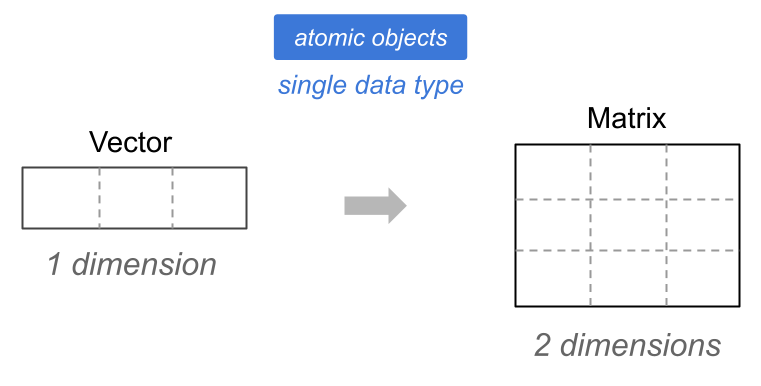
\includegraphics[width=0.6\linewidth]{images/objects/data-vector-matrix} \end{center}

\hypertarget{column-binding-vectors}{%
\subsubsection*{Column binding vectors}\label{column-binding-vectors}}
\addcontentsline{toc}{subsubsection}{Column binding vectors}

You can build a matrix by \textbf{column binding} vectors using the function
\texttt{cbind()}:

\begin{Shaded}
\begin{Highlighting}[]
\CommentTok{\# inputs}
\NormalTok{deposit }\OtherTok{=} \DecValTok{1000}
\NormalTok{rate }\OtherTok{=} \FloatTok{0.02}
\NormalTok{years }\OtherTok{=} \DecValTok{0}\SpecialCharTok{:}\DecValTok{5}

\CommentTok{\# future values}
\NormalTok{amounts }\OtherTok{=}\NormalTok{ deposit }\SpecialCharTok{*}\NormalTok{ (}\DecValTok{1} \SpecialCharTok{+}\NormalTok{ rate)}\SpecialCharTok{\^{}}\NormalTok{years}

\CommentTok{\# output as a matrix via cbind()}
\NormalTok{savings }\OtherTok{=} \FunctionTok{cbind}\NormalTok{(years, amounts)}
\NormalTok{savings}
\CommentTok{\#\textgreater{}      years  amounts}
\CommentTok{\#\textgreater{} [1,]     0 1000.000}
\CommentTok{\#\textgreater{} [2,]     1 1020.000}
\CommentTok{\#\textgreater{} [3,]     2 1040.400}
\CommentTok{\#\textgreater{} [4,]     3 1061.208}
\CommentTok{\#\textgreater{} [5,]     4 1082.432}
\CommentTok{\#\textgreater{} [6,]     5 1104.081}
\end{Highlighting}
\end{Shaded}

As you can tell, the use of \texttt{cbind()} is straightforward. All you have to do
is indicate the name of the vectors, separating them with a comma. Each vector
will become a column of the returned matrix.

\hypertarget{row-binding-vectors}{%
\subsubsection*{Row binding vectors}\label{row-binding-vectors}}
\addcontentsline{toc}{subsubsection}{Row binding vectors}

You can also build a matrix by \textbf{row binding} vectors.

\begin{Shaded}
\begin{Highlighting}[]
\NormalTok{savings }\OtherTok{=} \FunctionTok{rbind}\NormalTok{(years, amounts)}
\NormalTok{savings}
\CommentTok{\#\textgreater{}         [,1] [,2]   [,3]     [,4]     [,5]}
\CommentTok{\#\textgreater{} years      0    1    2.0    3.000    4.000}
\CommentTok{\#\textgreater{} amounts 1000 1020 1040.4 1061.208 1082.432}
\CommentTok{\#\textgreater{}             [,6]}
\CommentTok{\#\textgreater{} years      5.000}
\CommentTok{\#\textgreater{} amounts 1104.081}
\end{Highlighting}
\end{Shaded}

The difference between \texttt{cbind()} and \texttt{rbind()} is that the latter will ``stack''
the given vectors on top of each other. That is, each vector will become a row
of the returned matrix.

\hypertarget{creating-matrices-with-matrix}{%
\section{\texorpdfstring{Creating matrices with \texttt{matrix()}}{Creating matrices with matrix()}}\label{creating-matrices-with-matrix}}

More commonly, you use the function \texttt{matrix()} to create a matrix by providing
an input vector, and defining the number of rows and columns
(i.e.~the \emph{matrix dimensions}).

\begin{Shaded}
\begin{Highlighting}[]
\NormalTok{savings }\OtherTok{=} \FunctionTok{matrix}\NormalTok{(}\FunctionTok{c}\NormalTok{(years, amounts), }\AttributeTok{nrow =} \DecValTok{6}\NormalTok{, }\AttributeTok{ncol =} \DecValTok{2}\NormalTok{)}
\NormalTok{savings}
\CommentTok{\#\textgreater{}      [,1]     [,2]}
\CommentTok{\#\textgreater{} [1,]    0 1000.000}
\CommentTok{\#\textgreater{} [2,]    1 1020.000}
\CommentTok{\#\textgreater{} [3,]    2 1040.400}
\CommentTok{\#\textgreater{} [4,]    3 1061.208}
\CommentTok{\#\textgreater{} [5,]    4 1082.432}
\CommentTok{\#\textgreater{} [6,]    5 1104.081}
\end{Highlighting}
\end{Shaded}

The input vector \texttt{c(years,\ amounts)} is arranged into 6 rows and 2
columns.

\hypertarget{giving-names-to-rows-and-columns}{%
\subsubsection*{Giving names to rows and columns}\label{giving-names-to-rows-and-columns}}
\addcontentsline{toc}{subsubsection}{Giving names to rows and columns}

Often, you may need to provide names for either rows and columns

\begin{Shaded}
\begin{Highlighting}[]
\NormalTok{savings }\OtherTok{=} \FunctionTok{matrix}\NormalTok{(}\FunctionTok{c}\NormalTok{(years, amounts), }\AttributeTok{nrow =} \DecValTok{6}\NormalTok{, }\AttributeTok{ncol =} \DecValTok{2}\NormalTok{)}
\FunctionTok{rownames}\NormalTok{(savings) }\OtherTok{=} \DecValTok{1}\SpecialCharTok{:}\DecValTok{6}
\FunctionTok{colnames}\NormalTok{(savings) }\OtherTok{=} \FunctionTok{c}\NormalTok{(}\StringTok{"year"}\NormalTok{, }\StringTok{"amount"}\NormalTok{)}
\NormalTok{savings}
\CommentTok{\#\textgreater{}   year   amount}
\CommentTok{\#\textgreater{} 1    0 1000.000}
\CommentTok{\#\textgreater{} 2    1 1020.000}
\CommentTok{\#\textgreater{} 3    2 1040.400}
\CommentTok{\#\textgreater{} 4    3 1061.208}
\CommentTok{\#\textgreater{} 5    4 1082.432}
\CommentTok{\#\textgreater{} 6    5 1104.081}
\end{Highlighting}
\end{Shaded}

\hypertarget{more-matrices}{%
\subsection{More Matrices}\label{more-matrices}}

Let's make things a bit more complex. Say you have the following investments:

\begin{itemize}
\item
  \$1000 in a \textbf{savings account} that pays 2\% annual return, during 4 years
\item
  \$2000 in a \textbf{money market} account that pays 2.5\% annual return, during
  2 years
\item
  \$5000 in a \textbf{certificate of deposit} that pays 3\% annual return, during
  3 years
\end{itemize}

In R, we can calculate the future values of each type of investment product:

\begin{Shaded}
\begin{Highlighting}[]
\CommentTok{\# savings account}
\NormalTok{savings }\OtherTok{=} \DecValTok{1000} \SpecialCharTok{*}\NormalTok{ (}\DecValTok{1} \SpecialCharTok{+} \FloatTok{0.02}\NormalTok{)}\SpecialCharTok{\^{}}\NormalTok{(}\DecValTok{0}\SpecialCharTok{:}\DecValTok{4}\NormalTok{)}
\NormalTok{savings}
\CommentTok{\#\textgreater{} [1] 1000.000 1020.000 1040.400 1061.208 1082.432}
\end{Highlighting}
\end{Shaded}

\begin{Shaded}
\begin{Highlighting}[]
\CommentTok{\# money market}
\NormalTok{moneymkt }\OtherTok{=} \DecValTok{2000} \SpecialCharTok{*}\NormalTok{ (}\DecValTok{1} \SpecialCharTok{+} \FloatTok{0.025}\NormalTok{)}\SpecialCharTok{\^{}}\NormalTok{(}\DecValTok{0}\SpecialCharTok{:}\DecValTok{2}\NormalTok{)}
\NormalTok{moneymkt}
\CommentTok{\#\textgreater{} [1] 2000.00 2050.00 2101.25}
\end{Highlighting}
\end{Shaded}

\begin{Shaded}
\begin{Highlighting}[]
\CommentTok{\# certificate of deposit}
\NormalTok{certificate }\OtherTok{=} \DecValTok{5000} \SpecialCharTok{*}\NormalTok{ (}\DecValTok{1} \SpecialCharTok{+} \FloatTok{0.03}\NormalTok{)}\SpecialCharTok{\^{}}\NormalTok{(}\DecValTok{0}\SpecialCharTok{:}\DecValTok{3}\NormalTok{)}
\NormalTok{certificate}
\CommentTok{\#\textgreater{} [1] 5000.000 5150.000 5304.500 5463.635}
\end{Highlighting}
\end{Shaded}

\hypertarget{separated-matrices}{%
\subsubsection*{Separated matrices}\label{separated-matrices}}
\addcontentsline{toc}{subsubsection}{Separated matrices}

We can create individual matrices:

\begin{Shaded}
\begin{Highlighting}[]
\NormalTok{sav\_mat }\OtherTok{=} \FunctionTok{cbind}\NormalTok{(}\DecValTok{0}\SpecialCharTok{:}\DecValTok{4}\NormalTok{, savings)}

\NormalTok{mm\_mat }\OtherTok{=} \FunctionTok{cbind}\NormalTok{(}\DecValTok{0}\SpecialCharTok{:}\DecValTok{2}\NormalTok{, moneymkt)}

\NormalTok{cd\_mat }\OtherTok{=} \FunctionTok{cbind}\NormalTok{(}\DecValTok{0}\SpecialCharTok{:}\DecValTok{3}\NormalTok{, certificate)}
\end{Highlighting}
\end{Shaded}

Or we can stack everything into a single matrix:

\begin{Shaded}
\begin{Highlighting}[]
\FunctionTok{cbind}\NormalTok{(}\FunctionTok{c}\NormalTok{(}\DecValTok{0}\SpecialCharTok{:}\DecValTok{4}\NormalTok{, }\DecValTok{0}\SpecialCharTok{:}\DecValTok{2}\NormalTok{, }\DecValTok{0}\SpecialCharTok{:}\DecValTok{3}\NormalTok{), }\FunctionTok{c}\NormalTok{(savings, moneymkt, certificate))}
\CommentTok{\#\textgreater{}       [,1]     [,2]}
\CommentTok{\#\textgreater{}  [1,]    0 1000.000}
\CommentTok{\#\textgreater{}  [2,]    1 1020.000}
\CommentTok{\#\textgreater{}  [3,]    2 1040.400}
\CommentTok{\#\textgreater{}  [4,]    3 1061.208}
\CommentTok{\#\textgreater{}  [5,]    4 1082.432}
\CommentTok{\#\textgreater{}  [6,]    0 2000.000}
\CommentTok{\#\textgreater{}  [7,]    1 2050.000}
\CommentTok{\#\textgreater{}  [8,]    2 2101.250}
\CommentTok{\#\textgreater{}  [9,]    0 5000.000}
\CommentTok{\#\textgreater{} [10,]    1 5150.000}
\CommentTok{\#\textgreater{} [11,]    2 5304.500}
\CommentTok{\#\textgreater{} [12,]    3 5463.635}
\end{Highlighting}
\end{Shaded}

What if you want some table like this:

\begin{longtable}[]{@{}ccc@{}}
\toprule
account & year & amount \\
\midrule
\endhead
savings & 0 & 1000.000 \\
savings & 1 & 1020.000 \\
savings & 2 & 1040.400 \\
savings & 3 & 1061.208 \\
savings & 4 & 1082.432 \\
moneymkt & 0 & 2000.000 \\
moneymkt & 1 & 2050.000 \\
moneymkt & 2 & 2101.250 \\
certif & 0 & 5000.000 \\
certif & 1 & 5150.250 \\
certif & 2 & 5304.500 \\
certif & 3 & 5463.635 \\
\bottomrule
\end{longtable}

We could use the \texttt{cbind()} function in an attempt to obtain a matrix having
a similar rectangular structure as in the above table:

\begin{Shaded}
\begin{Highlighting}[]
\NormalTok{investments }\OtherTok{=} \FunctionTok{cbind}\NormalTok{(}
  \FunctionTok{rep}\NormalTok{(}\FunctionTok{c}\NormalTok{(}\StringTok{"savings"}\NormalTok{, }\StringTok{"moneymkt"}\NormalTok{, }\StringTok{"certif"}\NormalTok{), }\AttributeTok{times =} \FunctionTok{c}\NormalTok{(}\DecValTok{5}\NormalTok{, }\DecValTok{3}\NormalTok{, }\DecValTok{4}\NormalTok{)),}
  \FunctionTok{c}\NormalTok{(}\DecValTok{0}\SpecialCharTok{:}\DecValTok{4}\NormalTok{, }\DecValTok{0}\SpecialCharTok{:}\DecValTok{2}\NormalTok{, }\DecValTok{0}\SpecialCharTok{:}\DecValTok{3}\NormalTok{), }
  \FunctionTok{c}\NormalTok{(savings, moneymkt, certificate))}

\NormalTok{investments}
\CommentTok{\#\textgreater{}       [,1]       [,2] [,3]        }
\CommentTok{\#\textgreater{}  [1,] "savings"  "0"  "1000"      }
\CommentTok{\#\textgreater{}  [2,] "savings"  "1"  "1020"      }
\CommentTok{\#\textgreater{}  [3,] "savings"  "2"  "1040.4"    }
\CommentTok{\#\textgreater{}  [4,] "savings"  "3"  "1061.208"  }
\CommentTok{\#\textgreater{}  [5,] "savings"  "4"  "1082.43216"}
\CommentTok{\#\textgreater{}  [6,] "moneymkt" "0"  "2000"      }
\CommentTok{\#\textgreater{}  [7,] "moneymkt" "1"  "2050"      }
\CommentTok{\#\textgreater{}  [8,] "moneymkt" "2"  "2101.25"   }
\CommentTok{\#\textgreater{}  [9,] "certif"   "0"  "5000"      }
\CommentTok{\#\textgreater{} [10,] "certif"   "1"  "5150"      }
\CommentTok{\#\textgreater{} [11,] "certif"   "2"  "5304.5"    }
\CommentTok{\#\textgreater{} [12,] "certif"   "3"  "5463.635"}
\end{Highlighting}
\end{Shaded}

Do you notice something funny with the matrix \texttt{investments}?

As you can tell, all the values in \texttt{investments} are displayed being surrounded
with double quotes. This indicates that all the values are of type \texttt{character}.
Why?

Recall that matrices are \textbf{atomic} objects. Therefore, all the values in a
matrix must be of the same data type. In this example, because the first
input vector to \texttt{cbind()} is a character vector, which dominates other data
types, this will dictate the type of the produced matrix \texttt{investments}.

\hypertarget{lists}{%
\chapter{Lists}\label{lists}}

In this chapter, you will learn about R lists, the most generic type of data
container in R. Here's a summary of the main features of R lists:

\begin{itemize}
\tightlist
\item
  Lists are the most general class of data container
\item
  Like vectors, lists group data into a one-dimensional set
\item
  Unlike vectors, lists can store all kinds of objects
\item
  Lists can be of any length
\item
  Elements of a list can be named, or not
\end{itemize}

\hypertarget{creating-lists}{%
\section{Creating Lists}\label{creating-lists}}

The typical way to create a list is with the function \texttt{list()}. This function
creates a list the same way \texttt{c()} creates a vector. Let's start with a simple
example creating three numeric vectors of same length, that we then use to
store them in a list:

\begin{Shaded}
\begin{Highlighting}[]
\NormalTok{vec1 }\OtherTok{\textless{}{-}} \DecValTok{1}\SpecialCharTok{:}\DecValTok{3}
\NormalTok{vec2 }\OtherTok{\textless{}{-}} \DecValTok{4}\SpecialCharTok{:}\DecValTok{6}
\NormalTok{vec3 }\OtherTok{\textless{}{-}} \DecValTok{7}\SpecialCharTok{:}\DecValTok{9}

\CommentTok{\# list with unnamed elements}
\NormalTok{lis }\OtherTok{\textless{}{-}} \FunctionTok{list}\NormalTok{(vec1, vec2, vec3)}
\NormalTok{lis}
\CommentTok{\#\textgreater{} [[1]]}
\CommentTok{\#\textgreater{} [1] 1 2 3}
\CommentTok{\#\textgreater{} }
\CommentTok{\#\textgreater{} [[2]]}
\CommentTok{\#\textgreater{} [1] 4 5 6}
\CommentTok{\#\textgreater{} }
\CommentTok{\#\textgreater{} [[3]]}
\CommentTok{\#\textgreater{} [1] 7 8 9}
\end{Highlighting}
\end{Shaded}

Note how the contents of a list with unnamed elements are displayed: there is a
set of double brackets with an index indicating the position of each element,
and below each double bracket the corresponding vector is printed.

For illustration purposes, we could visualize the three input vectors and the
list with the following conceptual diagram.

\begin{figure}

{\centering 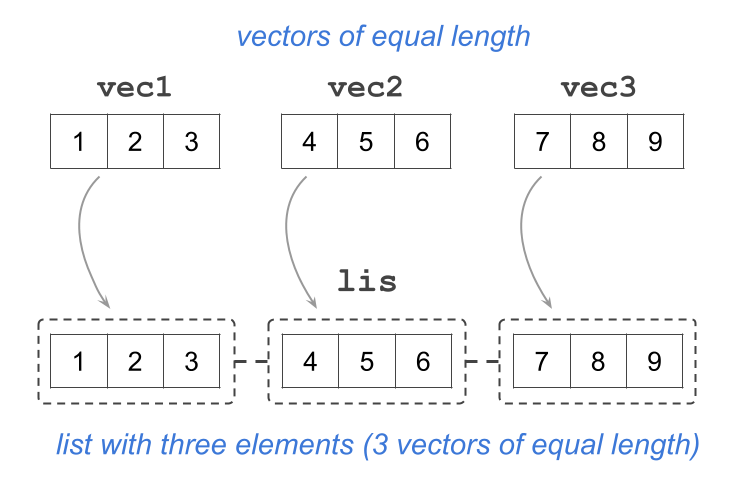
\includegraphics[width=0.6\linewidth]{images/objects/obj-list-vectors1} 

}

\caption{A list containing three unnamed elements (numeric vectors of length 3)}\label{fig:unnamed-chunk-112}
\end{figure}

Our intention with the depicted list as a set of discontinuous cells is to
convey the idea that a list is also a one-dimensional vector, albeit a very
special type of vector: a \textbf{non-atomic vector}. This means that each element
of a list can be any kind of object.

In the same way you can give names to elements of a vector, you can also give
names to elements of a list:

\begin{Shaded}
\begin{Highlighting}[]
\CommentTok{\# list with named elements}
\NormalTok{lis }\OtherTok{\textless{}{-}} \FunctionTok{list}\NormalTok{(}\StringTok{"vec1"} \OtherTok{=}\NormalTok{ vec1, }\StringTok{"vec2"} \OtherTok{=}\NormalTok{ vec2, }\StringTok{"vec3"} \OtherTok{=}\NormalTok{ vec3)}
\NormalTok{lis}
\CommentTok{\#\textgreater{} $vec1}
\CommentTok{\#\textgreater{} [1] 1 2 3}
\CommentTok{\#\textgreater{} }
\CommentTok{\#\textgreater{} $vec2}
\CommentTok{\#\textgreater{} [1] 4 5 6}
\CommentTok{\#\textgreater{} }
\CommentTok{\#\textgreater{} $vec3}
\CommentTok{\#\textgreater{} [1] 7 8 9}
\end{Highlighting}
\end{Shaded}

When you create a list in this form, you can actually omit the quotes of
the given names. While this option of naming elements may create a bit of
confusion for beginners and inexperienced users in R, we believe it's not a big
deal (based on our experience):

\begin{Shaded}
\begin{Highlighting}[]
\CommentTok{\# another option for giving names to elements in a list}
\NormalTok{lis }\OtherTok{\textless{}{-}} \FunctionTok{list}\NormalTok{(}\AttributeTok{vec1 =}\NormalTok{ vec1, }\AttributeTok{vec2 =}\NormalTok{ vec2, }\AttributeTok{vec3 =}\NormalTok{ vec3)}
\NormalTok{lis}
\CommentTok{\#\textgreater{} $vec1}
\CommentTok{\#\textgreater{} [1] 1 2 3}
\CommentTok{\#\textgreater{} }
\CommentTok{\#\textgreater{} $vec2}
\CommentTok{\#\textgreater{} [1] 4 5 6}
\CommentTok{\#\textgreater{} }
\CommentTok{\#\textgreater{} $vec3}
\CommentTok{\#\textgreater{} [1] 7 8 9}
\end{Highlighting}
\end{Shaded}

Observe how the contents of a list with named elements are displayed: this time,
instead of the set of double brackets, there is a dollar sign followed by the
name of the element, e.g.~\texttt{\$vec1}. Below each name, the corresponding vector is
printed.

The conceptual diagram in this case could look like this:

\begin{figure}

{\centering 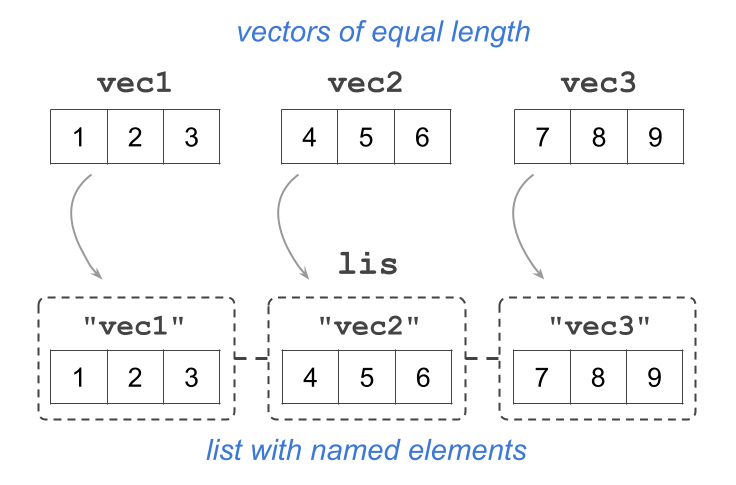
\includegraphics[width=0.6\linewidth]{images/objects/obj-list-vectors2} 

}

\caption{A list with named elements (numeric vectors of length 3)}\label{fig:unnamed-chunk-115}
\end{figure}

As we just said, the elements of a list can be any kind of R object. For
example, here's a list called \texttt{lst} that contains a character vector, a
numeric matrix, a factor, and another list:

\begin{Shaded}
\begin{Highlighting}[]
\NormalTok{lst }\OtherTok{\textless{}{-}} \FunctionTok{list}\NormalTok{(}
  \FunctionTok{c}\NormalTok{(}\StringTok{"Harry"}\NormalTok{, }\StringTok{"Ron"}\NormalTok{, }\StringTok{"Hermione"}\NormalTok{),}
  \FunctionTok{matrix}\NormalTok{(}\DecValTok{1}\SpecialCharTok{:}\DecValTok{6}\NormalTok{, }\AttributeTok{nrow =} \DecValTok{2}\NormalTok{, }\AttributeTok{ncol =} \DecValTok{3}\NormalTok{),}
  \FunctionTok{factor}\NormalTok{(}\FunctionTok{c}\NormalTok{(}\StringTok{"yes"}\NormalTok{, }\StringTok{"no"}\NormalTok{, }\StringTok{"no"}\NormalTok{, }\StringTok{"no"}\NormalTok{, }\StringTok{"yes"}\NormalTok{)),}
  \FunctionTok{list}\NormalTok{(}\StringTok{"Harry"}\NormalTok{, }\StringTok{"Ron"}\NormalTok{, }\StringTok{"Hermione"}\NormalTok{)}
\NormalTok{)}

\NormalTok{lst}
\CommentTok{\#\textgreater{} [[1]]}
\CommentTok{\#\textgreater{} [1] "Harry"    "Ron"      "Hermione"}
\CommentTok{\#\textgreater{} }
\CommentTok{\#\textgreater{} [[2]]}
\CommentTok{\#\textgreater{}      [,1] [,2] [,3]}
\CommentTok{\#\textgreater{} [1,]    1    3    5}
\CommentTok{\#\textgreater{} [2,]    2    4    6}
\CommentTok{\#\textgreater{} }
\CommentTok{\#\textgreater{} [[3]]}
\CommentTok{\#\textgreater{} [1] yes no  no  no  yes}
\CommentTok{\#\textgreater{} Levels: no yes}
\CommentTok{\#\textgreater{} }
\CommentTok{\#\textgreater{} [[4]]}
\CommentTok{\#\textgreater{} [[4]][[1]]}
\CommentTok{\#\textgreater{} [1] "Harry"}
\CommentTok{\#\textgreater{} }
\CommentTok{\#\textgreater{} [[4]][[2]]}
\CommentTok{\#\textgreater{} [1] "Ron"}
\CommentTok{\#\textgreater{} }
\CommentTok{\#\textgreater{} [[4]][[3]]}
\CommentTok{\#\textgreater{} [1] "Hermione"}
\end{Highlighting}
\end{Shaded}

Whenever possible, we strongly recommend giving names to the elements of a list.
Not only this makes it easy to identify one element from the others, but it also
gives you more flexibility to rearrange the contents of the list without having
to worry about the exact order or position they occupy.

\begin{Shaded}
\begin{Highlighting}[]
\CommentTok{\# whenever possible, give names to elements in a list}
\NormalTok{lst }\OtherTok{\textless{}{-}} \FunctionTok{list}\NormalTok{(}
  \AttributeTok{first =} \FunctionTok{c}\NormalTok{(}\StringTok{"Harry"}\NormalTok{, }\StringTok{"Ron"}\NormalTok{, }\StringTok{"Hermione"}\NormalTok{),}
  \AttributeTok{second =} \FunctionTok{matrix}\NormalTok{(}\DecValTok{1}\SpecialCharTok{:}\DecValTok{6}\NormalTok{, }\AttributeTok{nrow =} \DecValTok{2}\NormalTok{, }\AttributeTok{ncol =} \DecValTok{3}\NormalTok{),}
  \AttributeTok{third =} \FunctionTok{factor}\NormalTok{(}\FunctionTok{c}\NormalTok{(}\StringTok{"yes"}\NormalTok{, }\StringTok{"no"}\NormalTok{, }\StringTok{"no"}\NormalTok{, }\StringTok{"no"}\NormalTok{, }\StringTok{"yes"}\NormalTok{)),}
  \AttributeTok{fourth =} \FunctionTok{list}\NormalTok{(}\StringTok{"Harry"}\NormalTok{, }\StringTok{"Ron"}\NormalTok{, }\StringTok{"Hermione"}\NormalTok{)}
\NormalTok{)}
\end{Highlighting}
\end{Shaded}

\hypertarget{manipulating-lists}{%
\section{Manipulating Lists}\label{manipulating-lists}}

To manipulate the elements of a list you can use bracket notation. Because a
list is a vector, you can use single brackets (e.g.~\texttt{lis{[}1{]}}) as well as
double brackets (e.g.~\texttt{lis{[}{[}1{]}{]}}).

\begin{figure}

{\centering 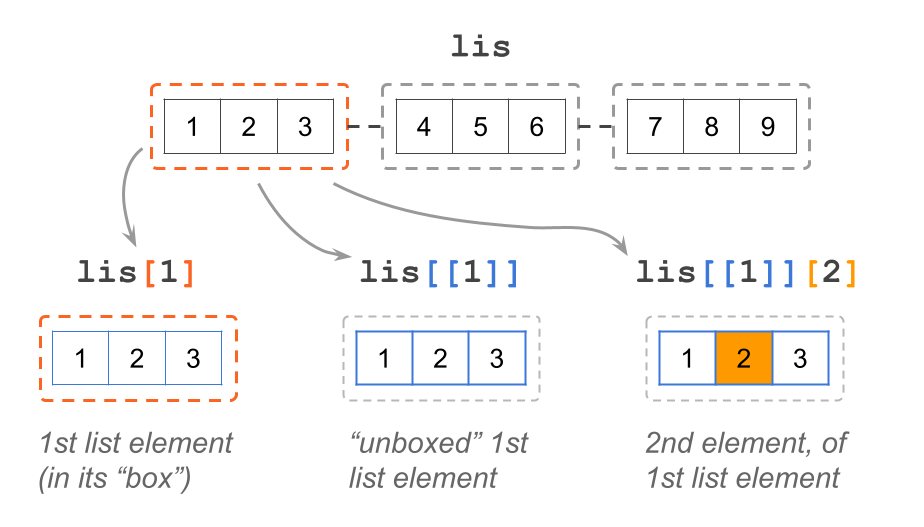
\includegraphics[width=0.75\linewidth]{images/objects/obj-list-brackets1} 

}

\caption{Bracket notation with lists}\label{fig:unnamed-chunk-118}
\end{figure}

\hypertarget{single-brackets}{%
\subsection{Single brackets}\label{single-brackets}}

Just like any other vector, and any other data object in R, you can use single
brackets on a list. For example, consider the unnamed version of a list, and
the use of single brackets with index \texttt{1} inside them:

\begin{Shaded}
\begin{Highlighting}[]
\CommentTok{\# list with unnamed elements}
\NormalTok{lis }\OtherTok{\textless{}{-}} \FunctionTok{list}\NormalTok{(vec1, vec2, vec3)}

\NormalTok{lis[}\DecValTok{1}\NormalTok{]}
\CommentTok{\#\textgreater{} [[1]]}
\CommentTok{\#\textgreater{} [1] 1 2 3}
\end{Highlighting}
\end{Shaded}

What a single bracket does, is give you access to the ``container'' of the
specified element but without ``unboxing'' its contents. This is reflected by
the way in which the output is displayed: note the double bracket \texttt{{[}{[}1{]}{]}} in
the first line, and then \texttt{{[}1{]}\ 1\ 2\ 3} in the second line.

In other words, \texttt{lis{[}1{]}} gives you the first element of the list, which
contains a vector, but it does not give you direct access to the vector itself.
Put another way, \texttt{lis{[}1{]}} lets you see that the first element of the list is
a vector, but this vector is still \emph{inside} its ``box''.

\begin{figure}

{\centering 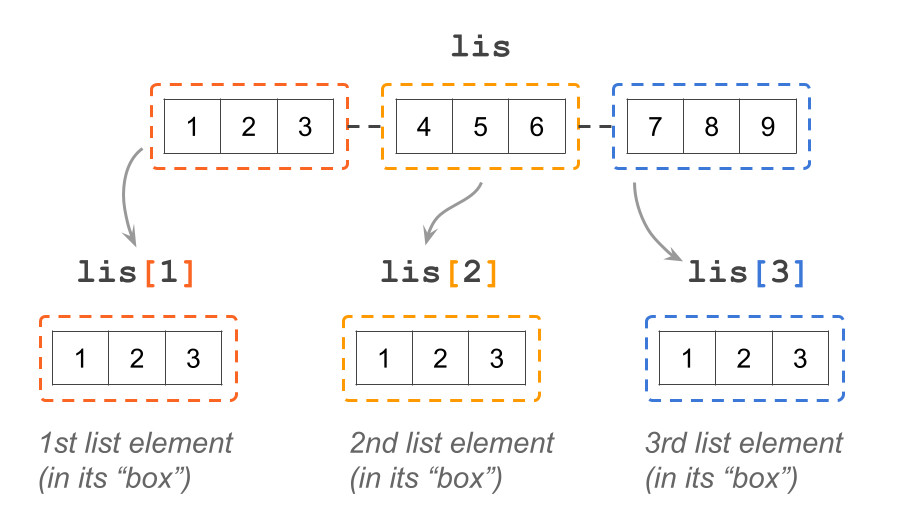
\includegraphics[width=0.75\linewidth]{images/objects/obj-list-brackets2} 

}

\caption{Use single brackets to select an element}\label{fig:unnamed-chunk-120}
\end{figure}

\hypertarget{double-brackets}{%
\subsection{Double Brackets}\label{double-brackets}}

In addition to single brackets, lists also accept double brackets: e.g.~
\texttt{lis{[}{[}1{]}{]}}

\begin{Shaded}
\begin{Highlighting}[]
\NormalTok{lis[[}\DecValTok{1}\NormalTok{]]}
\CommentTok{\#\textgreater{} [1] 1 2 3}
\end{Highlighting}
\end{Shaded}

Double brackets are used when you want to get access to the content of the
list's elements. Notice the output of the previous command: now there are no
double brackets, just the output of the vector in the first position. Think
of this command as ``unboxing'' the object of the first element in \texttt{lis}.

What if you want to manipulate the elements of vector \texttt{vec1} or \texttt{vec2}? Use
double brackets followed by single brackets

\begin{Shaded}
\begin{Highlighting}[]
\CommentTok{\# second index of first list\textquotesingle{}s element}
\NormalTok{lis[[}\DecValTok{1}\NormalTok{]][}\DecValTok{2}\NormalTok{]}
\CommentTok{\#\textgreater{} [1] 2}

\CommentTok{\# first index of second list\textquotesingle{}s element}
\NormalTok{lis[[}\DecValTok{2}\NormalTok{]][}\DecValTok{1}\NormalTok{]}
\CommentTok{\#\textgreater{} [1] 4}
\end{Highlighting}
\end{Shaded}

\begin{figure}

{\centering 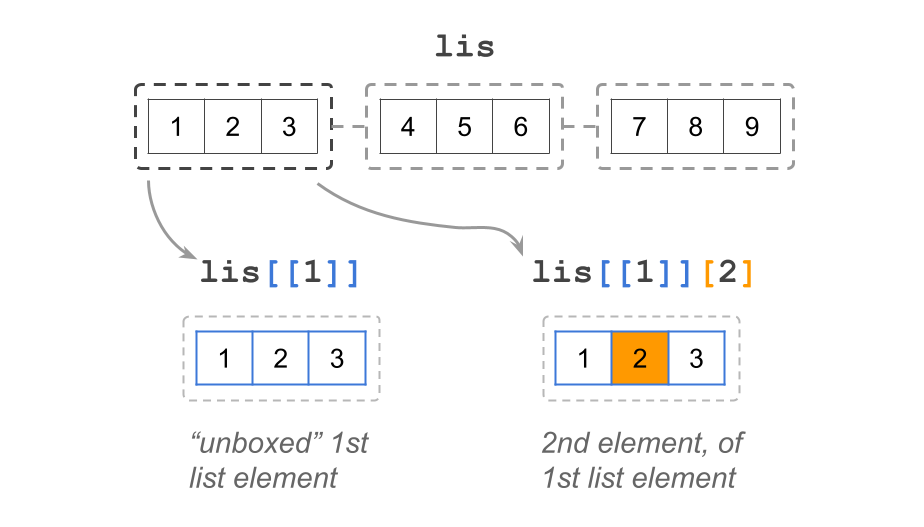
\includegraphics[width=0.75\linewidth]{images/objects/obj-list-brackets3} 

}

\caption{Use double brackets to extract an element}\label{fig:unnamed-chunk-123}
\end{figure}

\hypertarget{dollar-signs}{%
\subsection{Dollar signs}\label{dollar-signs}}

R lists---and data frames---follow an optional second system of notation for
extracting \textbf{named elements} using the dollar sign \textbf{\texttt{\$}}

\begin{figure}

{\centering 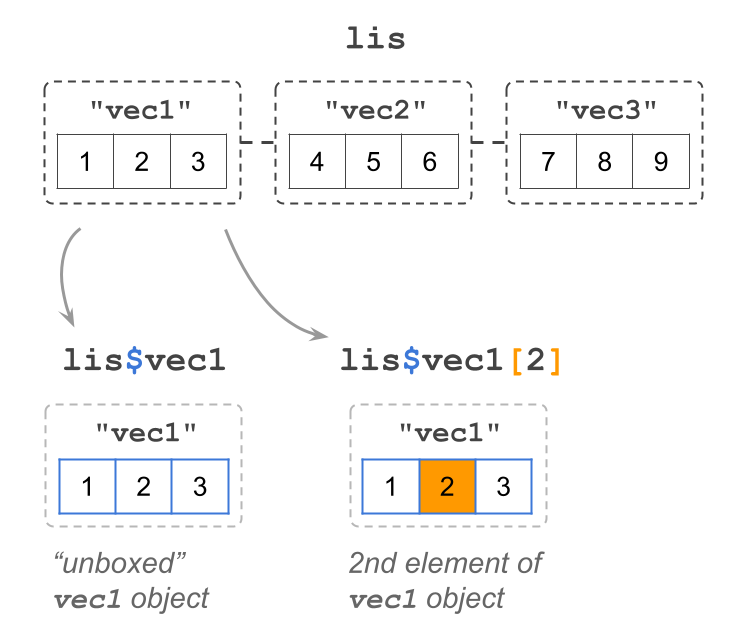
\includegraphics[width=0.6\linewidth]{images/objects/obj-list-dollars1} 

}

\caption{Dollar notation with lists}\label{fig:unnamed-chunk-124}
\end{figure}

Let's use the named version of \texttt{lis}:

\begin{Shaded}
\begin{Highlighting}[]
\CommentTok{\# list with named elements}
\NormalTok{lis }\OtherTok{\textless{}{-}} \FunctionTok{list}\NormalTok{(}\StringTok{"vec1"} \OtherTok{=}\NormalTok{ vec1, }\StringTok{"vec2"} \OtherTok{=}\NormalTok{ vec2, }\StringTok{"vec3"} \OtherTok{=}\NormalTok{ vec3)}

\NormalTok{lis}\SpecialCharTok{$}\NormalTok{vec1}
\CommentTok{\#\textgreater{} [1] 1 2 3}
\end{Highlighting}
\end{Shaded}

The dollar sign \textbf{\texttt{\$}} notation works for selecting \textbf{named elements} in a
list. Notice the output of the above command: \texttt{lis\$vec1} gives you vector
\texttt{1\ 2\ 3}. In other words, dollar notation ``unboxes'' the object that is associated
to the specified name.

\hypertarget{adding-new-elements}{%
\subsection{Adding new elements}\label{adding-new-elements}}

From time to time, you will want to add one or more elements to an existing
list. For instance, consider a list \texttt{lst} with two elements:

\begin{Shaded}
\begin{Highlighting}[]
\NormalTok{lst }\OtherTok{\textless{}{-}} \FunctionTok{list}\NormalTok{(}\DecValTok{1}\SpecialCharTok{:}\DecValTok{3}\NormalTok{, }\FunctionTok{c}\NormalTok{(}\StringTok{\textquotesingle{}A\textquotesingle{}}\NormalTok{, }\StringTok{\textquotesingle{}B\textquotesingle{}}\NormalTok{, }\StringTok{\textquotesingle{}C\textquotesingle{}}\NormalTok{))}

\NormalTok{lst}
\CommentTok{\#\textgreater{} [[1]]}
\CommentTok{\#\textgreater{} [1] 1 2 3}
\CommentTok{\#\textgreater{} }
\CommentTok{\#\textgreater{} [[2]]}
\CommentTok{\#\textgreater{} [1] "A" "B" "C"}
\end{Highlighting}
\end{Shaded}

Say you want to add a logical vector as a third element to \texttt{lst}. One option to
do this is with double brackets, specifying a new index position to which you
assign the new element:

\begin{Shaded}
\begin{Highlighting}[]
\NormalTok{lst[[}\DecValTok{3}\NormalTok{]] }\OtherTok{\textless{}{-}} \FunctionTok{c}\NormalTok{(}\ConstantTok{TRUE}\NormalTok{, }\ConstantTok{FALSE}\NormalTok{, }\ConstantTok{TRUE}\NormalTok{, }\ConstantTok{FALSE}\NormalTok{)}

\NormalTok{lst}
\CommentTok{\#\textgreater{} [[1]]}
\CommentTok{\#\textgreater{} [1] 1 2 3}
\CommentTok{\#\textgreater{} }
\CommentTok{\#\textgreater{} [[2]]}
\CommentTok{\#\textgreater{} [1] "A" "B" "C"}
\CommentTok{\#\textgreater{} }
\CommentTok{\#\textgreater{} [[3]]}
\CommentTok{\#\textgreater{} [1]  TRUE FALSE  TRUE FALSE}
\end{Highlighting}
\end{Shaded}

Another option is to use the dollar operator by giving a new name to which you
assign the new element. Even though the previous elements in \texttt{lst}are unnamed,
the new added element will have an associated label:

\begin{Shaded}
\begin{Highlighting}[]
\NormalTok{lst}\SpecialCharTok{$}\NormalTok{new\_elem }\OtherTok{\textless{}{-}} \StringTok{\textquotesingle{}nuevo\textquotesingle{}}

\NormalTok{lst}
\CommentTok{\#\textgreater{} [[1]]}
\CommentTok{\#\textgreater{} [1] 1 2 3}
\CommentTok{\#\textgreater{} }
\CommentTok{\#\textgreater{} [[2]]}
\CommentTok{\#\textgreater{} [1] "A" "B" "C"}
\CommentTok{\#\textgreater{} }
\CommentTok{\#\textgreater{} [[3]]}
\CommentTok{\#\textgreater{} [1]  TRUE FALSE  TRUE FALSE}
\CommentTok{\#\textgreater{} }
\CommentTok{\#\textgreater{} $new\_elem}
\CommentTok{\#\textgreater{} [1] "nuevo"}
\end{Highlighting}
\end{Shaded}

\hypertarget{removing-elements}{%
\subsection{Removing elements}\label{removing-elements}}

Just like you will want to add new elements in a list, you will also find
occasions in which you need to remove one or more elements. Take the previous
list \texttt{lst} with four elements, and say you want to remove the third element
(containing the logical vector)

\begin{Shaded}
\begin{Highlighting}[]
\NormalTok{lst}
\CommentTok{\#\textgreater{} [[1]]}
\CommentTok{\#\textgreater{} [1] 1 2 3}
\CommentTok{\#\textgreater{} }
\CommentTok{\#\textgreater{} [[2]]}
\CommentTok{\#\textgreater{} [1] "A" "B" "C"}
\CommentTok{\#\textgreater{} }
\CommentTok{\#\textgreater{} [[3]]}
\CommentTok{\#\textgreater{} [1]  TRUE FALSE  TRUE FALSE}
\CommentTok{\#\textgreater{} }
\CommentTok{\#\textgreater{} $new\_elem}
\CommentTok{\#\textgreater{} [1] "nuevo"}
\end{Highlighting}
\end{Shaded}

To remove the third element, which is unnamed, you use double brackets and
assign a value \texttt{NULL} to that position:

\begin{Shaded}
\begin{Highlighting}[]
\NormalTok{lst[[}\DecValTok{3}\NormalTok{]] }\OtherTok{\textless{}{-}} \ConstantTok{NULL}
\NormalTok{lst}
\CommentTok{\#\textgreater{} [[1]]}
\CommentTok{\#\textgreater{} [1] 1 2 3}
\CommentTok{\#\textgreater{} }
\CommentTok{\#\textgreater{} [[2]]}
\CommentTok{\#\textgreater{} [1] "A" "B" "C"}
\CommentTok{\#\textgreater{} }
\CommentTok{\#\textgreater{} $new\_elem}
\CommentTok{\#\textgreater{} [1] "nuevo"}
\end{Highlighting}
\end{Shaded}

As for those named elements, such as \texttt{lst\$new\_elem}, you do the same and assign
a \texttt{NULL} value, but this time using dollar notation:

\begin{Shaded}
\begin{Highlighting}[]
\NormalTok{lst}\SpecialCharTok{$}\NormalTok{new\_elem }\OtherTok{\textless{}{-}} \ConstantTok{NULL}
\NormalTok{lst}
\CommentTok{\#\textgreater{} [[1]]}
\CommentTok{\#\textgreater{} [1] 1 2 3}
\CommentTok{\#\textgreater{} }
\CommentTok{\#\textgreater{} [[2]]}
\CommentTok{\#\textgreater{} [1] "A" "B" "C"}
\end{Highlighting}
\end{Shaded}

\hypertarget{exercises-2}{%
\section{Exercises}\label{exercises-2}}

\textbf{1)} How would you create a list with your first name, middle name, and last
name? For example, something like:

\begin{verbatim}
$first
[1] "Gaston"

$middle
NULL

$last
[1] "Sanchez"
\end{verbatim}

\textbf{2)} Consider an R list \texttt{student} containing the following elements:

\begin{verbatim}
$name
[1] "Luke Skywalker"

$major_minor
              major               minor 
     "jedi studies" "imperial policies" 

$gpa
[1] 4

$grades
           course score
1       force-101   9.3
2    light-sabers  10.0
3 jedi-literature   8.5
\end{verbatim}

What is the output of the following commands? Try to guess the answer without
running the code.

\begin{enumerate}
\def\labelenumi{\alph{enumi})}
\item
  \texttt{student\$grades\$semester\ \textless{}-\ 4}
\item
  \texttt{sum(student{[}{[}2{]}{]}\ ==\ "sith\ philosophy")}
\item
  \texttt{student{[}"sid"{]}\ \textless{}-\ as.integer("123456")}
\item
  \texttt{mean(student{[}{[}4{]}{]}{[}1:3,2{]},\ na.rm\ =\ TRUE)}
\item
  \texttt{student{[}{[}4{]}{]}\ \textless{}-\ student\$grades{[}c(FALSE,\ TRUE,\ TRUE),\ {]}}
\end{enumerate}

\hypertarget{part-programming-basics}{%
\part{Programming Basics}\label{part-programming-basics}}

\hypertarget{functions1}{%
\chapter{Intro to Functions}\label{functions1}}

R comes with many functions and packages that let us perform a wide variety
of tasks, and so far we've been using a number of them. In fact, most of the
things we do in R is by calling some function. Sometimes, however, there is no
function to do what we want to achieve. When this is the case, we may very
well want to write our own functions.

In this chapter we'll describe how to start writing small and simple functions.
We are going to start covering the ``tip of the iceberg'', and in the following
chapters we will continue discussing more aspects about writing functions, and
describing how R works when you invoke (call) a function.

\hypertarget{motivation-1}{%
\section{Motivation}\label{motivation-1}}

We've used the formula of \textbf{future value}, given below, which is useful to
answer questions like: If you deposit \$1000 into a savings account that pays
an annual interest of 2\%, how much will you have at the end of year 10?

\[
\text{FV} = \text{PV} \times (1 + r)^t
\]

\begin{itemize}
\tightlist
\item
  \(\text{FV}\) = future value (how much you'll have)
\item
  \(\text{PV}\) = present value (the initial deposit)
\item
  \(r\) = rate of return (e.g.~annual rate of return)
\item
  \(t\) = number of periods (e.g.~number of years)
\end{itemize}

R has a large number of functions---e.g.~\texttt{sqrt()}, \texttt{log()}, \texttt{mean()},
\texttt{sd()}, \texttt{exp()}, etc---but it does not have a built-in function to compute
future value.

Wouldn't it be nice to have a \texttt{future\_value()} function---or an \texttt{fv()}
function---that you could call in R? Perhaps something like:

\begin{Shaded}
\begin{Highlighting}[]
\FunctionTok{future\_value}\NormalTok{(}\AttributeTok{present =} \DecValTok{1000}\NormalTok{, }\AttributeTok{rate =} \FloatTok{0.02}\NormalTok{, }\AttributeTok{year =} \DecValTok{10}\NormalTok{)}
\end{Highlighting}
\end{Shaded}

Let's create such a function!

\hypertarget{writing-a-simple-function}{%
\section{Writing a Simple Function}\label{writing-a-simple-function}}

This won't always be the case, but in our current example we have a specific
mathematical formula to work with (which makes things a lot easier):

\[
\text{FV} = \text{PV} \times (1 + r)^t
\]

Like other programming languages that can be used for scientific computations,
we can take advantage of the syntax in R to write an expression that is almost
identical to the algebraic formulation:

\begin{Shaded}
\begin{Highlighting}[]
\NormalTok{fv }\OtherTok{=}\NormalTok{ pv }\SpecialCharTok{*}\NormalTok{ (}\DecValTok{1} \SpecialCharTok{+}\NormalTok{ r)}\SpecialCharTok{\^{}}\NormalTok{t}
\end{Highlighting}
\end{Shaded}

We will use this simple line of code as our starting point for creating a
future value function. Here is how to do it ``logically'' step by step.

\hypertarget{step-1-start-with-a-concrete-example}{%
\subsubsection*{Step 1: Start with a concrete example}\label{step-1-start-with-a-concrete-example}}
\addcontentsline{toc}{subsubsection}{Step 1: Start with a concrete example}

You should always start with a \textbf{small and concrete example}, focusing
on writing code that does the job. For example, we could write the following
lines:

\begin{Shaded}
\begin{Highlighting}[]
\CommentTok{\# inputs}
\NormalTok{pv }\OtherTok{=} \DecValTok{1000}
\NormalTok{r }\OtherTok{=} \FloatTok{0.02}
\NormalTok{t }\OtherTok{=} \DecValTok{10}

\CommentTok{\# process}
\NormalTok{fv }\OtherTok{=}\NormalTok{ pv }\SpecialCharTok{*}\NormalTok{ (}\DecValTok{1} \SpecialCharTok{+}\NormalTok{ r)}\SpecialCharTok{\^{}}\NormalTok{t}

\CommentTok{\# output}
\NormalTok{fv}
\CommentTok{\#\textgreater{} [1] 1218.994}
\end{Highlighting}
\end{Shaded}

When I say ``small example'' I mean working with objects containing just a few
values. Here, the objects \texttt{pv}, \texttt{r}, and \texttt{t} are super simple vectors of size 1.
Sometimes, though, you may want to start with less simple---yet small---objects
containing just a couple of values. That's fine too.

Sometimes you may even need to start not just with one, but with a couple of
concrete examples that will help you get a better feeling of what kind of
objects, and operations you need to use.

As you get more experience creating and writing functions, you may want to
start with a ``medium-size'' concrete example. Personally, I don't tend to start
like this. Instead, I like to take baby-steps, and I also like to take my time,
without rushing the coding. You know the old-saying: ``measure twice, cut once.''

An important part of starting with a concrete example is so that you can
identify what the inputs are, what computations or process the inputs will go through, and what the output should be.

Inputs:

\begin{itemize}
\tightlist
\item
  \texttt{pv}
\item
  \texttt{r}
\item
  \texttt{t}
\end{itemize}

Process:

\begin{itemize}
\tightlist
\item
  \texttt{fv\ =\ pv\ *\ (1\ +\ r)\^{}t}
\end{itemize}

Output:

\begin{itemize}
\tightlist
\item
  \texttt{fv}
\end{itemize}

\hypertarget{step-2-make-your-code-more-generalizable}{%
\subsubsection*{Step 2: Make your code more generalizable}\label{step-2-make-your-code-more-generalizable}}
\addcontentsline{toc}{subsubsection}{Step 2: Make your code more generalizable}

After having one (or a few) concrete example(s), the next step is to make your
code more generalizable, or if you prefer, to make it more abstract (or at
least less concrete).

Instead of working with specific values \texttt{pv}, \texttt{r}, and \texttt{t}, you can give them
a more algebraic spirit. For instance, the code below considers ``open-ended''
inputs without assigning them any values

\begin{Shaded}
\begin{Highlighting}[]
\CommentTok{\# general inputs (could take "any" values)}
\NormalTok{pv}
\NormalTok{r}
\NormalTok{t}

\CommentTok{\# process}
\NormalTok{fv }\OtherTok{=}\NormalTok{ pv }\SpecialCharTok{*}\NormalTok{ (}\DecValTok{1} \SpecialCharTok{+}\NormalTok{ r)}\SpecialCharTok{\^{}}\NormalTok{t}

\CommentTok{\# output}
\NormalTok{fv}
\end{Highlighting}
\end{Shaded}

Obviously this piece of code is very abstract and not intended to be executed
in R; this is just for the sake of conceptual illustration.

\hypertarget{step-3-encapsulate-the-code-into-a-function}{%
\subsubsection*{Step 3: Encapsulate the code into a function}\label{step-3-encapsulate-the-code-into-a-function}}
\addcontentsline{toc}{subsubsection}{Step 3: Encapsulate the code into a function}

The next step is to encapsulate your code as a formal function in R. I will
show you how to do this in two logical substeps, although keep in mind that in
practice you will merge these two substeps into a single one.

The encapsulation process involves placing the ``inputs'' inside the function
\texttt{function()}, separating each input with a comma. Formally speaking, the
inputs of your functions are known as the \textbf{arguments} of the function.

Likewise, the lines of code that correspond to the ``process'' and ``output'' are
what will become the \textbf{body} of the function. Typically, you encapsulate the
code of the body by surrounding it with curly braces \texttt{\{\ \}}

\begin{Shaded}
\begin{Highlighting}[]
\CommentTok{\# encapsulating code into a function}
\ControlFlowTok{function}\NormalTok{(pv, r, t) \{}
\NormalTok{  fv }\OtherTok{=}\NormalTok{ pv }\SpecialCharTok{*}\NormalTok{ (}\DecValTok{1} \SpecialCharTok{+}\NormalTok{ r)}\SpecialCharTok{\^{}}\NormalTok{t}
\NormalTok{  fv}
\NormalTok{\}}
\end{Highlighting}
\end{Shaded}

The other substep typically consists of \textbf{assigning a name} to the code of
your function. For example, you can give it the name \texttt{FV}:

\begin{Shaded}
\begin{Highlighting}[]
\CommentTok{\# future value function}
\NormalTok{FV }\OtherTok{=} \ControlFlowTok{function}\NormalTok{(pv, r, t) \{}
\NormalTok{  fv }\OtherTok{=}\NormalTok{ pv }\SpecialCharTok{*}\NormalTok{ (}\DecValTok{1} \SpecialCharTok{+}\NormalTok{ r)}\SpecialCharTok{\^{}}\NormalTok{t}
\NormalTok{  fv}
\NormalTok{\}}
\end{Highlighting}
\end{Shaded}

In summary:

\begin{itemize}
\item
  the inputs go inside \texttt{function()}, separating each input with a comma
\item
  the processing step and the output are surrounded within curly braces \texttt{\{\ \}}
\item
  you typically assign a name to the code of your function
\end{itemize}

\hypertarget{step-4-test-that-the-function-works}{%
\subsubsection*{Step 4: Test that the function works}\label{step-4-test-that-the-function-works}}
\addcontentsline{toc}{subsubsection}{Step 4: Test that the function works}

Once the function is created, you test it to make sure that everything works.
Very likely you will test your function with the small and concrete example:

\begin{Shaded}
\begin{Highlighting}[]
\CommentTok{\# test it}
\FunctionTok{FV}\NormalTok{(}\DecValTok{1000}\NormalTok{, }\FloatTok{0.02}\NormalTok{, }\DecValTok{10}\NormalTok{)}
\CommentTok{\#\textgreater{} [1] 1218.994}
\end{Highlighting}
\end{Shaded}

And then you'll keep testing your function with other less simple examples.
In this case, because the code we are working with is based on vectors,
and uses common functions for vectors, we can further inspect the behavior of
the function by providing vectors of various sizes for all the arguments:

\begin{Shaded}
\begin{Highlighting}[]
\CommentTok{\# vectorized years}
\FunctionTok{FV}\NormalTok{(}\DecValTok{1000}\NormalTok{, }\FloatTok{0.02}\NormalTok{, }\DecValTok{1}\SpecialCharTok{:}\DecValTok{5}\NormalTok{)}
\CommentTok{\#\textgreater{} [1] 1020.000 1040.400 1061.208 1082.432 1104.081}
\end{Highlighting}
\end{Shaded}

\begin{Shaded}
\begin{Highlighting}[]
\CommentTok{\# vectorized rates}
\FunctionTok{FV}\NormalTok{(}\DecValTok{1000}\NormalTok{, }\FunctionTok{seq}\NormalTok{(}\FloatTok{0.01}\NormalTok{, }\FloatTok{0.02}\NormalTok{, }\AttributeTok{by =} \FloatTok{0.005}\NormalTok{), }\DecValTok{1}\NormalTok{)}
\CommentTok{\#\textgreater{} [1] 1010 1015 1020}
\end{Highlighting}
\end{Shaded}

\begin{Shaded}
\begin{Highlighting}[]
\CommentTok{\# vectorized present values}
\FunctionTok{FV}\NormalTok{(}\FunctionTok{c}\NormalTok{(}\DecValTok{1000}\NormalTok{, }\DecValTok{2000}\NormalTok{, }\DecValTok{3000}\NormalTok{), }\FloatTok{0.02}\NormalTok{, }\DecValTok{1}\NormalTok{)}
\CommentTok{\#\textgreater{} [1] 1020 2040 3060}
\end{Highlighting}
\end{Shaded}

Notice that the function is vectorized, this is because we are using arithmetic
operators (e.g.~multiplication, subtraction, division) which are in turn
vectorized.

\hypertarget{in-summary}{%
\subsubsection*{In Summary}\label{in-summary}}
\addcontentsline{toc}{subsubsection}{In Summary}

\begin{itemize}
\item
  To define a new function in R you use the function \texttt{function()}.
\item
  Usually, you specify a name for the function, and then assign \texttt{function()}
  to the chosen name.
\item
  You also need to define optional arguments (i.e.~inputs of the function).
\item
  And of course, you must write the code (i.e.~the body) so the function does
  something when you use it.
\end{itemize}

\hypertarget{arguments-with-default-values}{%
\subsection{Arguments with default values}\label{arguments-with-default-values}}

Sometimes it's a good idea to add a default value to one (or more) of the
arguments. For example, we could give default values to the arguments in such
a way that when the user executes the function without any input, \texttt{FV()}
returns the value of 100 monetary units invested at a rate of return of
1\% for 1 year:

\begin{Shaded}
\begin{Highlighting}[]
\CommentTok{\# future value function with default arguments}
\NormalTok{FV }\OtherTok{=} \ControlFlowTok{function}\NormalTok{(}\AttributeTok{pv =} \DecValTok{100}\NormalTok{, }\AttributeTok{r =} \FloatTok{0.01}\NormalTok{, }\AttributeTok{t =} \DecValTok{1}\NormalTok{) \{}
\NormalTok{  fv }\OtherTok{=}\NormalTok{ pv }\SpecialCharTok{*}\NormalTok{ (}\DecValTok{1} \SpecialCharTok{+}\NormalTok{ r)}\SpecialCharTok{\^{}}\NormalTok{t}
\NormalTok{  fv}
\NormalTok{\}}

\CommentTok{\# default execution}
\FunctionTok{FV}\NormalTok{()}
\CommentTok{\#\textgreater{} [1] 101}
\end{Highlighting}
\end{Shaded}

An interesting side effect of giving default values to the arguments of
a function is that you can also call it by specifying arguments in an order
different from the order in which the function was created:

\begin{Shaded}
\begin{Highlighting}[]
\FunctionTok{FV}\NormalTok{(}\AttributeTok{r =} \FloatTok{0.02}\NormalTok{, }\AttributeTok{t =} \DecValTok{3}\NormalTok{, }\AttributeTok{pv =} \DecValTok{1000}\NormalTok{)}
\CommentTok{\#\textgreater{} [1] 1061.208}
\end{Highlighting}
\end{Shaded}

\hypertarget{writing-functions-for-humans}{%
\section{Writing Functions for Humans}\label{writing-functions-for-humans}}

When writing functions (or coding in general), you should write code not just
for the computer, \textbf{but also for humans}. While it is true that R doesn't
care too much about what names and symbols you use, your code will be used by
a human being: either you or someone else. Which means that a human will have
to take a look at the code.

Here are some options to make our code more human friendly. We can give the
function a more descriptive name such as \texttt{future\_value()}. Likewise, we can
use more descriptive names for the arguments: e.g.~\texttt{present}, \texttt{rate}, and
\texttt{years}.

\begin{Shaded}
\begin{Highlighting}[]
\CommentTok{\# future value function}
\NormalTok{future\_value }\OtherTok{=} \ControlFlowTok{function}\NormalTok{(present, rate, years) \{}
\NormalTok{  future }\OtherTok{=}\NormalTok{ present }\SpecialCharTok{*}\NormalTok{ (}\DecValTok{1} \SpecialCharTok{+}\NormalTok{ rate)}\SpecialCharTok{\^{}}\NormalTok{years}
\NormalTok{  future}
\NormalTok{\}}

\CommentTok{\# test it}
\FunctionTok{future\_value}\NormalTok{(}\AttributeTok{present =} \DecValTok{1000}\NormalTok{, }\AttributeTok{rate =} \FloatTok{0.02}\NormalTok{, }\AttributeTok{years =} \DecValTok{10}\NormalTok{)}
\CommentTok{\#\textgreater{} [1] 1218.994}
\end{Highlighting}
\end{Shaded}

Even better: whenever possible, as we just said, it's a good idea to give
default values to the arguments (i.e.~inputs) of the function:

\begin{Shaded}
\begin{Highlighting}[]
\CommentTok{\# future value function}
\NormalTok{future\_value }\OtherTok{=} \ControlFlowTok{function}\NormalTok{(}\AttributeTok{present =} \DecValTok{100}\NormalTok{, }\AttributeTok{rate =} \FloatTok{0.01}\NormalTok{, }\AttributeTok{years =} \DecValTok{1}\NormalTok{) \{}
\NormalTok{  future }\OtherTok{=}\NormalTok{ present }\SpecialCharTok{*}\NormalTok{ (}\DecValTok{1} \SpecialCharTok{+}\NormalTok{ rate)}\SpecialCharTok{\^{}}\NormalTok{years}
\NormalTok{  future}
\NormalTok{\}}

\FunctionTok{future\_value}\NormalTok{()}
\CommentTok{\#\textgreater{} [1] 101}
\end{Highlighting}
\end{Shaded}

\hypertarget{naming-functions}{%
\subsection{Naming Functions}\label{naming-functions}}

Since we just change the name of the function from \texttt{fv()} to \texttt{future\_value()},
you should also learn about the rules for naming R functions. A function cannot
have any name. For a name to be valid, two things must happen:

\begin{itemize}
\item
  the first character must be a letter (either upper or lower case) or the
  dot \texttt{.}
\item
  besides the dot, the only other symbol allowed in a name is the underscore
  \texttt{\_} (as long as it's not used as the first character)
\end{itemize}

Following the above two principles, below are some valid names that could be
used for the future value function:

\begin{itemize}
\item
  \texttt{fv()}
\item
  \texttt{fv1()}
\item
  \texttt{future\_value()}
\item
  \texttt{future.value()}
\item
  \texttt{futureValue()}
\item
  \texttt{.fv()}: a function that starts with a dot is a valid name, but the
  function will be a \emph{hidden} function.
\end{itemize}

In contrast, here are examples of invalid names:

\begin{itemize}
\item
  \texttt{1fv()}: cannot begin with a number
\item
  \texttt{\_fv()}: cannot begin with an underscore
\item
  \texttt{future-value()}: cannot use hyphenated names
\item
  \texttt{fv!()}: cannot contain symbols other than the dot and the underscore
  (not in the 1st character)
\end{itemize}

\hypertarget{functions-documentation}{%
\subsection{Function's Documentation}\label{functions-documentation}}

Part of writing a human-friendly function involves writing its
\textbf{documentation}, usually providing the following information:

\begin{itemize}
\item
  \textbf{title}: short title
\item
  \textbf{description}: one or two sentences of what the function does
\item
  \textbf{arguments}: short description for each of the arguments
\item
  \textbf{output}: description of what the function returns
\end{itemize}

Once you are happy with the status of your function, include comments for its
documentation, for example:

\begin{Shaded}
\begin{Highlighting}[]
\CommentTok{\# title: future value function}
\CommentTok{\# description: computes future value using compounding interest}
\CommentTok{\# inputs:}
\CommentTok{\# {-} present: amount for present value}
\CommentTok{\# {-} rate: annual rate of return (in decimal)}
\CommentTok{\# {-} years: number of years}
\CommentTok{\# output:}
\CommentTok{\# {-} computed future value}
\NormalTok{future\_value }\OtherTok{=} \ControlFlowTok{function}\NormalTok{(}\AttributeTok{present =} \DecValTok{100}\NormalTok{, }\AttributeTok{rate =} \FloatTok{0.01}\NormalTok{, }\AttributeTok{years =} \DecValTok{1}\NormalTok{) \{}
\NormalTok{  future }\OtherTok{=}\NormalTok{ present }\SpecialCharTok{*}\NormalTok{ (}\DecValTok{1} \SpecialCharTok{+}\NormalTok{ rate)}\SpecialCharTok{\^{}}\NormalTok{years}
\NormalTok{  future}
\NormalTok{\}}
\end{Highlighting}
\end{Shaded}

Writing documentation for a function seems like a waste of time and energy.
Shouldn't a function (with its arguments, body, and output) be
self-descriptive? In an ideal world that would be the case, but this rarely
happens in practice.

Yes, it does take time to write these comments. And yes, you will be constantly
asking yourself the same question: ``Do I really need to document this function
that I'm just planing to use today, and no one else will ever use?''

\textbf{Yes!}

I'll be the first one to admit that I've created so many functions without
writing their documentation. And almost always---sooner or later---I've ended
up regretting my laziness for not including the documentation.
So do yourself and others (especially your future self) a big favor by
including some comments to document your functions.

Enough about this chapter. Although, obviously, we are not done yet with
functions. After all, this is a book about programming in R, and there is still
a long way to cover about the basics and not so basics of functions.

\begin{center}\rule{0.5\linewidth}{0.5pt}\end{center}

\hypertarget{exercises-3}{%
\section{Exercises}\label{exercises-3}}

\textbf{1)} In the second part of the book we have talked about the Future Value (FV),
and we have extensively used its simplest version of the FV formula. Let's now
consider the ``opposite'' value: the Present Value which is the current value of a
future sum of money or stream of cash flows given a specified rate of return.

Consider the simplest version of the formula to calculate the
\textbf{Present Value} given by:

\[
\text{PV} = \frac{\text{FV}}{(1 + r)^t}
\]

\begin{itemize}
\item
  \(\text{PV}\) = present value (the initial deposit)
\item
  \(\text{FV}\) = future value (how much you'll have)
\item
  \(r\) = rate of return (e.g.~annual rate of return)
\item
  \(t\) = number of periods (e.g.~number of years)
\end{itemize}

Write a function \texttt{present\_value()} to compute the Present Value based on
the above formula.

\textbf{2)} Write another function to compute the \textbf{Future Value}, but this time
the output should be a \textbf{list} with two elements:

\begin{itemize}
\item
  vector \texttt{year} from 0 to provided year
\item
  vector \texttt{amount} from amount at year 0, till amount at the
  provided year
\end{itemize}

For example, something like this:

\begin{Shaded}
\begin{Highlighting}[]
\FunctionTok{fv\_list}\NormalTok{(}\AttributeTok{present =} \DecValTok{1000}\NormalTok{, }\AttributeTok{rate =} \FloatTok{0.02}\NormalTok{, }\AttributeTok{year =} \DecValTok{3}\NormalTok{)}
\SpecialCharTok{$}\NormalTok{year}
\NormalTok{[}\DecValTok{1}\NormalTok{] }\DecValTok{0} \DecValTok{1} \DecValTok{2} \DecValTok{3}

\SpecialCharTok{$}\NormalTok{amount}
\NormalTok{[}\DecValTok{1}\NormalTok{] }\FloatTok{1000.000} \FloatTok{1020.000} \FloatTok{1040.400} \FloatTok{1061.208}
\end{Highlighting}
\end{Shaded}

\textbf{3)} Write another function to compute the \textbf{Future Value}, but this time
the output should be a \textbf{``table''} with two columns: \texttt{year} and \texttt{amount}. For
example, something like this:

\begin{Shaded}
\begin{Highlighting}[]
\FunctionTok{fv\_table}\NormalTok{(}\AttributeTok{present =} \DecValTok{1000}\NormalTok{, }\AttributeTok{rate =} \FloatTok{0.02}\NormalTok{, }\AttributeTok{year =} \DecValTok{3}\NormalTok{)}
\NormalTok{  year   amount}
\DecValTok{1}    \DecValTok{0} \FloatTok{1000.000}
\DecValTok{2}    \DecValTok{1} \FloatTok{1020.000}
\DecValTok{3}    \DecValTok{2} \FloatTok{1040.400}
\DecValTok{4}    \DecValTok{3} \FloatTok{1061.208}
\end{Highlighting}
\end{Shaded}

\emph{Note}: by ``table'' you can use either a \texttt{matrix} or a \texttt{data.frame}. Even better,
try to create two separate functions: 1) \texttt{fv\_matrix()} that returns a matrix,
and 2) \texttt{fv\_df()} that returns a data frame.

\hypertarget{expressions}{%
\chapter{Expressions}\label{expressions}}

In this chapter you will learn about \emph{R expressions} which is a technical
concept that appears everywhere in all R programming structures (e.g.~functions,
conditionals, loops). This chapter, by the way, is the shortest of the book.
But its implications are fundamental to get a solid understanding of
programming structures in R.

\hypertarget{r-expressions}{%
\section{R Expressions}\label{r-expressions}}

Before moving on with more programming structures we must first talk about
R \textbf{expressions}.

\hypertarget{simple-expressions}{%
\subsection{Simple Expressions}\label{simple-expressions}}

So far you've been writing several lines of code in R, most of which have
been \emph{simple} expressions such as:

\begin{Shaded}
\begin{Highlighting}[]
\NormalTok{deposit }\OtherTok{=} \DecValTok{1000}
\NormalTok{rate }\OtherTok{=} \FloatTok{0.02}
\NormalTok{year }\OtherTok{=} \DecValTok{3}
\end{Highlighting}
\end{Shaded}

The expression \texttt{deposit\ =\ 1000} is an assignment statement because we assign
the number \texttt{1000} to the name \texttt{deposit}. It is also a simple expression.
The same can be said about the expressions for \texttt{rate} and \texttt{year}.

Simple expressions are fairly common but they are not the only ones. It turns
out that there is another class of expressions known as compound expressions.

\hypertarget{compound-expressions}{%
\subsection{Compound Expressions}\label{compound-expressions}}

R programs are made up of expressions which can be either \emph{simple} expressions
or \emph{compound} expressions. Compound expressions consist of simple expressions
separated by semicolons or newlines, and grouped within braces.

\begin{Shaded}
\begin{Highlighting}[]
\CommentTok{\# structure of a compound expression}
\CommentTok{\# with simple expressions separated by semicolons}
\NormalTok{\{expression\_1; expression\_2; ...; expression\_n\}}

\CommentTok{\# structure of a compound expression}
\CommentTok{\# with simple expressions separated by newlines}
\NormalTok{\{}
\NormalTok{  expression\_1}
\NormalTok{  expression\_2}
\NormalTok{  expression\_n}
\NormalTok{\}}
\end{Highlighting}
\end{Shaded}

Here's a less abstract example:

\begin{Shaded}
\begin{Highlighting}[]
\CommentTok{\# simple expressions separated by semicolons}
\NormalTok{\{}\StringTok{"first"}\NormalTok{; }\DecValTok{1}\NormalTok{; }\DecValTok{2}\NormalTok{; }\DecValTok{3}\NormalTok{; }\StringTok{"last"}\NormalTok{\}}
\CommentTok{\#\textgreater{} [1] "last"}

\CommentTok{\# simple expressions separated by newlines}
\NormalTok{\{}
  \StringTok{"first"}
  \DecValTok{1}
  \DecValTok{2}
  \DecValTok{3}
  \StringTok{"last"}
\NormalTok{\}}
\CommentTok{\#\textgreater{} [1] "last"}
\end{Highlighting}
\end{Shaded}

Writing compound expressions like those in the previous example is not
something common among R users. Although the expressions are perfectly valid,
these examples are very dummy (just for illustration purposes).

I discourage you from grouping multiple expressions with semicolons because
it makes it difficult to inspect things. As for the expressions separated by
newlines, they do play an important role but they are typically used together
with other programming structures (e.g.~functions, conditionals, loops).

\hypertarget{every-expression-has-a-value}{%
\subsection{Every expression has a value}\label{every-expression-has-a-value}}

A fundamental notion about expressions is that
\textbf{every expression in R has a value}.

Consider this simple expression:

\begin{Shaded}
\begin{Highlighting}[]
\NormalTok{a }\OtherTok{\textless{}{-}} \DecValTok{5}
\end{Highlighting}
\end{Shaded}

If I ask you: What is the value of \texttt{a}?, you should not have trouble answering
this question. You know that \texttt{a} has the value 5.

What about this other simple expression:

\begin{Shaded}
\begin{Highlighting}[]
\NormalTok{b }\OtherTok{\textless{}{-}} \DecValTok{1}\SpecialCharTok{:}\DecValTok{5}
\end{Highlighting}
\end{Shaded}

What is the value of \texttt{b}? You know as well that the value of \texttt{b} is the
numeric sequence given by \texttt{1\ 2\ 3\ 4\ 5}.

Now, let's consider the following compound expression:

\begin{Shaded}
\begin{Highlighting}[]
\NormalTok{x }\OtherTok{\textless{}{-}}\NormalTok{ \{}\DecValTok{5}\NormalTok{; }\DecValTok{10}\NormalTok{\}}
\end{Highlighting}
\end{Shaded}

Note that the entire expression is assigned to \texttt{x}. Let me ask you the same
question. What is the value of \texttt{x}? Is it:

\begin{itemize}
\tightlist
\item
  5?
\item
  10?
\item
  5, 10?
\end{itemize}

Let's find out the answer by taking a look at \texttt{x}:

\begin{Shaded}
\begin{Highlighting}[]
\NormalTok{x}
\CommentTok{\#\textgreater{} [1] 10}
\end{Highlighting}
\end{Shaded}

Mmmm, this is interesting. As you can tell, \texttt{x} has a single value, and it's
not \texttt{5} but \texttt{10}. Out of curiosity, let's also consider this other compound
expression for \texttt{y} and examine its value:

\begin{Shaded}
\begin{Highlighting}[]
\NormalTok{y }\OtherTok{\textless{}{-}}\NormalTok{ \{}
  \DecValTok{15}
  \DecValTok{10}
  \DecValTok{5}
\NormalTok{\}}

\NormalTok{y}
\CommentTok{\#\textgreater{} [1] 5}
\end{Highlighting}
\end{Shaded}

Same thing, \texttt{y} has a single value, the number \texttt{5}, which happens to be the
\textbf{last statement} inside the expression that was evaluated. This is precisely
the essence of an R expression. Every R expression has a value, the value of
the last statement that gets evaluated.

To make sure you don't forget it, repeat this mantra:

\begin{quote}
\begin{itemize}
\item
  Every expression in R has a value: the value of the last evaluated statement.
\item
  Every expression in R has a value: the value of the last evaluated statement.
\item
  Every expression in R has a value: the value of the last evaluated statement.
\end{itemize}
\end{quote}

\hypertarget{assignments-within-compound-expressions}{%
\subsection{Assignments within Compound Expressions}\label{assignments-within-compound-expressions}}

It is possible to have assignments within compound expressions. For instance:

\begin{Shaded}
\begin{Highlighting}[]
\CommentTok{\# simple expressions (made up of assignments) separated by newlines}
\NormalTok{\{}
\NormalTok{  one }\OtherTok{\textless{}{-}} \DecValTok{1}
\NormalTok{  pie }\OtherTok{\textless{}{-}}\NormalTok{ pi}
\NormalTok{  zee }\OtherTok{\textless{}{-}} \StringTok{"z"}
\NormalTok{\}}
\end{Highlighting}
\end{Shaded}

This compound expression contains three simple expressions, all of which are
assignments. Interestingly, when an R expressions contains such assignments, the
values of the variables can be used in later expressions. In other words, you
can refer later to \texttt{one} or \texttt{pie} or \texttt{zee}:

\begin{Shaded}
\begin{Highlighting}[]
\CommentTok{\# simple expressions (made up of assignments) separated by newlines}
\NormalTok{\{}
\NormalTok{  one }\OtherTok{\textless{}{-}} \DecValTok{1}
\NormalTok{  pie }\OtherTok{\textless{}{-}}\NormalTok{ pi}
\NormalTok{  zee }\OtherTok{\textless{}{-}} \StringTok{"z"}
\NormalTok{\}}

\NormalTok{one}
\CommentTok{\#\textgreater{} [1] 1}
\NormalTok{pie}
\CommentTok{\#\textgreater{} [1] 3.141593}
\NormalTok{zee}
\CommentTok{\#\textgreater{} [1] "z"}
\end{Highlighting}
\end{Shaded}

Here's another example:

\begin{Shaded}
\begin{Highlighting}[]
\NormalTok{z }\OtherTok{\textless{}{-}}\NormalTok{ \{ x }\OtherTok{=} \DecValTok{10}\NormalTok{ ; y }\OtherTok{=}\NormalTok{ x}\SpecialCharTok{\^{}}\DecValTok{2}\NormalTok{; x }\SpecialCharTok{+}\NormalTok{ y \}}

\NormalTok{x}
\CommentTok{\#\textgreater{} [1] 10}
\NormalTok{y}
\CommentTok{\#\textgreater{} [1] 100}
\NormalTok{z}
\CommentTok{\#\textgreater{} [1] 110}
\end{Highlighting}
\end{Shaded}

Now that we've introduced the concept of R expressions, we can move on to next
chapter where we introduce conditional structures.

\hypertarget{conditionals}{%
\chapter{Conditionals}\label{conditionals}}

In the last two chapters you got your feet wet around programming structures.
Specifically, you got your first contact with functions, and you also got
introduced to the notion of R compound expressions. In this chapter you will
learn about another common programming structure known as \textbf{conditionals}.

Every programming language comes with a set of structures that allows us to
have control over how commands are executed. One of these structures is called
\textbf{conditionals}, and as its name indicates, they are used to evaluate
conditions. Simply put, conditional statements, commonly referred to as
\textbf{if-else} statements, allow you to decide what to do based on a logical
condition.

\hypertarget{motivation-2}{%
\section{Motivation}\label{motivation-2}}

So far we have extensively used a simple savings-investing scenario in which
\$1000 are deposited in a savings that pays an annual interest rate of 2\%,
and the future value formula is used to calculate the amount of money at the
end of a certain number of years.

Let's now consider a less simplistic savings scenario.

Say you deposit \$1000 into a savings account that gives you 2\% annual return.
The difference this time is that you will also make contributions of \$1000 to
this savings account every year. The question is still the same, for example:

\begin{quote}
How much money will you have in 3 years?
\end{quote}

\hypertarget{future-value-of-ordinary-annuity}{%
\subsection{Future Value of Ordinary Annuity}\label{future-value-of-ordinary-annuity}}

To make things more specific, consider the following scenario. Imagine you
recently applied for a job, they hired you, and today is your first day of work.
So let's take this point in time as time 0, or equivalently the beginning of
year 1 in your new job.

During this first year you manage to save \$1000, and at the end of year 1 you
deposit this sum of money into a savings account that pays 2\% interest annually.
During your second year of work, you manage again to save \$1000, which you
add to your savings account at the very end of year 2. The same thing happens
during your third year of work: you save \$1000 and contribute this amount to
your savings account at the end of year 3. This is illustrated in the
diagram below, with a generic rate of return:

\begin{figure}

{\centering 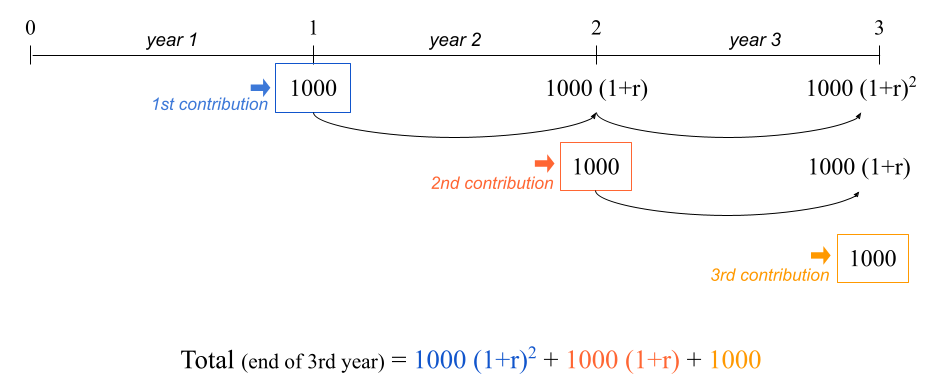
\includegraphics[width=0.95\linewidth]{images/conditionals/timeline-ord-annuity} 

}

\caption{Timeline of an ordinary annuity}\label{fig:unnamed-chunk-166}
\end{figure}

The balance in your savings account at the end of year 3 is given by:

\[
\underbrace{1000 (1 + 0.02)^2}_{\text{1st contribution}} + \underbrace{1000 (1 + 0.02)}_{\text{2nd contrib.}} + \underbrace{1000}_{\text{3rd contrib.}} = 3060.4
\]

which in R we can quickly calculate as:

\begin{Shaded}
\begin{Highlighting}[]
\DecValTok{1000} \SpecialCharTok{*}\NormalTok{ (}\FloatTok{1.02}\NormalTok{)}\SpecialCharTok{\^{}}\DecValTok{2} \SpecialCharTok{+} \DecValTok{1000} \SpecialCharTok{*}\NormalTok{ (}\FloatTok{1.02}\NormalTok{) }\SpecialCharTok{+} \DecValTok{1000}
\CommentTok{\#\textgreater{} [1] 3060.4}
\end{Highlighting}
\end{Shaded}

This example corresponds to what is formally called an \textbf{ordinary annuity}.
It is an annuity because the same amount of money is contributed every year.
It is ordinary because the contributions are made at the
\textbf{end of each period} (e.g.~end of each year).

The formula to calculate the \textbf{future value of an ordinary annuity} is given by:

\[
\text{FV} = \text{C} \times \left [ \frac{(1 + r)^t - 1}{r} \right]
\]

\begin{itemize}
\item
  \(\text{FV}\) = future value (how much you'll have)
\item
  \(\text{C}\) = constant periodic contribution
\item
  \(r\) = rate of return (e.g.~annual rate of return)
\item
  \(t\) = number of periods (e.g.~number of years)
\end{itemize}

Writing code in a less quick and dirty, we may type these commands:

\begin{Shaded}
\begin{Highlighting}[]
\CommentTok{\# at the end of year 3}
\NormalTok{contrib }\OtherTok{=} \DecValTok{1000}
\NormalTok{year }\OtherTok{=} \DecValTok{3}
\NormalTok{rate }\OtherTok{=} \FloatTok{0.02}

\CommentTok{\# FV of ordinary annuity}
\NormalTok{contrib }\SpecialCharTok{*}\NormalTok{ ((}\DecValTok{1} \SpecialCharTok{+}\NormalTok{ rate)}\SpecialCharTok{\^{}}\NormalTok{year }\SpecialCharTok{{-}} \DecValTok{1}\NormalTok{) }\SpecialCharTok{/}\NormalTok{ rate}
\CommentTok{\#\textgreater{} [1] 3060.4}
\end{Highlighting}
\end{Shaded}

\hypertarget{future-value-of-annuity-due}{%
\subsection{Future Value of Annuity Due}\label{future-value-of-annuity-due}}

It turns out that there is another type of annuity known as \textbf{annuity due}.
The difference between the ordinary annuity and the annuity due is that in the
latter the contributions are made at the \textbf{beginning of every year}. Here's an
example.

Picture the same hypothetical situation. Today is your first day of work
which corresponds to time 0, that is, the beginning of year 1 in your new job.
In this scenario, though, let's say you already have \$1000 at your disposal
at this point in time. You go to the bank and deposit this sum of money into a
savings account that pays an annual interest rate of 2\%.

During this first year you manage to save \$1000, and at the beginning of year 2
you make this contribution to your savings account. During your second year of
work, you manage again to save \$1000, which you add to your savings account at
the beginning of year 3. This is illustrated in the diagram below, with a
generic rate of return:

\begin{figure}

{\centering 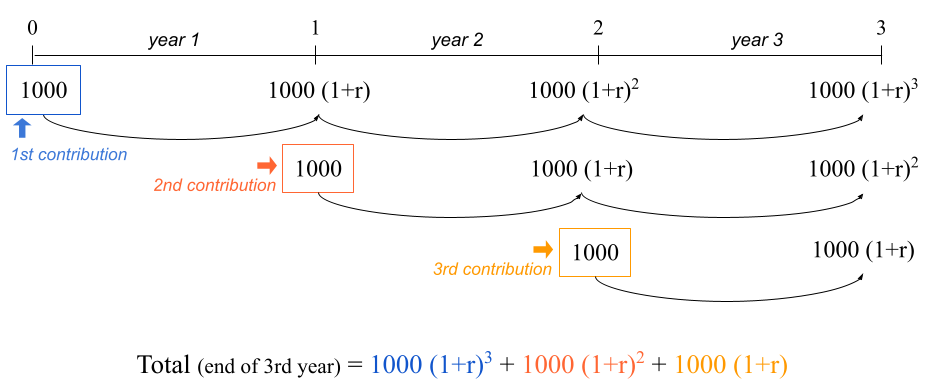
\includegraphics[width=0.95\linewidth]{images/conditionals/timeline-due-annuity} 

}

\caption{Timeline of an annuity due}\label{fig:unnamed-chunk-169}
\end{figure}

The balance in your savings account at the end of year 3 is given by:

\[
\underbrace{1000 (1 + 0.02)^3}_{\text{1st contribution}} + \underbrace{1000 (1 + 0.02)^2}_{\text{2nd contrib.}} + \underbrace{1000 (1 + 0.02)}_{\text{3rd contrib.}} = 3121.608
\]

which in R we can quickly calculate as:

\begin{Shaded}
\begin{Highlighting}[]
\DecValTok{1000} \SpecialCharTok{*}\NormalTok{ (}\FloatTok{1.02}\NormalTok{)}\SpecialCharTok{\^{}}\DecValTok{3} \SpecialCharTok{+} \DecValTok{1000} \SpecialCharTok{*}\NormalTok{ (}\DecValTok{1} \SpecialCharTok{+} \FloatTok{0.02}\NormalTok{)}\SpecialCharTok{\^{}}\DecValTok{2} \SpecialCharTok{+} \DecValTok{1000} \SpecialCharTok{*}\NormalTok{ (}\DecValTok{1} \SpecialCharTok{+} \FloatTok{0.02}\NormalTok{)}
\CommentTok{\#\textgreater{} [1] 3121.608}
\end{Highlighting}
\end{Shaded}

The formula to calculate the \textbf{future value of an annuity due} is given by:

\[
\text{FV} = \text{C} \times \left [ \frac{(1 + r)^t - 1}{r} \right] \times (1 + r)
\]

\begin{itemize}
\item
  \(\text{FV}\) = future value (how much you'll have)
\item
  \(\text{C}\) = constant periodic contribution
\item
  \(r\) = rate of return (e.g.~annual rate of return)
\item
  \(t\) = number of periods (e.g.~number of years)
\end{itemize}

In a less informal way, we can write the following lines of code:

\begin{Shaded}
\begin{Highlighting}[]
\CommentTok{\# at the end of year 3}
\NormalTok{contrib }\OtherTok{=} \DecValTok{1000}
\NormalTok{year }\OtherTok{=} \DecValTok{3}
\NormalTok{rate }\OtherTok{=} \FloatTok{0.02}

\CommentTok{\# FV of annuity due}
\NormalTok{contrib }\SpecialCharTok{*}\NormalTok{ (}\DecValTok{1} \SpecialCharTok{+}\NormalTok{ rate) }\SpecialCharTok{*}\NormalTok{ ((}\DecValTok{1} \SpecialCharTok{+}\NormalTok{ rate)}\SpecialCharTok{\^{}}\NormalTok{year }\SpecialCharTok{{-}} \DecValTok{1}\NormalTok{) }\SpecialCharTok{/}\NormalTok{ rate}
\CommentTok{\#\textgreater{} [1] 3121.608}
\end{Highlighting}
\end{Shaded}

As you know, we can also consider a vectorized option:

\begin{Shaded}
\begin{Highlighting}[]
\CommentTok{\# over a 3 year period}
\NormalTok{contrib }\OtherTok{=} \DecValTok{1000}
\NormalTok{years }\OtherTok{=} \DecValTok{1}\SpecialCharTok{:}\DecValTok{3}
\NormalTok{rate }\OtherTok{=} \FloatTok{0.02}

\CommentTok{\# FV of annuity due}
\NormalTok{contrib }\SpecialCharTok{*}\NormalTok{ (}\DecValTok{1} \SpecialCharTok{+}\NormalTok{ rate) }\SpecialCharTok{*}\NormalTok{ ((}\DecValTok{1} \SpecialCharTok{+}\NormalTok{ rate)}\SpecialCharTok{\^{}}\NormalTok{years }\SpecialCharTok{{-}} \DecValTok{1}\NormalTok{) }\SpecialCharTok{/}\NormalTok{ rate}
\CommentTok{\#\textgreater{} [1] 1020.000 2060.400 3121.608}
\end{Highlighting}
\end{Shaded}

\hypertarget{conditionals-1}{%
\section{Conditionals}\label{conditionals-1}}

There are two types of annuity:

\begin{itemize}
\item
  \textbf{ordinary} (contributions at the end of each period)
\item
  \textbf{due} (contributions at the beginning of each period)
\end{itemize}

What if you want to consider an input \textbf{\texttt{type}} that can take
two values: \texttt{type\ =\ "ordinary"} or \texttt{type\ =\ "due"}?

\begin{Shaded}
\begin{Highlighting}[]
\CommentTok{\# in 3 years}
\NormalTok{contrib }\OtherTok{=} \DecValTok{1000}
\NormalTok{years }\OtherTok{=} \DecValTok{1}\SpecialCharTok{:}\DecValTok{3}
\NormalTok{rate }\OtherTok{=} \FloatTok{0.02}
\end{Highlighting}
\end{Shaded}

Ordinary annuity:

\begin{Shaded}
\begin{Highlighting}[]
\CommentTok{\# if type == "ordinary"}
\NormalTok{contrib }\SpecialCharTok{*}\NormalTok{ ((}\DecValTok{1} \SpecialCharTok{+}\NormalTok{ rate)}\SpecialCharTok{\^{}}\NormalTok{years }\SpecialCharTok{{-}} \DecValTok{1}\NormalTok{) }\SpecialCharTok{/}\NormalTok{ rate}
\CommentTok{\#\textgreater{} [1] 1000.0 2020.0 3060.4}
\end{Highlighting}
\end{Shaded}

Annuity due:

\begin{Shaded}
\begin{Highlighting}[]
\CommentTok{\# if type == "due"}
\NormalTok{contrib }\SpecialCharTok{*}\NormalTok{ (}\DecValTok{1} \SpecialCharTok{+}\NormalTok{ rate) }\SpecialCharTok{*}\NormalTok{ ((}\DecValTok{1} \SpecialCharTok{+}\NormalTok{ rate)}\SpecialCharTok{\^{}}\NormalTok{years }\SpecialCharTok{{-}} \DecValTok{1}\NormalTok{) }\SpecialCharTok{/}\NormalTok{ rate}
\CommentTok{\#\textgreater{} [1] 1020.000 2060.400 3121.608}
\end{Highlighting}
\end{Shaded}

\hypertarget{if-else-conditions}{%
\subsection{If-else conditions}\label{if-else-conditions}}

Perhaps the best way for you to get introduced to \texttt{if-else} statements is to
see one for yourself, so here it is:

\begin{Shaded}
\begin{Highlighting}[]
\CommentTok{\# ordinary annuity}
\NormalTok{contrib }\OtherTok{=} \DecValTok{1000}
\NormalTok{years }\OtherTok{=} \DecValTok{1}\SpecialCharTok{:}\DecValTok{3}
\NormalTok{rate }\OtherTok{=} \FloatTok{0.02}
\NormalTok{type }\OtherTok{=} \StringTok{"ordinary"}

\CommentTok{\# if{-}else statement}
\ControlFlowTok{if}\NormalTok{ (type }\SpecialCharTok{==} \StringTok{"ordinary"}\NormalTok{) \{}
\NormalTok{  fv }\OtherTok{=}\NormalTok{ contrib }\SpecialCharTok{*}\NormalTok{ ((}\DecValTok{1} \SpecialCharTok{+}\NormalTok{ rate)}\SpecialCharTok{\^{}}\NormalTok{years }\SpecialCharTok{{-}} \DecValTok{1}\NormalTok{) }\SpecialCharTok{/}\NormalTok{ rate}
\NormalTok{\} }\ControlFlowTok{else}\NormalTok{ \{}
\NormalTok{  fv }\OtherTok{=}\NormalTok{ contrib }\SpecialCharTok{*}\NormalTok{ (}\DecValTok{1} \SpecialCharTok{+}\NormalTok{ rate) }\SpecialCharTok{*}\NormalTok{ ((}\DecValTok{1} \SpecialCharTok{+}\NormalTok{ rate)}\SpecialCharTok{\^{}}\NormalTok{years }\SpecialCharTok{{-}} \DecValTok{1}\NormalTok{) }\SpecialCharTok{/}\NormalTok{ rate}
\NormalTok{\}}

\NormalTok{fv}
\CommentTok{\#\textgreater{} [1] 1000.0 2020.0 3060.4}
\end{Highlighting}
\end{Shaded}

I hope that just by looking at the conditional statement you get the gist of
what is going on. If the type of annuity is the ordinary one
(\texttt{type\ ==\ "ordinary"}) then we apply the formula of the FV of ordinary annuity.
Otherwise (\texttt{else}) we apply the formula of the FV of annuity due.

The same piece of code can be implemented with the other type of annuity

\begin{Shaded}
\begin{Highlighting}[]
\CommentTok{\# annuity due}
\NormalTok{contrib }\OtherTok{=} \DecValTok{1000}
\NormalTok{years }\OtherTok{=} \DecValTok{1}\SpecialCharTok{:}\DecValTok{3}
\NormalTok{rate }\OtherTok{=} \FloatTok{0.02}
\NormalTok{type }\OtherTok{=} \StringTok{"due"}
  
\ControlFlowTok{if}\NormalTok{ (type }\SpecialCharTok{==} \StringTok{"ordinary"}\NormalTok{) \{}
\NormalTok{  fv }\OtherTok{=}\NormalTok{ contrib }\SpecialCharTok{*}\NormalTok{ ((}\DecValTok{1} \SpecialCharTok{+}\NormalTok{ rate)}\SpecialCharTok{\^{}}\NormalTok{years }\SpecialCharTok{{-}} \DecValTok{1}\NormalTok{) }\SpecialCharTok{/}\NormalTok{ rate}
\NormalTok{\} }\ControlFlowTok{else}\NormalTok{ \{}
\NormalTok{  fv }\OtherTok{=}\NormalTok{ contrib }\SpecialCharTok{*}\NormalTok{ (}\DecValTok{1} \SpecialCharTok{+}\NormalTok{ rate) }\SpecialCharTok{*}\NormalTok{ ((}\DecValTok{1} \SpecialCharTok{+}\NormalTok{ rate)}\SpecialCharTok{\^{}}\NormalTok{years }\SpecialCharTok{{-}} \DecValTok{1}\NormalTok{) }\SpecialCharTok{/}\NormalTok{ rate}
\NormalTok{\}}

\NormalTok{fv}
\CommentTok{\#\textgreater{} [1] 1020.000 2060.400 3121.608}
\end{Highlighting}
\end{Shaded}

\hypertarget{anatomy-of-if-else-statements}{%
\subsection{Anatomy of if-else statements}\label{anatomy-of-if-else-statements}}

The \textbf{if-then-else} statement makes it possible to choose between two
(possibly compound) expressions depending on the value of a (logical) condition.

In R (as in many other languages) the if-then-else statement has the following
structure:

\begin{Shaded}
\begin{Highlighting}[]
\ControlFlowTok{if}\NormalTok{ (condition) \{}
  \CommentTok{\# do something}
\NormalTok{\} }\ControlFlowTok{else}\NormalTok{ \{}
  \CommentTok{\# do something else}
\NormalTok{\}}
\end{Highlighting}
\end{Shaded}

In our working example with the two types of annuities, the condition that
we are evaluating depends on the value of \texttt{type}:

\begin{Shaded}
\begin{Highlighting}[]
\ControlFlowTok{if}\NormalTok{ (type }\SpecialCharTok{==} \StringTok{"ordinary"}\NormalTok{) \{}
  \CommentTok{\# compute ordinary annuity}
\NormalTok{\} }\ControlFlowTok{else}\NormalTok{ \{}
  \CommentTok{\# compute annuity due}
\NormalTok{\}}
\end{Highlighting}
\end{Shaded}

If \texttt{type\ ==\ "ordinary"},
then we should compute the future value of annuity using its ordinary version.
Otherwise, we should compute the future value using the annuity due formula.

Let's dissect the conditional statement

\begin{center}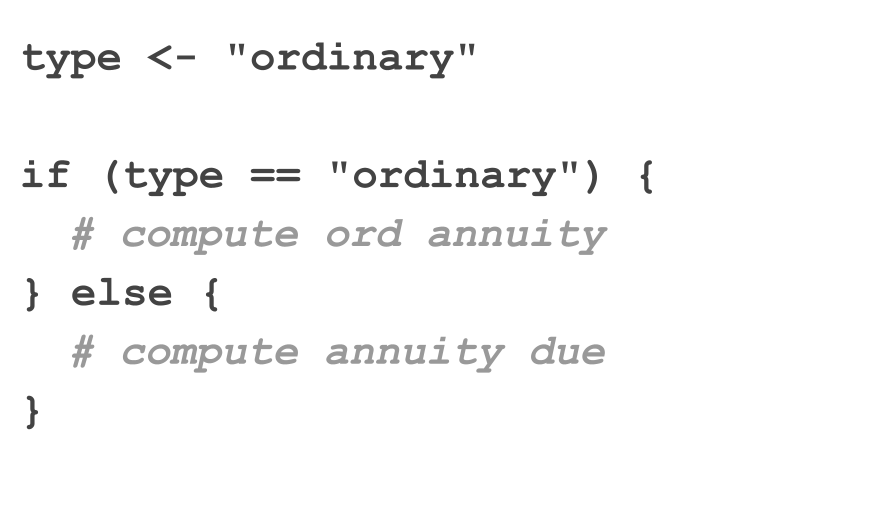
\includegraphics[width=0.5\linewidth]{images/conditionals/if-else-anatomy-1} \end{center}

An \texttt{if-else} statement always begins with the \texttt{if} clause. You basically refer
to it as a function, that is, employing parenthesis \texttt{if(\ )}. The thing that
goes inside parenthesis corresponds to the logical condition to be evaluated.
Then we have the R expression, defined with the first pair of braces \texttt{\{\ \}} that
contains the code to be executed when the logical condition is true. Next,
right after the closing brace of the expression associated to the if-clause, we
have the \texttt{else} clause. This second clause involves another R expression, the
one defined with a second pair of braces. This expression contains the code to
be executed when the logical condition is false.

For readability purposes, and to match the syntax used in many other programming
languages, when declaring the \texttt{if} clause I prefer to leave a blank space before
the opening parenthesis: \texttt{if\ (condition)}.

Using the annuity example, let's recap the main parts of a typical if-else
statement. In general, this kind of statement consists of the \texttt{if} clause
and the \texttt{else} clause. Only the \texttt{if} clause uses parenthesis.

\begin{center}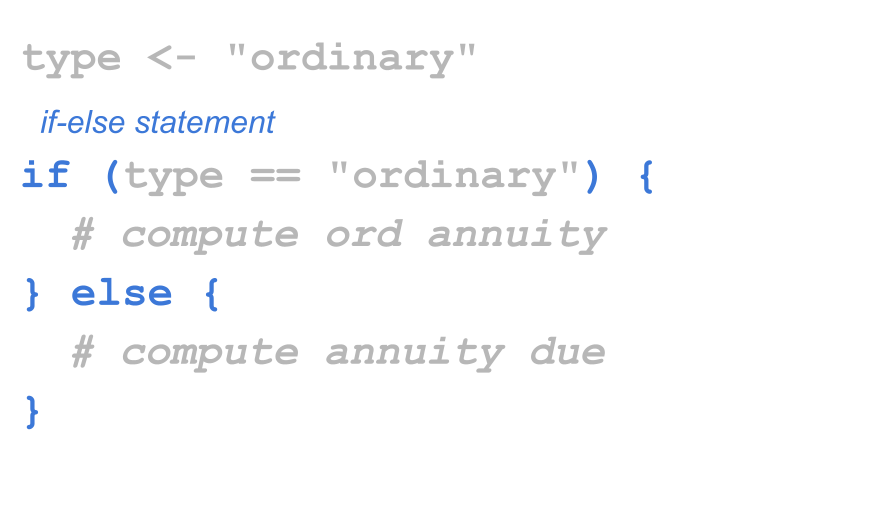
\includegraphics[width=0.5\linewidth]{images/conditionals/if-else-anatomy-2} \end{center}

Inside the \texttt{if()} function, you specify a \textbf{condition} to be
evaluated. This condition can be almost any piece of code that R will evaluate
into a \textbf{logical} value. The important thing about this condition is that it
must correspond to a single logical value, either a single \texttt{TRUE} or a single
\texttt{FALSE}.

The \emph{condition} is an expression that when evaluated returns
a \textbf{logical} value of length one. In other words, whatever you pass as the
input of the \texttt{if} clause, it has to be something that becomes \texttt{TRUE} or \texttt{FALSE}

\begin{center}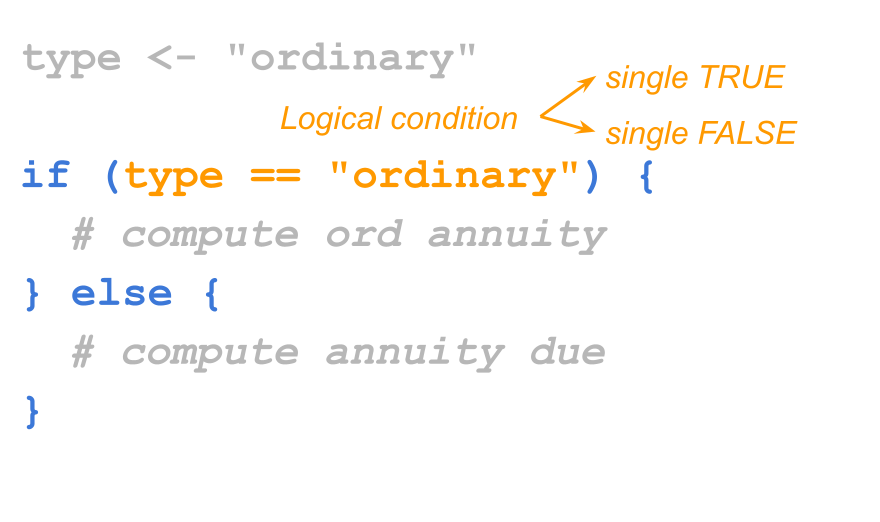
\includegraphics[width=0.5\linewidth]{images/conditionals/if-else-anatomy-3} \end{center}

In general, an R expression---using braces \texttt{\{\ \}}---is used for each clause:
the first one with the code that tells R what to do when the evaluated
condition is true; the second one for what to do when the condition is false.

\begin{center}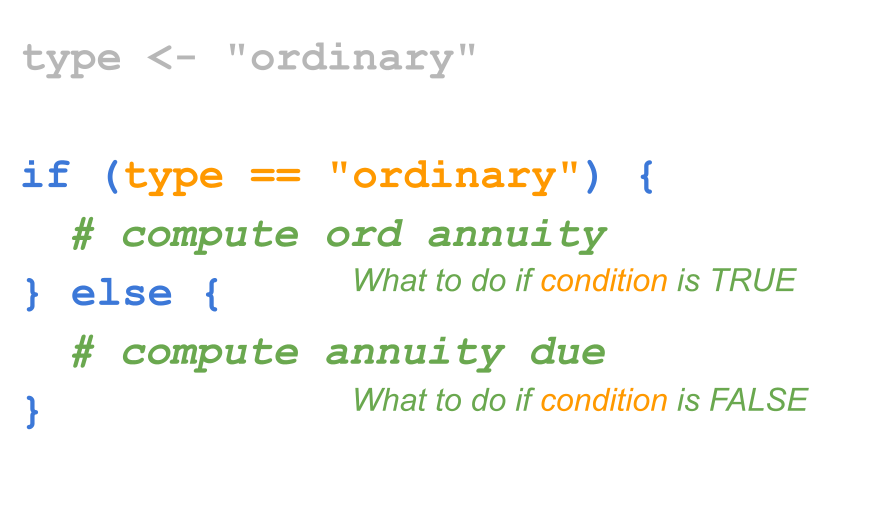
\includegraphics[width=0.5\linewidth]{images/conditionals/if-else-anatomy-6} \end{center}

\hypertarget{minimalist-if-then-else}{%
\subsection{Minimalist If-then-else}\label{minimalist-if-then-else}}

\texttt{if-else} statements can be written in different forms, depending on the types
of expressions that are evaluated. If the expressions of both the \texttt{if} clause
and the \texttt{else} clause are \textbf{simple} expressions, the syntax of the \texttt{if-else}
code can be simplified into one line of code:

\begin{Shaded}
\begin{Highlighting}[]
\ControlFlowTok{if}\NormalTok{ (condition) expression\_1 }\ControlFlowTok{else}\NormalTok{ expression\_2}
\end{Highlighting}
\end{Shaded}

Consider the following example that uses a conditional statement to decide
between calculating the square root of the input \emph{if} the input value is
positive, or computing the negative square root of the negative input \emph{if} the
input value is negative:

\begin{Shaded}
\begin{Highlighting}[]
\NormalTok{x }\OtherTok{\textless{}{-}} \DecValTok{10}

\ControlFlowTok{if}\NormalTok{ (x }\SpecialCharTok{\textgreater{}} \DecValTok{0}\NormalTok{) \{}
\NormalTok{  y }\OtherTok{\textless{}{-}} \FunctionTok{sqrt}\NormalTok{(x) }
\NormalTok{\} }\ControlFlowTok{else}\NormalTok{ \{}
\NormalTok{  y }\OtherTok{\textless{}{-}} \SpecialCharTok{{-}}\FunctionTok{sqrt}\NormalTok{(}\SpecialCharTok{{-}}\NormalTok{x)}
\NormalTok{\}}
\NormalTok{y}
\CommentTok{\#\textgreater{} [1] 3.162278}
\end{Highlighting}
\end{Shaded}

Because the code in both clauses consists of simple expressions, the use of
braces is not mandatory. In fact, you can write the conditional statement in
a single line of code, as follows:

\begin{Shaded}
\begin{Highlighting}[]
\NormalTok{x }\OtherTok{\textless{}{-}} \DecValTok{10}

\CommentTok{\# with simple expressions, braces are optional}
\ControlFlowTok{if}\NormalTok{ (x }\SpecialCharTok{\textgreater{}} \DecValTok{0}\NormalTok{) y }\OtherTok{\textless{}{-}} \FunctionTok{sqrt}\NormalTok{(x) }\ControlFlowTok{else}\NormalTok{ y }\OtherTok{\textless{}{-}} \SpecialCharTok{{-}}\FunctionTok{sqrt}\NormalTok{(}\SpecialCharTok{{-}}\NormalTok{x)}

\NormalTok{y}
\end{Highlighting}
\end{Shaded}

Interestingly, the previous statement can be written more succinctly in R as:

\begin{Shaded}
\begin{Highlighting}[]
\NormalTok{x }\OtherTok{\textless{}{-}} \DecValTok{10}

\CommentTok{\# you can assign the output of an if{-}else statement}
\CommentTok{\# to an object}
\NormalTok{y }\OtherTok{\textless{}{-}} \ControlFlowTok{if}\NormalTok{ (x }\SpecialCharTok{\textgreater{}} \DecValTok{0}\NormalTok{) }\FunctionTok{sqrt}\NormalTok{(x) }\ControlFlowTok{else} \SpecialCharTok{{-}}\FunctionTok{sqrt}\NormalTok{(}\SpecialCharTok{{-}}\NormalTok{x)}

\NormalTok{y}
\end{Highlighting}
\end{Shaded}

Again, even though the previous commands are perfectly okay, I prefer to
use braces when working with conditional structures. This is a good practice
that improves readability:

\begin{Shaded}
\begin{Highlighting}[]
\CommentTok{\# embrace braces: use them as much as possible!}
\NormalTok{x }\OtherTok{\textless{}{-}} \DecValTok{10}

\ControlFlowTok{if}\NormalTok{ (x }\SpecialCharTok{\textgreater{}} \DecValTok{0}\NormalTok{) \{}
\NormalTok{  y }\OtherTok{\textless{}{-}} \FunctionTok{sqrt}\NormalTok{(x) }
\NormalTok{\} }\ControlFlowTok{else}\NormalTok{ \{}
\NormalTok{  y }\OtherTok{\textless{}{-}} \SpecialCharTok{{-}}\FunctionTok{sqrt}\NormalTok{(}\SpecialCharTok{{-}}\NormalTok{x)}
\NormalTok{\}}
\end{Highlighting}
\end{Shaded}

\hypertarget{simple-ifs}{%
\subsection{Simple If's}\label{simple-ifs}}

There is a simplified form of if-else statement which is available when
there is no expression in the \texttt{else} clause. In its simplest version this
statement has the general form:

\begin{Shaded}
\begin{Highlighting}[]
\ControlFlowTok{if}\NormalTok{ (condition) expression}
\end{Highlighting}
\end{Shaded}

and it is equivalent to:

\begin{Shaded}
\begin{Highlighting}[]
\ControlFlowTok{if}\NormalTok{ (condition) expression }\ControlFlowTok{else} \ConstantTok{NULL}
\end{Highlighting}
\end{Shaded}

Here's an example in which we have two numbers, \texttt{x} and \texttt{y}, and we are
interested in knowing if \texttt{x} is greater than \texttt{y}. If yes, we print the message
\texttt{"x\ is\ greater\ than\ y"}. If not, then we don't really care, and we do nothing.

\begin{Shaded}
\begin{Highlighting}[]
\NormalTok{x }\OtherTok{\textless{}{-}} \DecValTok{4}
\NormalTok{y }\OtherTok{\textless{}{-}} \DecValTok{2}

\ControlFlowTok{if}\NormalTok{ (x }\SpecialCharTok{\textgreater{}}\NormalTok{ y) \{}
  \FunctionTok{print}\NormalTok{(}\StringTok{"x is greater than y"}\NormalTok{)}
\NormalTok{\}}
\CommentTok{\#\textgreater{} [1] "x is greater than y"}
\end{Highlighting}
\end{Shaded}

\hypertarget{multiple-ifs}{%
\section{Multiple If's}\label{multiple-ifs}}

A common situation involves working with multiple conditions at the same time.
You can chain multiple if-else statements like so:

\begin{Shaded}
\begin{Highlighting}[]
\NormalTok{y }\OtherTok{\textless{}{-}} \DecValTok{1} \CommentTok{\# Change this value!}

\ControlFlowTok{if}\NormalTok{ (y }\SpecialCharTok{\textgreater{}} \DecValTok{0}\NormalTok{) \{}
  \FunctionTok{print}\NormalTok{(}\StringTok{"positive"}\NormalTok{)}
\NormalTok{\} }\ControlFlowTok{else} \ControlFlowTok{if}\NormalTok{ (y }\SpecialCharTok{\textless{}} \DecValTok{0}\NormalTok{) \{}
  \FunctionTok{print}\NormalTok{(}\StringTok{"negative"}\NormalTok{)}
\NormalTok{\} }\ControlFlowTok{else}\NormalTok{ \{}
  \FunctionTok{print}\NormalTok{(}\StringTok{"zero?"}\NormalTok{)}
\NormalTok{\}}
\CommentTok{\#\textgreater{} [1] "positive"}
\end{Highlighting}
\end{Shaded}

Working with multiple chained if's becomes cumbersome. Consider the following
example that uses several if's to convert a day of the week into a number:

\begin{Shaded}
\begin{Highlighting}[]
\CommentTok{\# Convert the day of the week into a number.}
\NormalTok{day }\OtherTok{\textless{}{-}} \StringTok{"Tuesday"} \CommentTok{\# Change this value!}

\ControlFlowTok{if}\NormalTok{ (day }\SpecialCharTok{==} \StringTok{\textquotesingle{}Sunday\textquotesingle{}}\NormalTok{) \{}
\NormalTok{  num\_day }\OtherTok{\textless{}{-}} \DecValTok{1}
\NormalTok{\} }\ControlFlowTok{else}\NormalTok{ \{}
  \ControlFlowTok{if}\NormalTok{ (day }\SpecialCharTok{==} \StringTok{"Monday"}\NormalTok{) \{}
\NormalTok{    num\_day }\OtherTok{\textless{}{-}} \DecValTok{2}
\NormalTok{  \} }\ControlFlowTok{else}\NormalTok{ \{}
    \ControlFlowTok{if}\NormalTok{ (day }\SpecialCharTok{==} \StringTok{"Tuesday"}\NormalTok{) \{}
\NormalTok{      num\_day }\OtherTok{\textless{}{-}} \DecValTok{3}
\NormalTok{    \} }\ControlFlowTok{else}\NormalTok{ \{}
      \ControlFlowTok{if}\NormalTok{ (day }\SpecialCharTok{==} \StringTok{"Wednesday"}\NormalTok{) \{}
\NormalTok{        num\_day }\OtherTok{\textless{}{-}} \DecValTok{4}
\NormalTok{      \} }\ControlFlowTok{else}\NormalTok{ \{}
        \ControlFlowTok{if}\NormalTok{ (day }\SpecialCharTok{==} \StringTok{"Thursday"}\NormalTok{) \{}
\NormalTok{          num\_day }\OtherTok{\textless{}{-}} \DecValTok{5}
\NormalTok{        \} }\ControlFlowTok{else}\NormalTok{ \{}
          \ControlFlowTok{if}\NormalTok{ (day }\SpecialCharTok{==} \StringTok{"Friday"}\NormalTok{) \{}
\NormalTok{            num\_day }\OtherTok{\textless{}{-}} \DecValTok{6}
\NormalTok{          \} }\ControlFlowTok{else}\NormalTok{ \{}
            \ControlFlowTok{if}\NormalTok{ (day }\SpecialCharTok{==} \StringTok{"Saturday"}\NormalTok{) \{}
\NormalTok{              num\_day }\OtherTok{\textless{}{-}} \DecValTok{7}
\NormalTok{            \}}
\NormalTok{          \}}
\NormalTok{        \}}
\NormalTok{      \}}
\NormalTok{    \}}
\NormalTok{  \}}
\NormalTok{\}}

\NormalTok{num\_day}
\CommentTok{\#\textgreater{} [1] 3}
\end{Highlighting}
\end{Shaded}

Working with several nested if's like in the example above can be a nightmare.

In R, you can get rid of many of the braces like this:

\begin{Shaded}
\begin{Highlighting}[]
\CommentTok{\# Convert the day of the week into a number.}
\NormalTok{day }\OtherTok{\textless{}{-}} \StringTok{"Tuesday"} \CommentTok{\# Change this value!}

\ControlFlowTok{if}\NormalTok{ (day }\SpecialCharTok{==} \StringTok{\textquotesingle{}Sunday\textquotesingle{}}\NormalTok{) \{}
\NormalTok{  num\_day }\OtherTok{\textless{}{-}} \DecValTok{1}
\NormalTok{\} }\ControlFlowTok{else} \ControlFlowTok{if}\NormalTok{ (day }\SpecialCharTok{==} \StringTok{"Monday"}\NormalTok{) \{}
\NormalTok{  num\_day }\OtherTok{\textless{}{-}} \DecValTok{2}
\NormalTok{\} }\ControlFlowTok{else} \ControlFlowTok{if}\NormalTok{ (day }\SpecialCharTok{==} \StringTok{"Tuesday"}\NormalTok{) \{}
\NormalTok{  num\_day }\OtherTok{\textless{}{-}} \DecValTok{3}
\NormalTok{\} }\ControlFlowTok{else} \ControlFlowTok{if}\NormalTok{ (day }\SpecialCharTok{==} \StringTok{"Wednesday"}\NormalTok{) \{}
\NormalTok{  num\_day }\OtherTok{\textless{}{-}} \DecValTok{4}
\NormalTok{\} }\ControlFlowTok{else} \ControlFlowTok{if}\NormalTok{ (day }\SpecialCharTok{==} \StringTok{"Thursday"}\NormalTok{) \{}
\NormalTok{  num\_day }\OtherTok{\textless{}{-}} \DecValTok{5}
\NormalTok{\} }\ControlFlowTok{else} \ControlFlowTok{if}\NormalTok{ (day }\SpecialCharTok{==} \StringTok{"Friday"}\NormalTok{) \{}
\NormalTok{  num\_day }\OtherTok{\textless{}{-}} \DecValTok{6}
\NormalTok{\} }\ControlFlowTok{else} \ControlFlowTok{if}\NormalTok{ (day }\SpecialCharTok{==} \StringTok{"Saturday"}\NormalTok{) \{}
\NormalTok{  num\_day }\OtherTok{\textless{}{-}} \DecValTok{7}
\NormalTok{\}}

\NormalTok{num\_day}
\CommentTok{\#\textgreater{} [1] 3}
\end{Highlighting}
\end{Shaded}

\hypertarget{switch-statements}{%
\subsection{Switch statements}\label{switch-statements}}

But still we have too many if's, and there's a lot of repetition in the code.
If you find yourself using many if-else statements with identical structure for
slightly different cases, you may want to consider a \textbf{switch} statement
instead:

\begin{Shaded}
\begin{Highlighting}[]
\CommentTok{\# Convert the day of the week into a number.}
\NormalTok{day }\OtherTok{\textless{}{-}} \StringTok{"Tuesday"} \CommentTok{\# Change this value!}

\ControlFlowTok{switch}\NormalTok{(day, }\CommentTok{\# The expression to be evaluated.}
  \AttributeTok{Sunday =} \DecValTok{1}\NormalTok{,}
  \AttributeTok{Monday =} \DecValTok{2}\NormalTok{,}
  \AttributeTok{Tuesday =} \DecValTok{3}\NormalTok{,}
  \AttributeTok{Wednesday =} \DecValTok{4}\NormalTok{,}
  \AttributeTok{Thursday =} \DecValTok{5}\NormalTok{,}
  \AttributeTok{Friday =} \DecValTok{6}\NormalTok{,}
  \AttributeTok{Saturday =} \DecValTok{7}\NormalTok{,}
  \ConstantTok{NA}\NormalTok{) }\CommentTok{\# an (optional) default value if there are no matches}
\CommentTok{\#\textgreater{} [1] 3}
\end{Highlighting}
\end{Shaded}

Switch statements can also accept integer arguments, which will act as indices
to choose a corresponding element:

\begin{Shaded}
\begin{Highlighting}[]
\CommentTok{\# Convert a number into a day of the week.}
\NormalTok{day\_num }\OtherTok{\textless{}{-}} \DecValTok{3} \CommentTok{\# Change this value!}

\ControlFlowTok{switch}\NormalTok{(day\_num,}
  \StringTok{"Sunday"}\NormalTok{,}
  \StringTok{"Monday"}\NormalTok{,}
  \StringTok{"Tuesday"}\NormalTok{,}
  \StringTok{"Wednesday"}\NormalTok{,}
  \StringTok{"Thursday"}\NormalTok{,}
  \StringTok{"Friday"}\NormalTok{,}
  \StringTok{"Saturday"}\NormalTok{)}
\CommentTok{\#\textgreater{} [1] "Tuesday"}
\end{Highlighting}
\end{Shaded}

\hypertarget{derivation-of-fvoa}{%
\section{Derivation of FVOA}\label{derivation-of-fvoa}}

In case you are curious, here's the derivation of the formula for the
Future Value of an Ordinary Annuity.

For the sake of illustration, we'll consider a time period of three years,
but the formula can be easily generalized to any number of years.

\begin{figure}

{\centering 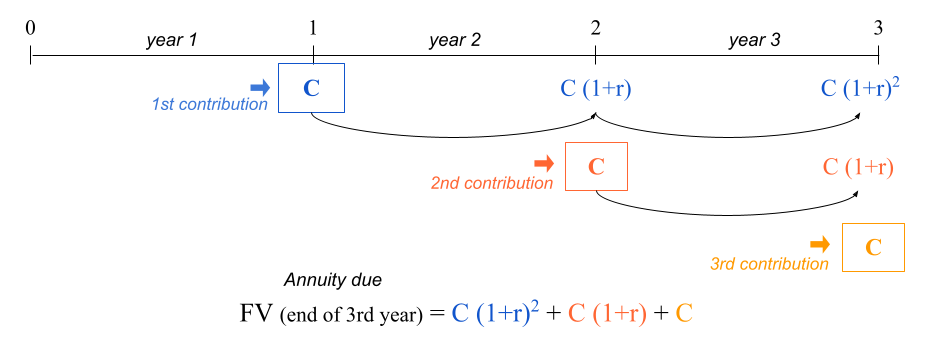
\includegraphics[width=0.95\linewidth]{images/conditionals/timeline-ord-annuity-2} 

}

\caption{Timeline of an ordinary annuity}\label{fig:unnamed-chunk-189}
\end{figure}

The starting point is the following equation:

\[
\text{FV} = \text{C} + \text{C} (1 + r) + \text{C} (1 + r)^2
\]

Multiplying both sides by \((1+r)\) we get:

\begin{align*}
(1+r) \text{FV} &= (1+r) \left[ \text{C} + \text{C} (1 + r) + \text{C} (1 + r)^2 \right] \\
(1+r) \text{FV} &= (1+r) \text{C} + \text{C} (1 + r)^2 + \text{C} (1 + r)^3
\end{align*}

Notice that:

\[
(1+r) \text{FV} = \underbrace{\text{C} (1 + r) + \text{C} (1 + r)^2}_{\text{FV} - \text{C}}  + \text{C} (1 + r)^3
\]

Doing more algebra we get the following:

\begin{align*}
(1+r) \text{FV} &= \underbrace{\text{C} (1 + r) + \text{C} (1 + r)^2}_{\text{FV} - \text{C}}  + \text{C} (1 + r)^3 \\
(1+r) \text{FV} &= \text{FV} - \text{C} + \text{C} (1 + r)^3 \\
\text{FV} - (1+r) \text{FV} &= \text{C} - \text{C}(1+r)^3 \\
\text{FV} \left[ 1 - (1+r)  \right] &= \text{C} \left[ 1 - (1+r)^3 \right] \\
\text{FV} &= \text{C} \frac{ \left[ 1 - (1+r)^3 \right]}{ \left[ 1 - (1+r) \right]} \\
\text{FV} &= \text{C} \frac{ \left[ (1+r)^3 -1 \right]}{ \left[ (1+r) -1 \right]} \\
\text{FV} &= \text{C} \left[ \frac{(1+r)^3 -1}{r} \right]
\end{align*}

Therefore:

\[
\text{FV} = \text{C} + \text{C} (1 + r) + \text{C} (1 + r)^2 = \text{C} \left[ \frac{(1+r)^3 -1}{r} \right]
\]

  \bibliography{book.bib}

\end{document}
